%%%%%%%%%%%%%%%%%%%%%%%%%%%%%%%%%%%%%%%%%%%%%%%%%%%%%%%%%%%%%%%%%%%%%%
% Lớp 11 | Quan hệ vuông góc trong không gian | Hai đường thẳng vuông góc
% Dạng 1H8?1-3: Tìm góc giữa hai đường thẳng
% Số câu: 152  (sinh tự động bởi tach_cau.py; từ nay thầy sửa trực tiếp file này)
%%%%%%%%%%%%%%%%%%%%%%%%%%%%%%%%%%%%%%%%%%%%%%%%%%%%%%%%%%%%%%%%%%%%%%

%%%%%%%%%%%%%%%% TRẮC NGHIỆM 4 PHƯƠNG ÁN %%%%%%%%%%%%%%%%

% nguồn: Ok_TracNghiemLop11_Lan1
\begin{ex}%[1H8N1-3]%[ma:afe4aa91]
	 \immini
	 {
	Cho hình chóp $S.ABC$, cạnh bên $SB$ vuông  góc với đáy $(ABC)$. Gọi $\alpha$ là số đo của góc tạo bởi đường thẳng $SB$ và $AC$. Mệnh đề nào sau đây đúng?
	\choice 
		{$\alpha >90^\circ$} 
		{$\alpha  <90^\circ$}
		 {$\alpha >180^\circ$}
		{\True $\alpha  =90^\circ$}
		 }
		 {
		\begin{tikzpicture}[font=\footnotesize,line join=round,line cap=round,>=stealth,scale=.7]
				\foreach \x/\y/\pos in {0/0/B,4/0/C,1.5/-2/A}  \path ($(\x,\y)$) coordinate (\pos);
				 \path
					 ($(B)+(0,3)$) coordinate (S);
				\draw[dashed]  (B)--(C);
				\draw  (S)--(B)--(A)--(C)--cycle (S)--(A);
				\foreach \x/\pos in {A/-90,S/90,B/180,C/0} \fill (\x) circle (1pt)  node[{shift=(\pos:0.25)}]{$\x$};
			\end{tikzpicture}
		} 
	 \loigiai{
		Do $SB\perp (ABC)$ nên $SB\perp  AC$ hay góc $\alpha=90^\circ$.
	 }
\end{ex}

% nguồn: Ok_TracNghiemLop11_Lan1
\begin{ex}%[1H8N1-3]%[ma:1d601189]
	Cho hình lập phương $ABCD \cdot A^{\prime} B^{\prime} C^{\prime}  D^{\prime}$. Góc giữa hai đường thẳng $AA^{\prime}$ và $CD$ bằng
	\choice 
		 {$30^{\circ}$}
		{\True $90^{\circ}$} 
		 {$45^{\circ}$}
		{$60^{\circ}$} 
	 \loigiai{
	\immini{ 
		 Ta có $CD\parallel AB$ suy ra $(AA',CD)=(AA',AB)=90^\circ$.
		} 
		{\begin{tikzpicture}
		\def\a{2.5} 
		\path (0:0) coordinate  (A)
			++(0:\a) coordinate  (D)
			 ++(-130:\a/2) coordinate (C)
			 ($(A)+(C)-(D)$) coordinate (B)
			 ($(A)+(90:\a)$) coordinate (A')
			($(B)+(90:\a)$)  coordinate (B')
			($(C)+(90:\a)$) coordinate (C') 
			 ($(D)+(90:\a)$) coordinate (D');
		\draw[dashed] (B)--(A)--(D) 
			 (A)--(A');
		\draw  (C)--(C')
			(D)--(D') 
			 (B)--(B')
			 (B)--(C)--(D)
			 (A')--(B')--(C')--(D')--cycle;
		 \foreach \x/\g in {A/180,B/180,C/0,D/0,A'/180,B'/180,C'/0,D'/0}
		\fill[black] (\x)  circle (1pt)
			($(\g:4mm)+(\x)$) node  {$\x$};
	\end{tikzpicture}
		} 
	} 
\end{ex}

% nguồn: Ok_TracNghiemLop11_Lan1
\begin{ex}%[1H8N1-3]%[ma:03c5e9e7]
	[Dự án đề kiểm tra giữa học kỳ 2 khối 11 NH23-24-Đợt 11- Bùi Thanh  Cương]
	 \immini
	{ 
	Cho hình lập phương $ ABCD.A'B'C'D'$. Góc giữa hai đường thằng $A'B$ và  $CD$ bằng
	 \choice
		 {$60^{\circ}$}
		 {$30^{\circ}$}
		{\True $45^{\circ}$} 
		 {$90^{\circ}$}
		 }
		{ 
		\begin{tikzpicture}[line join=round,line cap=round,scale=0.7]
				\def\h{3} 
				 \path
					(0,0) coordinate  (A)
					(3.5,0) coordinate  (D)
					 (-1.5,-1.5) coordinate (B);
				\path  ($(B)+(D)-(A)$) coordinate (C);
				\foreach  \diem/\anh in {A/A',B/B',C/C',D/D'} \coordinate (\anh) at ($(0,\h)+(\diem)-(A)$);
				\path (intersection  of A'--C and A--C') coordinate (O);
				\draw (A')--(B')--(C')--(D')--cycle; 
				 \draw (B)--(C)--(D);
				\draw  (B)--(B')
					 (C)--(C')
					(D)--(D'); 
				\draw[dashed]  (A)--(B)
					(A)--(D) 
					(A)--(A') 
					(A')--(B); 
				\foreach  \i/\j in {A/140,B/-160,C/-20,D/-20,A'/140,B'/-160,C'/-20,D'/40}\fill (\i) circle (1pt)
					($(\i) +  (\j:5mm)$) node{$\i$};
			\end{tikzpicture}
		 }
	\loigiai{ 
		Ta  có $AB\parallel CD$ nên góc $\left(A'B; CD\right)=\left(A'B; AB\right)=\widehat{A'BA}=45^{\circ}$.\\
		Vậy giữa hai đường thằng $A'B$ và  $CD$ bằng $45^{\circ}$.
	 }
\end{ex}

% nguồn: Ok_TracNghiemLop11_Lan1
\begin{ex}%[1H8N1-3]%[ma:b1c4ab6c]
	Cho  hình lập phương $ABCD.A_1B_1C_1D_1$. Góc giữa $AC$ và $DA_1$ là
	\choice 
		 {$90^{\circ}$}
		{\True  $60^{\circ}$}
		 {$45^{\circ}$}
		{$120^{\circ}$} 
	\loigiai{ 
	\immini{ 
		Vì $A_1C_1 \parallel AC$ nên góc giữa $AC$ và $DA_1$ bằng  góc giữa $A_1C_1$ và $DA_1$. \\
		Do  tam giác $DA_1C_1$ đều nên $\widehat{DA_1C_1}=60^{\circ}$.\\
		Vậy góc giữa $AC$ và $DA_1$ bằng  $60^{\circ}$.
		}{ 
		\begin{tikzpicture}[scale=0.6,font=\footnotesize,line join=round,line cap=round,>=stealth]
				\coordinate  (a) at (2,2);
				\coordinate (b) at  (0,0);
				\coordinate (c) at (5,0); 
				\coordinate (d) at  (7,2);
				\coordinate (a1) at  ($(a)+(0,5)$);
				\coordinate  (b1) at ($(b)+(0,5)$);
				\coordinate  (c1) at ($(c)+(0,5)$);
				\coordinate (d1) at  ($(d)+(0,5)$);
				\draw[dashed] (b) -- (a) --  (d)
					 (a) -- (a1);
				\draw (b) -- (c) -- (d) -- (d1) -- (c1) -- (b1) -- (a1) -- (d1) 
					(b) -- (b1) 
					 (c) -- (c1);
				\draw (a)  node[below]{$A$};
				\draw (b)  node[below]{$B$};
				\draw (c) node[below]{$C$}; 
				\draw (d)  node[right]{$D$};
				 \draw (a1) node[above]{$A_1$};
				\draw (b1) node[below left]{$B_1$}; 
				\draw (c1)  node[below right]{$C_1$};
				\draw (d1) node[right]{$D_1$}; 
				\draw[dashed]  (a)-- (c)
					(d) -- (a1); 
				\draw (a1) --  (c1);
			\end{tikzpicture}
		} 
	} 
\end{ex}

% nguồn: Ok_TracNghiemLop11_Lan1
\begin{ex}%[1H8N1-3]%[ma:3a4cddfc]
	Cho hình lập phương $ABCD.A'B'C'D'$. Góc giữa hai đường thẳng  $BA'$ và $CD$ bằng:
	\choice 
		{\True $45^\circ $} 
		 {$60^\circ $}
		{$30^\circ $} 
		{$90^\circ $} 
	\loigiai{ 
		\begin{tikzpicture}[scale=1,font=\footnotesize,line join=round,line cap=round,>=stealth]
				\path 
					(0,0) coordinate  (A)
					(-1,-1)  coordinate (B)
					(3,0) coordinate (D) 
					($(B)+(D)-(A)$)  coordinate (C)
					 ($(A)+(0,2.5)$) coordinate (A')
					($(A')-(A)+(B)$) coordinate  (B')
					($(A')-(A)+(C)$) coordinate (C') 
					($(A')-(A)+(D)$) coordinate  (D');
				\draw (A')--(B')--(C')--(D')--(A') 
					(B)--(B') 
					(C)--(C') 
					(D)--(D') 
					(B)--(C)--(D); 
				\draw[dashed] (A')--(A)--(B) 
					(A)--(D) 
					(A')--(B)--(A); 
				\foreach \x/\g in  {A/180,B/-90,C/-90,D/0,A'/90,B'/180,C'/90,D'/0} \draw[fill] (\x) circle (1pt)++(\g:0.3) node{$\x$};
				 \draw pic["$\alpha$",draw,angle eccentricity=1.5,angle radius=0.5cm]{angle=A--B--A'};
			\end{tikzpicture}
	Có $CD\text{//}AB\Rightarrow  ( BA',CD)=( BA',BA)=\widehat{ABA'}=45^\circ $ (do $ABB'A'$ là hình vuông).}
\end{ex}

% nguồn: Ok_TracNghiemLop11_Lan1
\begin{ex}%[1H8N1-3]%[ma:5cc1cfb9]
	Cho hình chóp $S.ABCD$ có đáy $ABCD$ là hình bình hành (hình vẽ minh hoạ). Góc giữa hai đường thẳng $SD$ và $BC$ bằng 
	\choice 
		{Góc giữa  hai đường thẳng $SD$ và $DC$}
		{\True Góc giữa hai đường  thẳng $SD$ và $AD$}
		{Góc  giữa hai đường thẳng $SD$ và $BD$}
		{Góc giữa hai đường thẳng  $SD$ và $SC$}
	 \loigiai{
	 \immini{
		Do  $BC \parallel AD$ nên góc giữa hai đường thẳng $SD$ và $BC$ bằng góc giữa hai đường thẳng $SD$ và $AD$.
		 }{
		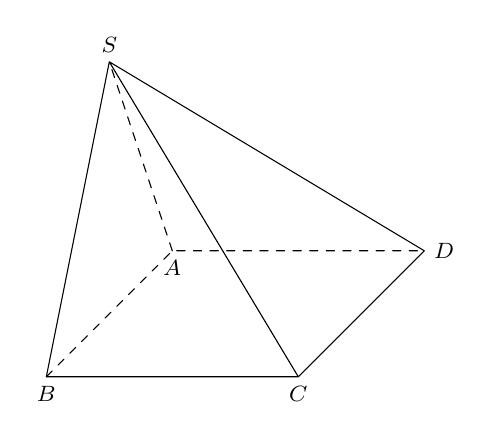
\begin{tikzpicture}[scale=0.8,font=\footnotesize,line join=round,line cap=round,>=stealth]
				\coordinate (a) at (2,2); 
				\coordinate (b) at  (0,0);
				\coordinate (c) at (4,0); 
				\coordinate  (d) at (6,2);
				\coordinate  (s) at (1,5);
				\draw[dashed] (b) -- (a) --  (d)
					(a) --  (s);
				\draw (s) --  (b) -- (c) -- (d)-- (s) -- (c);
				\draw (2,2)  node[below]{$A$};
				\draw (0,0) node[below]{$B$}; 
				\draw (4,0)  node[below]{$C$};
				\draw  (6,2) node[right]{$D$};
				 \draw (1,5) node[above]{$S$};
			\end{tikzpicture}
	}} 
\end{ex}

% nguồn: Ok_TracNghiemLop11_Lan1
\begin{ex}%[1H8N1-3]%[ma:59e68424]
	\immini{Cho hình  chóp $S.ABCD$ có đáy $ABCD$ là hình bình hành. Góc giữa hai đường thẳng $SD$ và $BC$ bằng
	 \choice
		{Góc giữa hai đường $SD$ thẳng và $CD$} 
		{\True Góc giữa hai đường thẳng $SD$ và  $AD$}
		 {Góc giữa hai đường thẳng $SD$ và $BD$}
		{Góc giữa hai đường  thẳng $SD$ và $SC$}
		}{ 
		{\begin{tikzpicture}[scale=1,font=\footnotesize,line join=round,line cap=round,>=stealth]
		\def\a{2}  \def\b{3} \def\h{2.5}
		 \path
			(0:0) coordinate (A) 
			(0:\b) coordinate  (D)
			(-140:\a) coordinate  (B)
			($(B)+(D)-(A)$) coordinate  (C)
			($(A)+(70:\h)$)  coordinate (S);
		 \draw (D)--(C)--(B)--(S)--(C)
			 (S)--(D);
		\draw[dashed]  (S)--(A)--(B)
			 (A)--(D);
		\foreach \x/\g in  {A/180,B/-90,C/-90,D/0,S/90}
		\fill[black]  (\x) circle (1pt)
			($(\x)+(\g:3mm)$) node{$\x$}; 
	\end{tikzpicture}
		 }
		} 
	\loigiai{ 
		Do $BC \parallel AD$ nên góc giữa hai đường thẳng $SD$ và $BC$  bằng góc giữa hai đường thẳng $SD$ và $AD$.
	} 
\end{ex}

% nguồn: Ok_TracNghiemLop11_Lan1
\begin{ex}%[1H8N1-3]%[ma:aadb24dc]
	Cho hình chóp $SABCD$ có đáy là hình vuông $ABCD$ cạnh $a$ và các cạnh bên bằng $a$. Gọi $M$, $N$ lần  lượt là trung điểm $AD$ và $SD$. Số đo góc $(MN,SC)$ bằng
	\choice 
		{$60^{\circ}$} 
		 {$45^{\circ}$}
		{$30^{\circ}$} 
		 {\True $90^{\circ}$}
	 \loigiai{
	 \immini{
		Tam giác  $SAC$ có $SA=SC=a$ và $AC=a\sqrt{2}$ nên tam giác $SAC$ vuông cân tại $S$. \\
		Ta  có $MN\parallel SA$ nên $(MN,SC)=(SA,SC)=90^{\circ}$.
		 }{
		\begin{tikzpicture}[scale=0.8,font=\footnotesize,line join=round,line cap=round,>=stealth]
				\coordinate (a) at (2,2); 
				\coordinate  (b) at (0,0);
				\coordinate  (c) at (4,0);
				 \coordinate (d) at (6,2);
				\coordinate (o) at ($(a)!0.5!(c)$); 
				\coordinate  (s) at ($(o)+(0,5)$);
				\coordinate (m) at  ($(a)!0.5!(d)$);
				\coordinate  (n) at ($(s)!0.5!(d)$);
				\draw[dashed] (b)  -- (a) -- (d)
					(c) --  (a) -- (s)
					(b) --  (d);
				\draw (s) --  (b) -- (c) -- (d)-- (s) -- (c);
				\draw  (a) node[below]{$A$};
				 \draw (b) node[below]{$B$};
				\draw (c) node[below]{$C$}; 
				 \draw (d) node[right]{$D$};
				 \draw (s) node[above]{$S$};
				\draw  (o) node[above]{$O$};
				 \draw (m) node[below]{$M$};
				\draw (n) node[right]{$N$}; 
				 \draw[dashed] (d)--(m) -- (n);
			\end{tikzpicture}
	}} 
\end{ex}

% nguồn: Ok_TracNghiemLop11_Lan1
\begin{ex}%[1H8N1-3]%[ma:4becdd6a]
	Cho hình lập phương $ABCD.A'B'C'D'$. Số đo góc  tạo bởi hai đường thẳng $BD$ và $AB'$ bằng
	\choice 
		{$90^{\circ}$} 
		{\True  $60^{\circ}$}
		 {$45^{\circ}$}
		{$30^{\circ}$} 
	 \loigiai{
	\immini{ 
		 Ta có $AB'\parallel DC' \Leftrightarrow (BD,AB')=(BD,DC')$. \\
		Tam giác $BDC'$ đều vì  $BD=BC'=DC'$ (các đường chéo hình vuông bằng nhau) nên $\widehat{BDC'}=60^{\circ}$. \\
		Vậy  góc tạo bởi hai đường thẳng $BD$ và $AB'$ bằng $60^{\circ}$.
		 }{
		\begin{tikzpicture}[scale=0.6,font=\footnotesize,line join=round,line cap=round,>=stealth]
				\coordinate  (a) at (2,2);
				\coordinate  (b) at (0,0);
				\coordinate (c) at (5,0); 
				\coordinate (d) at (7,2); 
				\coordinate (a1) at ($(a)+(0,5)$); 
				 \coordinate (b1) at ($(b)+(0,5)$);
				\coordinate (c1)  at ($(c)+(0,5)$);
				\coordinate  (d1) at ($(d)+(0,5)$);
				\draw[dashed] (b) --  (a) -- (d)
					 (a) -- (a1);
				\draw (b) -- (c) -- (d) --  (d1) -- (c1) -- (b1) -- (a1) -- (d1)
					(b) --  (b1)
					 (c) -- (c1);
				 \draw (a) node[below]{$A$};
				 \draw (b) node[below]{$B$};
				\draw  (c) node[below]{$C$};
				\draw (d) node[right]{$D$}; 
				\draw  (a1) node[above]{$A'$};
				\draw (b1)  node[below left]{$B'$};
				\draw (c1) node[below  right]{$C'$};
				\draw (d1) node[right]{$D'$}; 
				\draw[dashed] (b)--  (d)
					(b1) -- (a) -- (d1); 
				\draw (b1)  -- (d1);
			\end{tikzpicture}
		} 
	} 
\end{ex}

% nguồn: Ok_TracNghiemLop11_Lan1
\begin{ex}%[1H8N1-3]%[ma:fe40d33e]
	\immini{ 
	Cho hình lập phương $ABCD.A'B'C'D'$. Góc  giữa hai đường thẳng $AB$ và $BD$ bằng bao nhiêu độ?
	 \choice[2]
		 {$30^{\circ}$}
		 {$60^{\circ}$}
		{\True $45^{\circ}$} 
		{$90^{\circ}$} 
		}{ 
		\begin{tikzpicture}[scale=0.7,font=\footnotesize,line join=round,line cap=round,>=stealth]
				\path 
					 (0,0) coordinate (B)
					 (1,0.8) coordinate (A)
					(4,0) coordinate (C) 
					 ($(C)-(B)+(A)$) coordinate (D)
					 ($(A)+(90:3.5)$) coordinate (A')
					($(B)-(A)+(A')$) coordinate  (B')
					 ($(C)-(A)+(A')$) coordinate (C')
					($(D)-(A)+(A')$) coordinate  (D');
				\draw  (B')--(B)--(C)--(D)--(D')--(A')--(B')--(C')--(D')
					 (C)--(C');
				\draw[dashed]  (A)--(D)
					(A')--(A)--(B)--(D); 
				 \foreach \p/\q in {A/160,B/-135,C/-45,D/0,A'/90,B'/180,C'/-20,D'/0}
				\fill[black] (\p) node[shift={(\q:3mm)}]{$\p$} circle  (1.0pt);
			\end{tikzpicture}
		} 
	 \loigiai{
	Ta có $\triangle ABD$ vuông cân nên  $(AB,BD)=45^{\circ}$.}
\end{ex}

% nguồn: Ok_TracNghiemLop11_Lan1
\begin{ex}%[1H8N1-3]%[ma:097f3dc7]
	 \immini{
	 Cho hình lập phương $ABCD.A'B'C'D'$. Góc giữa hai đường thẳng $AA'$ và $DC'$ bằng
	 \choice
		{Góc giữa  hai đường thẳng $AA'$ và $DD'$}
		{Góc giữa hai đường  thẳng $AA'$ và $D'C'$}
		{Góc giữa  hai đường thẳng $DD'$ và $BB'$}
		{\True Góc giữa hai  đường thẳng $DC'$ và $DD'$}
		 }{
		\begin{tikzpicture}[scale=1,font=\footnotesize,line join=round,line cap=round,>=stealth]
				\def\a{1.6} \def\b{2.6} \def\h{2} \def\g{-120} 
				\path 
					(0:0) coordinate  (A)
					(\g:\a)  coordinate (B)
					(0:\b)  coordinate (D)
					($(B)+(D)-(A)$) coordinate  (C);
				\foreach \x in {A,B,C,D} \coordinate (\x') at  ($(\x)+(90:\h)$);
				\draw  (B')--(A')--(D')--(C')--(B')--(B)--(C)--(D)--(D')
					(C)--(C'); 
				 \draw[dashed] (B)--(A)--(D)
					 (A)--(A');
				 \foreach \i/\g in {A/-80,B/-90,C/-90,D/0,A'/90,D'/90,B'/180,C'/110}
				\fill[black] (\i) circle (1pt) 
					 ($(\i)+(\g:3mm)$) node{$\i$};
			\end{tikzpicture}
		} 
	 \loigiai{
	Do $AA' \parallel DD'$ nên góc giữa hai đường thẳng $AA'$  và $DC'$ bằng góc giữa hai đường thẳng $DD'$ và $DC'$.}
\end{ex}

% nguồn: Ok_Toan11_TracNghiem_Lan2
\begin{ex}%[1H8H1-3]%[ma:65521a69]
	Cho hình chóp tứ giác đều $S.ABCD$ có đáy là hình vuông $ABCD$ tâm $O$ cạnh $a$, $SO=\dfrac{a\sqrt{2}}{2}$, góc giữa hai  đường thẳng $AB$ và $SD$ là
	 \choice
		 {$120^\circ$}
		 {\True $60^\circ$}
		{$30^\circ$} 
		 {$90^\circ$}
	 \loigiai{
	 \immini{
		Ta có $AB\parallel  CD$, khi đó $\left(AB,SD\right)=\left(CD,SD\right)$.\\
		Lại có $OD=\dfrac{1}{2} BD=\dfrac{a\sqrt{2}}{2}$.\\ 
		 Do đó $SD=\sqrt{SO^2+OD^2}=\sqrt{\dfrac{a^2}{2}+\dfrac{a^2}{2}}=a$.\\
		Suy ra $ SD=SC=CD=a$,  do đó $ \triangle SCD$ đều, nên $ \widehat{SDC}=60^\circ$.\\
		Vậy  $\left(AB,SD\right)=\left(CD,SD\right)=\widehat{SDC}=60^\circ$.
		}{ 
		\begin{tikzpicture}[line join=round,line cap=round]
				 \coordinate (A) at (0,0);
				\coordinate  (B) at (-2,-1.5);
				\coordinate (D) at  (4,0);
				 \coordinate (C) at ($(B)+(D)-(A)$);
				\coordinate (O)  at ($(A)!0.5!(C)$);
				\coordinate  (S) at ($(O)+(0,4)$);
				\draw (S)--(B)--(C)--(D)--(S) 
					(S)--(C); 
				\draw[dashed,thin](S)--(A)--(C) 
					(B)--(D)--(A)--(B) 
					(S)--(O); 
				\pic[draw,thin,angle radius=2mm]  {right angle = S--O--D} pic[draw,thin,angle radius=2mm] {right angle = S--O--A};
				\foreach \i/\g in {S/90,A/180,B/-90,C/-90,D/0,O/-90}{\draw[fill=white](\i)  circle (1pt)
					 ($(\i)+(\g:3mm)$) node[scale=1]{$\i$};}
			\end{tikzpicture}
		 }
	} 
\end{ex}

% nguồn: Ok_Toan11_TracNghiem_Lan2
\begin{ex}%[1H8H1-3]%[ma:0cda49ed]
	Cho hình lăng trụ $ABC.A'B'C'$ có đáy là $ABC$ là tam giác cân tại $A$, $M$ là trung điểm của $BC$. Góc giữa hai đường thẳng  $B'C'$ và $AM$ bằng
	\choice 
		{$60^\circ$} 
		 {$30^\circ$}
		 {$45^\circ$}
		 {\True $90^\circ$}
	 \loigiai{
	 \immini{
		Do tam giác $ABC$ cân tại $A$ và $M$ là trung điểm đoạn $BC$  nên $AM\perp BC$.\\
		Ta có $BC\parallel B'C'$  do đó $\left(B'C',AM\right)=\left(BC,AM\right)=90^\circ$.
		}{ 
		\begin{tikzpicture}[line join=round,line cap=round]
				\coordinate (A) at  (0,0);
				\coordinate (B) at  (2,-1.5);
				\coordinate (C)  at (4,0);
				\coordinate (A') at (1,3); 
				\coordinate (B')  at ($(B)+(A')-(A)$);
				\coordinate (C')  at ($(C)+(A')-(A)$);
				\coordinate  (M) at ($(B)!0.5!(C)$);
				 \draw (A')--(B')--(C')--(C)--(B)--(A)--(A')
					 (B)--(B')
					(A')--(C'); 
				\draw[dashed](M)--(A)--(C) 
					 (B)--(A)--(B);
				\foreach \i/\g in  {A/180,B/-90,C/-90,A'/90,B'/90,C'/0,M/-90}{
					\fill (\i) circle  (1pt)
					($(\i)+(\g:3mm)$)  node[scale=1]{$\i$};
				 }
			\end{tikzpicture}
		} 
	 }
\end{ex}

% nguồn: Ok_Toan11_TracNghiem_Lan2
\begin{ex}%[1H8H1-3]%[ma:f383f9bc]
	Cho hình chóp $S.ABCD$  có đáy $ABCD$ là hình vuông cạnh $a$, tam giác $SAD$ đều. Góc giữa $BC$ và $SA$ bằng
	 \choice
		{\True  $60^\circ$}
		{$30^\circ$} 
		{$90^\circ$} 
		{$45^\circ$} 
	\loigiai{ 
	\immini{ 
		Vì $BC\parallel  AD\Rightarrow \widehat{\left(BC,SA\right)}=\widehat{\left(AD,SA\right)}=\widehat{SAD}=60^\circ$.
		 }{
		\begin{tikzpicture}[line join=round,line cap=round]
				\coordinate (A) at (0,0); 
				\coordinate (B)  at (5,0);
				\coordinate (D)  at (-2,-1.5);
				\coordinate  (C) at ($(B)+(D)-(A)$);
				\coordinate  (O) at ($(A)!0.5!(D)$);
				 \coordinate (S) at ($(O)+(0,4)$);
				 \draw (S)--(D)--(C)--(B)--(S)
					(S)--(C) 
					 (B)--(C);
				\draw[dashed,thin] (S)--(A)--(D) 
					(S)--(O) 
					(A)--(B); 
				\pic[draw,thin,angle radius=2mm] {right angle = S--O--A}; 
				\foreach  \i/\g in {S/90,A/45,B/-90,C/-90,D/-90,O/-60}{\draw[fill=white](\i) circle (1pt)
					($(\i)+(\g:3mm)$) node[scale=1]{$\i$};} 
			\end{tikzpicture}
		} 
	 }
\end{ex}

% nguồn: Ok_Toan11_TracNghiem_Lan2
\begin{ex}%[1H8H1-3]%[ma:c1f018ba]
	Cho tứ diện $ABCD$ với đáy $BCD$ là tam giác vuông cân tại $C$. Các điểm $M$, $N$, $P$, $Q$ lần lượt là trung  điểm của $AB$, $AC$, $BC$, $CD$. Góc giữa $MN$ và $PQ$ bằng
	 \choice
		{\True  $45^\circ$}
		{$60^\circ$} 
		{$30^\circ$} 
		{$0^\circ$} 
	\loigiai{ 
	 \immini{
		Do $MN$ song song $BC$ và $PQ$  song song $BD$ nên góc giữa $MN$ và $PQ$ bằng góc giữa $BC$ và $BD$ và bằng góc $\widehat{CBD}=45^\circ$.
		}{ 
		\begin{tikzpicture}[line join=round,line cap=round]
				\coordinate (A) at (0,4); 
				\coordinate (B) at  (-2,0);
				\coordinate (C)  at (0,-2);
				\coordinate (D) at  (3,0);
				\coordinate (M) at ($(A)!0.5!(B)$); 
				\coordinate (N)  at ($(A)!0.5!(C)$);
				\coordinate (P) at  ($(B)!0.5!(C)$);
				\coordinate  (Q) at ($(C)!0.5!(D)$);
				\draw (A)--(B)--(C)--(D)--(A) 
					(A)--(C) 
					(M)--(N); 
				\draw[dashed,thin](B)--(D) 
					(P)--(Q); 
				\foreach \i/\g in {A/90,B/180,C/-90,D/0,M/120,N/0,P/-90,Q/-90}{\draw[fill=white](\i) circle (1pt) 
					 ($(\i)+(\g:3mm)$) node[scale=1]{$\i$};}
			\end{tikzpicture}
		} 
	 }
\end{ex}

% nguồn: Ok_TracNghiemLop11_Lan1
\begin{ex}%[1H8H1-3]%[ma:67ee4342]
	 \immini{
	Cho hình chóp $S.ABCD$ có tất cả các cạnh bằng  nhau (hình vẽ minh hoạ). Số đo góc giữa hai đường thẳng $SA$ và $BC$ bằng
	 \choice
		{$90^\circ$} 
		{\True $60^\circ$} 
		{$45^\circ$} 
		{$30^\circ$} 
		}{ 
		\begin{tikzpicture}[scale=1,font=\footnotesize,line join=round,line cap=round,>=stealth]
				\def\a{2} \def\b{3} \def\h{2.5} 
				 \path
					(0:0)  coordinate (A)
					(0:\b) coordinate  (D)
					(-140:\a) coordinate  (B)
					 ($(B)+(D)-(A)$) coordinate (C)
					($(A)+(70:\h)$) coordinate (S); 
				\draw  (D)--(C)--(B)--(S)--(C)
					 (S)--(D);
				 \draw[dashed] (S)--(A)--(B)
					 (A)--(D);
				 \foreach \x/\g in {A/180,B/-90,C/-90,D/0,S/90}
				\fill[black] (\x) circle  (1pt)
					($(\x)+(\g:3mm)$)  node{$\x$};
			\end{tikzpicture}
		 }
	\loigiai{ 
		$S.ABCD$ có tất cả các cạnh bằng nhau suy ra $\triangle SAD$  đều.\\
		Khi đó $BC  \parallel AD$ $\Rightarrow$ $(SA;BC)=(SA;AD)=\widehat{SAD}=60^\circ$
	} 
\end{ex}

% nguồn: Ok_TracNghiemLop11_Lan1
\begin{ex}%[1H8H1-3]%[ma:31eea4b4]
	Cho tứ diện $ABCD$ có $AB = CD = 2a$. Gọi $M$, $N$ lần lượt là trung điểm của $AD$  và $BC$. Biết $MN = \sqrt{3}a$, góc giữa hai đường thẳng $AB$ và $CD$ bằng
	 \choice
		 {$45^{\circ}$}
		 {$90^{\circ}$}
		{\True $60^{\circ}$} 
		 {$30^{\circ}$}
	\loigiai{ 
	 \immini
		{ 
		 Gọi $P$ là trung điểm của $AC$.\\
		Khi đó, ta có\\ 
		$PM\parallel CD$, $PN\parallel AB$.\\ 
		Suy ra góc  giữa $AB$ và $CD$ bằng góc giữa $PM$ và $PN$.\\
		Ta  có $PM=\dfrac{CD}{2}=\dfrac{a}{2},PN=\dfrac{AB}{2}=\dfrac{a}{2}$.\\
		Xét  tam giác $PMN$ có
		\begin{eqnarray*}
			& \cos\widehat{MPN} &  =\dfrac{PM^2+PN^2-MN^2}{2\cdot PM\cdot PN}\\
			&  & =\dfrac{\dfrac{a^2}{4}+\dfrac{a^2}{4}-\dfrac{3a^2}{4}}{2\cdot\dfrac{a}{2}\cdot\dfrac{a}{2}}\\
			& & =-\dfrac{1}{2}. 
		\end{eqnarray*}
		Suy  ra $\widehat{MPN}=120^{\circ}$.\\
		Suy ra $(PM,PN)=180^{\circ}-120^{\circ}=60^{\circ}$.  \\
		Vậy góc giữa hai đường thẳng $AB$ và $CD$  bằng $60^{\circ}$.
		 }{
		\begin{tikzpicture}[>=stealth]
				\tkzDefPoint  (0,0){B}
				\tkzDefShiftPoint[B](0:5){D} 
				\tkzDefShiftPoint[B](-60:2){C} 
				\tkzDefShiftPoint[B](60:4){A} 
				\tkzDefMidPoint (A,D) \tkzGetPoint{M} 
				\tkzDefMidPoint (B,C) \tkzGetPoint{N} 
				\tkzDefMidPoint (A,C) \tkzGetPoint{P} 
				\tkzDrawSegments (A,B A,C A,D  B,C C,D N,P M,P)
				\tkzDrawSegments[dashed](B,D  M,N)
				 \tkzLabelPoint[above](A){\footnotesize $A$}
				\tkzLabelPoint[left](B){\footnotesize  $B$}
				\tkzLabelPoint[left](C){\footnotesize  $C$}
				\tkzLabelPoint[right](D){\footnotesize $D$} 
				\tkzLabelPoint[right](M){\footnotesize $M$} 
				\tkzLabelPoint[left](N){\footnotesize $N$} 
				\tkzLabelPoint[left](P){\footnotesize  $P$}
				 \tkzDrawPoints[fill](A,B,C,D,M,N,P)
			\end{tikzpicture}
		} 
	 }
\end{ex}

% nguồn: Ok_TracNghiemLop11_Lan1
\begin{ex}%[1H8H1-3]%[ma:0149942a]
	Cho hình chóp $SABCD$ có tất cả các cạnh đều bằng $a$. Gọi  $I$ và $J$ lần lượt là trung điểm của $SC$ và $BC$. Số đo góc $(IJ,CD)$ bằng
	 \choice
		{\True $60^{\circ}$} 
		 {$45^{\circ}$}
		{$30^{\circ}$} 
		 {$90^{\circ}$}
	\loigiai{ 
	\immini{ 
		Gọi $O$ là tâm của hình vuông $ABCD$, ta có $OJ \parallel  CD$.\\ $\Rightarrow (IJ,CD)=(IJ,OJ)$. \\
		Tam giác $OIJ$  có $IJ=OJ=OI=\dfrac{SB}{2}=\dfrac{a}{2}$ nên tam giác $OIJ$ đều. \\
		Vậy  $(IJ,CD)=(IJ,OJ)=60^{\circ}$.
		 }{
		\begin{tikzpicture}[scale=0.7,font=\footnotesize,line join=round,line cap=round,>=stealth]
				\coordinate (a) at  (2,2);
				\coordinate  (b) at (0,0);
				\coordinate (c) at  (4,0);
				\coordinate (d) at (6,2); 
				\coordinate  (o) at ($(a)!0.5!(c)$);
				\coordinate (s) at ($(o)+(0,5)$); 
				\coordinate (i)  at ($(s)!0.5!(c)$);
				\coordinate (j) at  ($(c)!0.5!(b)$);
				 \draw[dashed] (b) -- (a) -- (d)
					 (c) -- (a) -- (s)
					(b)  -- (d);
				\draw (s) -- (b) --  (c) -- (d)-- (s) -- (c);
				\draw  (a) node[below]{$A$};
				\draw (b) node[below]{$B$}; 
				\draw (c)  node[below]{$C$};
				\draw  (d) node[right]{$D$};
				\draw  (s) node[above]{$S$};
				 \draw (o) node[above]{$O$};
				\draw  (i) node[left]{$I$};
				\draw  (j) node[below]{$J$};
				\draw (i) -- (j); 
				 \draw[dashed] (i)--(o) -- (j);
			\end{tikzpicture}
		} 
	} 
\end{ex}

% nguồn: Ok_TracNghiemLop11_Lan1
\begin{ex}%[1H8H1-3]%[ma:9e65c1d0]
	Cho hình chóp $S. ABCD$ có đáy là hình bình hành. Góc giữa  hai đường thẳng $SD$ và $BC$ bằng góc nào trong các góc dưới đây?
	\choice 
		{$(SD,  AB)$}
		{\True $(SD,  AD)$}
		 {$(SC, BC)$}
		{$(SB,  BC)$}
	 \loigiai{
	\immini{ 
		Ta có $BC\parallel  AD$ suy ra $(SD,BC)=(SD,AD)$.
		 }
		{\begin{tikzpicture}
		\def\a{3} 
		\path (0:0) coordinate  (A)
			++(0:\a) coordinate (D) 
			++(-130:\a/2) coordinate  (C)
			 ($(A)+(C)-(D)$) coordinate (B)
			($(A)+(80:\a)$) coordinate (S) 
			(intersection of A--C and  B--D) coordinate (O);
		\draw[dashed]  (B)--(A)--(D)
			 (A)--(S);
		\draw (B)--  (C)--(D)
			 (B)--(S)
			(C)--(S) 
			(D)--(S); 
		\foreach \x/\g  in {A/135,B/-135,C/-45,D/45,S/90}
		\fill[black]  (\x) circle (1pt)
			($(\g:3mm)+(\x)$)  node {$\x$};
	\end{tikzpicture}
		} 
	 }
\end{ex}

% nguồn: Ok_TracNghiemLop11_Lan1
\begin{ex}%[1H8H1-3]%[ma:cfa6679a]
	 \immini{
	Cho hình chóp $S. ABC D$ có tất  cả các cạnh bằng nhau. Số đo góc giữa hai đường thẳng $SA$ và $CB$ bằng
	\choice 
		{$45^{\circ}$} 
		 {$30^{\circ}$}
		{\True  $60^{\circ}$}
		 {$90^{\circ}$}
		}{ 
		\begin{tikzpicture}[scale=0.7,font=\footnotesize,line join=round,line cap=round,>=stealth]
				\path (0,0)  coordinate (A)++(0:3) coordinate (D)
					($(A)+(-140:2)$) coordinate (B) 
					 ($(B)+(D)-(A)$) coordinate (C)
					($(B)!1/2!(D)$) coordinate  (O)
					($(O)+(90:3)$) coordinate  (S);
				 \draw (S)--(D)
					 (S)--(C)
					 (S)--(B)
					 (D)--(C)--(B);
				\draw[dashed] (S)--(A) 
					 (B)--(A)--(D);
				\foreach \x/\g in {A/-60,D/0,C/-90,B/-150,S/100} \fill (\x)  circle (1.2pt)+(\g:.3) node[scale=0.8] {$\x$};
			\end{tikzpicture}
		} 
	\loigiai{ 
		 Vì tứ giác $ABCD$ có các cạnh bằng nhau nên $ABCD$ là hình thoi. Suy ra $CB \parallel AD$.\\
		Do vậy, góc giữa hai đường thẳng $SA$ và $CB$ bằng góc giữa hai đường  thẳng $SA$ và $AD$.\\
		Mặt khác $\triangle SAD$ đều (vì các cạnh bằng nhau) nên  góc giữa hai đường thẳng $SA$ và $AD$ bằng $60^\circ$.
	} 
\end{ex}

% nguồn: Ok_TracNghiemLop11_Lan1
\begin{ex}%[1H8H1-3]%[ma:f98b8847]
	Cho hình chóp $SABCD$ có tất cả các cạnh đều bằng $a$ và $O$ là tâm hình vuông $ABCD$. Gọi $M$ là trung điểm $AB$, $N$ là trung điểm $SB$. Gọi $\alpha$ là góc giữa hai đường thẳng $MN$ và $MO$. Khi đó  $\cos \alpha$ bằng
	\choice 
		{$\dfrac{\sqrt{3}}{2}$} 
		 {\True $\dfrac{1}{2}$}
		{$\dfrac{\sqrt{2}}{2}$} 
		{$\dfrac{\sqrt{3}}{6}$} 
	\loigiai{ 
	\immini{ 
		Ta có hình  chóp đều có tất cả các cạnh đều bằng $a$ suy ra tam giác $SAD$ đều và $(SA,AD)=60^{\circ}$. \\
		Mặt khác do  $SA\parallel MN$ và $AD \parallel MO$ nên $\alpha=(MN,MO)=(SA,AD)=60^{\circ}$ $\Rightarrow \cos \alpha =\dfrac{1}{2}$.
		 }{
		\begin{tikzpicture}[scale=0.8,font=\footnotesize,line join=round,line cap=round,>=stealth]
				\coordinate (a) at  (2,2);
				\coordinate  (b) at (0,0);
				\coordinate (c)  at (4,0);
				 \coordinate (d) at (6,2);
				\coordinate (o) at ($(a)!0.5!(c)$); 
				\coordinate (s) at  ($(o)+(0,5)$);
				\coordinate  (m) at ($(a)!0.5!(b)$);
				 \coordinate (n) at ($(s)!0.5!(b)$);
				\draw[dashed] (b) -- (a)  -- (d)
					(c)  -- (a) -- (s)
					(b)  -- (d)
					(n)--(m)--(o); 
				\draw (s) -- (b)  -- (c) -- (d)-- (s) -- (c);
				\draw (a) node[below]{$A$}; 
				\draw  (b) node[below]{$B$};
				\draw (c) node[below]{$C$}; 
				\draw (d)  node[right]{$D$};
				\draw  (s) node[above]{$S$};
				\draw (o) node[above]{$O$}; 
				\draw (m)  node[left]{$M$};
				\draw (n) node[above left]{$N$}; 
			\end{tikzpicture}
		} 
	} 
\end{ex}

% nguồn: Ok_TracNghiemLop11_Lan1
\begin{ex}%[1H8H1-3]%[ma:92950899]
	 Cho tứ diện $ABCD$ có tất cả các cạnh bằng $a$. Gọi $M$ là trung điểm $BC$ và $N$ là trung điểm $AB$. Gọi $\alpha$ là góc giữa hai đường thẳng $DM$ và $MN$
	 \choice
		 {$\dfrac{\sqrt{3}}{2}$}
		{$\dfrac{1}{2}$} 
		{$\dfrac{\sqrt{2}}{2}$} 
		 {\True $\dfrac{\sqrt{3}}{6}$}
	 \loigiai{
	 \immini{
		Có  $MN=\dfrac{AC}{2}=\dfrac{a}{2}$. \\
		$\cos  DMN=\dfrac{DM^2+MN^2-ND^2}{2DM.MN}=\dfrac{\sqrt{3}}{6}$. \\
		Suy ra $\cos  \alpha=\cos (DM,MN)=\dfrac{\sqrt{3}}{6}$.
		 }{
		\begin{tikzpicture}[scale=0.7,font=\footnotesize,line join=round,line cap=round,>=stealth]
				\coordinate (a) at  (2,2);
				\coordinate (b) at  (0,0);
				\coordinate  (c) at (4,0);
				 \coordinate (d) at (6,2);
				\coordinate (o)  at ($(a)!0.5!(c)$);
				\coordinate (s) at  ($(o)+(0,5)$);
				\coordinate  (m) at ($(b)!0.5!(c)$);
				\coordinate (n) at ($(a)!0.5!(b)$); 
				\draw[dashed] (b)  -- (a) -- (d)
					(c)  -- (a) -- (s)
					(b)  -- (d);
				\draw (s) -- (b) --  (c) -- (d)-- (s) -- (c);
				\draw (a) node[below]{$A$}; 
				 \draw (b) node[below]{$B$};
				\draw (c)  node[below]{$C$};
				\draw  (d) node[right]{$D$};
				\draw (s) node[above]{$S$}; 
				 \draw (o) node[above]{$O$};
				\draw (m) node[below]{$M$}; 
				 \draw (n) node[right]{$N$};
				\draw[dashed]  (d)--(m) -- (n);
			\end{tikzpicture}
		 }
	} 
\end{ex}

% nguồn: Ok_TracNghiemLop11_Lan1
\begin{ex}%[1H8H1-3]%[ma:3add7993]
	Cho hình chóp $S . A B C D$ có tất cả các canh đều bằng $a$. Gọi $I$ và $J$ lần lượt là trung điểm của  $S C$ và $B C$. Số đo của góc $(I J, C D)$ bằng
	 \choice
		 {$30^{\circ}$}
		{\True  $60^{\circ}$}
		{$45^{\circ}$} 
		{$90^{\circ}$} 
	 \loigiai{
		\begin{center}
			\begin{tikzpicture}[scale=1,font=\footnotesize,line join=round,line cap=round]
					\foreach \x\y\t  in {0/0/A,-2/-2/B,3/-2/C,1.5/3/S}
					 \coordinate (\t) at (\x,\y);
					\coordinate (D) at ($(A)+(C)-(B)$); 
					\coordinate (O) at  ($(A)!0.5!(C)$);
					\coordinate (I)  at ($(S)!0.5!(C)$);
					\coordinate (J) at ($(C)!0.5!(B)$); 
					 \draw (S)--(B)--(C)--(S)--(D)--(C)
						(I)--(J); 
					\draw[dashed](B)--(A)--(D)--(B) 
						 (S)--(A)--(C);
					\foreach \t/\g in  {S/90,A/160,B/-140,C/-45,D/0,O/-100,I/60,J/-90}
					 \draw[fill] (\t) circle (1pt)
						 node[shift={(\g:7pt)}]{$\t$};
				\end{tikzpicture}
		\end{center}
		Do  $I$, $J$ là trung điểm của $SC$ và $BC$ nên $IJ$ là đường trung bình của tam giác $SBC$.
		 \\
		Suy ra $IJ  \parallel SB $.
		\\ 
		Mặt khác, $CD  \parallel AB $ (do $ABCD$ là hình thoi).
		 \\
		 Khi đó,
		 $$
		\widehat{(IJ,CD)}  = \widehat{(SB,AB)} = \widehat{SBA} = 60^\circ \quad (\triangle SBA \text{ đều.})
		 $$
	} 
\end{ex}

% nguồn: Ok_TracNghiemLop11_Lan1
\begin{ex}%[1H8H1-3]%[ma:dccced40]
	 \immini{
	Cho hình lập phương $ABCD.A'B'C'D'$ (tham khảo  hình vẽ).
	Góc giữa hai  đường thẳng $A'B'$ và $A C$ bằng
	 \choice
		 {\True $45^{\circ}$}{$90^{\circ}$}{$30^{\circ}$}{$60^{\circ}$} }
		{\begin{tikzpicture}[scale=.7,font=\footnotesize,line join=round,line cap=round,>=stealth]
		 \def\bc{4}
		 \def\ba{2}
		\def\gocB{35} 
		\coordinate[label=below left:$B$] (B) at  (0,0);
		\coordinate[label=above left:$A$] (A) at (\gocB:\ba); 
		\coordinate[label=below:$C$]  (C) at (\bc,0);
		\coordinate[label=right:$D$] (D) at  ($(C)-(B)+(A)$);
		\coordinate[label=above left:$A'$] (A') at  ($(A)+(90:\bc)$);
		\coordinate[label=left:$B'$]  (B') at ($(B)-(A)+(A')$);
		 \coordinate[label=below right:$C'$] (C') at ($(C)-(A)+(A')$);
		 \coordinate[label=right:$D'$] (D') at ($(D)-(A)+(A')$);
		\draw (B')--(B)--(C)--(D)--(D')--(A')--(B')--(C')--(D') 
			 (C)--(C');
		\draw[dashed] (A')--(A)--(D) 
			(A)--(B); 
		\foreach \diem  in {A,B,C,D,A',B',C',D'} \fill (\diem) circle (1pt);
	\end{tikzpicture}
		} 
	 \loigiai{
		Ta có  $AB\parallel A'B'$ nên $\left( A'B',AC\right)= \left( AB,AC\right)=\widehat{BAC}=45^{\circ}$.
	 }
\end{ex}

% nguồn: Ok_TracNghiemLop11_Lan1
\begin{ex}%[1H8H1-3]%[ma:6cdabfef]
	Cho hình lập phương $ABCD\cdot A^{\prime} B^{\prime} C^{\prime} D^{\prime}$, góc giữa hai  đường thẳng $A^{\prime} B$ và $B^{\prime} C$ là
	\choice 
		 {$90^{\circ}$}
		{\True $60^{\circ}$} 
		 {$30^{\circ}$}
		{$45^{\circ}$} 
	\loigiai{ 
	\immini{Gọi cạnh  hình lập phương là $a$.\\
		Ta có $A^{\prime} B  \parallel D^{\prime} C \Rightarrow \left(A^{\prime} B, B^{\prime}C \right) = \left(D^{\prime} C, B^{\prime}C \right)$.\\
		Mà $D^{\prime}  C = B^{\prime}C = B^{\prime} D^{\prime} =a\sqrt{2} \Rightarrow \triangle{CB^{\prime} D^{\prime}}$ đều hay $\widehat{D^{\prime}CB^{\prime}}= 60^{\circ}$.\\ Suy ra $\left(D^{\prime} C, B^{\prime}C \right) = \widehat{D^{\prime}CB^{\prime}}= 60^{\circ}$.\\
		Vậy góc giữa  hai đường thẳng $A^{\prime} B$ và $B^{\prime} C$ bằng $60^{\circ}.$}{
		\begin{tikzpicture}[scale=0.7,font=\footnotesize,line join=round,line cap=round,>=stealth]
				\def\bc{4} 
				 \def\ba{2}
				\def\h{4} 
				\def\gocB{35} 
				\coordinate[label=below left:$B$] (B) at (0,0); 
				\coordinate[label=above left:$A$]  (A) at (\gocB:\ba);
				\coordinate[label=below:$C$]  (C) at (\bc,0);
				\coordinate[label=right:$D$] (D) at  ($(C)-(B)+(A)$);
				 \coordinate[label=above left:$A'$] (A') at ($(A)+(90:\h)$);
				\coordinate[label=left:$B'$]  (B') at ($(B)-(A)+(A')$);
				 \coordinate[label=above:$C'$] (C') at ($(C)-(A)+(A')$);
				\coordinate[label=right:$D'$] (D') at ($(D)-(A)+(A')$); 
				\draw (D')--(B') 
					 (C)--(B')--(B)--(C)--(D)--(D')--(A')--(B')--(C')--(D')--(C)--(C');
				\draw[dashed]  (B)--(A')--(A)--(D)
					 (A)--(B)
					(A)--(C); 
				\foreach \diem in {A,B,C,D,A',B',C',D'} \fill  (\diem) circle (1pt);
			\end{tikzpicture}
		 }
	} 
\end{ex}

% nguồn: Ok_TracNghiemLop11_Lan1
\begin{ex}%[1H8H1-3]%[ma:909cf2f8]
	\immini{ Cho hình hộp chữ nhật $ABCD.A'B'C'D'$, biết đáy $ABCD$ là hình vuông. Tính góc giữa $AC'$ và  $BD$.
	 \choice
		{$60^{\circ}$} 
		 {$30^{\circ}$}
		{\True $90^{\circ}$} 
		{$45^{\circ}$}}{\begin{tikzpicture}[scale=.7,>=stealth,font=\footnotesize,line join=round,line cap=round]
		\def\a{4} 
		 \def\b{2.5}
		 \def\h{3.5}
		\path (0:0) coordinate  (B)
			++(0:\a) coordinate (C) 
			++(-130:\b) coordinate (D) 
			 ($(B)+(D)-(C)$) coordinate (A)
			($(A)+(90:\h)$)  coordinate (A')
			($(B)+(90:\h)$) coordinate  (B')
			($(C)+(90:\h)$) coordinate (C') 
			($(D)+(90:\h)$) coordinate  (D');
		\draw[dashed]  (A)--(B)--(C)
			 (B)--(B')
			 (A')--(C)
			(B)--(D) 
			 (A)--(C);
		\draw[thick] (C)--(C') 
			 (D)--(D')
			(A)--(A') 
			 (A)--(D)--(C)
			 (A')--(B')--(C')--(D')--cycle;
		\foreach \x/\g  in {A/180,B/180,C/0,D/0,A'/180,B'/180,C'/0,D'/0}
		\fill[black] (\x) circle  (1pt)
			($(\g:4mm)+(\x)$)  node {$\x$};
	\end{tikzpicture}
		} 
	\loigiai{Vì $ABCD$ là hình vuông nên  $BD\perp AC$.\\
		Mặt  khác $AA'\perp (ABCD)\Rightarrow BD\perp AA'$.\\
		Ta có $\heva{&BD\perp AC\\&BD\perp  AA'}\Rightarrow BD\perp (AA'C)\Rightarrow BD\perp A'C$.\\
	Do đó, góc giữa $AC'$  và $BD$ bằng $90^{\circ}$.}
\end{ex}

% nguồn: Ok_TracNghiemLop11_Lan1
\begin{ex}%[1H8H1-3]%[ma:fbeaec56]
	Cho hình lập phương $ABCD. A'B'C'D'$.  Góc giữa hai đường thẳng $BD$ và $AD'$ bằng
	 \choice
		{$30^\circ$} 
		{$45^\circ$} 
		 {\True $60^\circ$}
		{$90^\circ$} 
	\loigiai{\begin{center}
	\begin{tikzpicture}[scale=1,font=\footnotesize,line join=round,line cap=round,>=stealth]
			 \def\bc{4}
			 \def\ba{2}
			\def\gocB{35} 
			\coordinate[label=below left:$B$] (B) at  (0,0);
			\coordinate[label=above left:$A$] (A) at  (\gocB:\ba);
			\coordinate[label=below:$C$] (C)  at (\bc,0);
			\coordinate[label=right:$D$] (D)  at ($(C)-(B)+(A)$);
			\coordinate[label=above left:$A'$] (A')  at ($(A)+(90:\bc)$);
			\coordinate[label=left:$B'$] (B')  at ($(B)-(A)+(A')$);
			\coordinate[label=below right:$C'$] (C')  at ($(C)-(A)+(A')$);
			\coordinate[label=right:$D'$] (D')  at ($(D)-(A)+(A')$);
			\draw (B')--(B)--(C)--(D)--(D')--(A')--(B')--(C')--(D') 
				(C)--(C'); 
			 \draw[dashed] (A')--(A)--(D)
				 (A)--(B)
				(B)--(D) 
				 (A)--(D');
			\foreach  \diem in {A,B,C,D,A',B',C',D'}\fill (\diem) circle (1pt);
		\end{tikzpicture}
\end{center}
Vì $BD \parallel B'D'$ nên góc giữa  hai đường thẳng $BD$ và $AD'$ là góc giữa hai đường thẳng $B'D'$ và $AD'$.\\
Vì  $AB',AD',B'D'$ lần lượt là đường chéo của các hình vuông bằng nhau $ABB'A',ADD'A',A'B'C'D'$ nên $AB'=AD'=B'D'$.\\
Suy ra tam giác  $AB'D'$ là tam giác đều nên $\widehat{AD'B'}=60^{\circ}$.\\
Vậy góc giữa hai đường thẳng $BD$  và $AD'$ bằng $60^{\circ}$.
 }
\end{ex}

% nguồn: Ok_TracNghiemLop11_Lan1
\begin{ex}%[1H8H1-3]%[ma:5b591150]
	Cho tứ diện $A B C D$ có $A B=A  C=2$, $D B=D C=3$. Khẳng định nào sau đây đúng?
	\choice 
		{\True $B C  \perp A D$}
		{$A C \perp B D$} 
		{$A B \perp(B C D)$} 
		{$D C \perp(A  B C)$}
	\loigiai{ 
		Do $A B=A C=2$,  $D B=D C=3$ nên $A$ và $D$ nằm trên mặt phẳng trung trực của $BC$.
		 \\
		Suy  ra $B C \perp A D$.
	 }
\end{ex}

% nguồn: Ok_TracNghiemLop11_Lan1
\begin{ex}%[1H8H1-3]%[ma:2cc7eb1a]
	Cho hình chóp $S.ABCD$ có đáy là hình vuông cạnh $a$,  cạnh bên $SA$ vuông góc với mặt đáy, $SA=a$, gọi $M$ là trung điểm $SB$. Góc giữa $AM$ và $BD$ bằng
	\choice 
		 {$90^\circ$}
		{$30^\circ$} 
		 {\True $60^\circ$}
		 {$45^\circ$}
	 \loigiai{\immini{Gọi $N$ lần lượt là trung điểm của $SD$. Khi đó $MN$ là dường trung bình của tam giác $SBD$. Ta có $$\Rightarrow MN\parallel BD \Rightarrow (AM,BD)=(AM,MN).$$
		Ta có $AM$ và $AN$ lần lượt là đường trung tuyến của  các tam giác vuông $SAB$ và $SAD$ nên $AM=\dfrac{SB}{2}=\dfrac{SD}{2}=AN=\dfrac{a\sqrt{2}}{2}$. Lại có $MN$ là đường trung bình tam giác $SBD$ nên $MN=\dfrac{BD}{2}=\dfrac{a\sqrt{2}}{2}$.\\
		Từ đó suy ra tam  giác $AMN$ đều cạnh $\dfrac{a}{\sqrt{2}}$. Vậy $(AM,MN)=60^\circ$.}
		{\begin{tikzpicture}[>=stealth,line join=round,line cap=round,font=\footnotesize,scale=0.5]
		 \clip (-4,-4) rectangle (9,7);
		 \def\r{6.5};
		 \def\g{120};
		 \def\gC{30};
		\path 
			 (0,0) coordinate (A)
			(-3,-3)  coordinate (B)
			 (5,-3) coordinate (C)
			(8,0)  coordinate (D)
			 (0,6) coordinate (S);
		\draw (S)--(B)--(C)--(D)--(S)--(C); 
		\coordinate (M) at  ($(S)!0.5!(B)$);
		 \coordinate (N) at ($(S)!0.5!(D)$);
		 \draw[dashed] (S)--(A)--(D)
			(B)--(A)--(M) circle (1pt) node[above  left]{$M$}--(N) circle (1pt) node[above right]{$N$}--(A)
			 (B)--(D);
		\fill[black]  (A) circle (1pt) node[below right]{$A$}
			(C) circle (1pt)  node[below right]{$C$}
			 (B) circle (1pt) node[below left]{$B$}
			(D) circle (1pt)  node[above right]{$D$}
			(S) circle (1pt) node[above right]{$S$}; 
		 \draw pic[draw,angle radius = 5pt] {right angle =S--A--B};
		 \draw pic[draw,angle radius = 5pt] {right angle =S--A--D};
	\end{tikzpicture}
		 }
	} 
\end{ex}

% nguồn: Ok_TracNghiemLop11_Lan1
\begin{ex}%[1H8H1-3]%[ma:bc6ac4d1]
	\immini{ Cho hình lập phương $ABCD.A'B'C'D'$. Góc giữa hai đường thẳng  $BA'$ và $CD$ bằng
	\choice 
		 {\True $45^{\circ}$}
		 {$60^{\circ}$}
		 {$30^{\circ}$}
		 {$90^{\circ}$}}{
		\begin{tikzpicture}[scale=.7,>=stealth,font=\footnotesize,line join=round,line cap=round]
				\def\a{3.5} 
				\path  (0:0) coordinate (A)
					++(0:\a) coordinate (D) 
					++(-130:\a/2)  coordinate (C)
					($(A)+(C)-(D)$) coordinate (B) 
					 ($(A)+(90:\a)$) coordinate (A')
					($(B)+(90:\a)$) coordinate  (B')
					($(C)+(90:\a)$) coordinate (C') 
					($(D)+(90:\a)$) coordinate (D'); 
				\draw[dashed] (B)--(A)--(D) 
					(A)--(A') 
					(B)--(A'); 
				\draw[thick] (C)--(C') 
					 (D)--(D')
					(B)--(B') 
					 (B)--(C)--(D)
					(A')--(B')--(C')--(D')--cycle; 
				 \foreach \x/\g in {A/180,B/180,C/0,D/0,A'/180,B'/180,C'/0,D'/0}
				\fill[black]  (\x) circle (1pt)
					 ($(\g:4mm)+(\x)$) node {$\x$};
			\end{tikzpicture}
		 }
	\loigiai{Ta có $CD\parallel  AB$.\\
	$\Rightarrow \left(BA',CD\right)=\left(BA',BA\right)=\widehat{ABA'}=45^{\circ}$  (do $ABB'A$ là hình vuông).}
\end{ex}

% nguồn: Ok_TracNghiemLop11_Lan1
\begin{ex}%[1H8H1-3]%[ma:2bd455a0]
	\immini{Cho hình lập phương $ABC D. A_1 B_1 C_1 D_1$. Góc giữa  hai đường thẳng $AA_1$ và $DC_1$ bằng
	\choice 
		{Góc giữa hai đường thẳng $DD_1$  và $BB_1$}
		{\True Góc giữa hai đường  thẳng $DC_1$ và $DD_1$}
		{Góc giữa hai  đường thẳng $AA_1$ và $D_1 C_1$}
		{Góc giữa hai đường  thẳng $AA_1$ và $DD_1$}
		 }{
		\begin{tikzpicture}[scale=0.7,font=\footnotesize,line join=round,line cap=round,>=stealth]
				\path (0,0) coordinate (A)++(0:3) coordinate  (D)
					($(A)+(-120:2)$) coordinate (B) 
					 ($(B)+(D)-(A)$) coordinate (C)
					($(A)+(90:2)$)  coordinate (A_1)
					($(B)+(90:2)$) coordinate (B_1) 
					 ($(C)+(90:2)$) coordinate (C_1)
					($(D)+(90:2)$)  coordinate (D_1);
				\draw (D_1)--(D) 
					(C_1)--(C) 
					(B_1)--(B) 
					(D)--(C)--(B) 
					 (A_1)--(B_1)--(C_1)--(D_1)--(A_1)
					(D)--(C_1); 
				\draw[dashed] (A_1)--(A) 
					(B)--(A)--(D); 
				\foreach \x/\g in {A/-60,D/0,C/-90,B/-150,B_1/180,A_1/100,C_1/110,D_1/60} \fill (\x) circle (1.2pt)+(\g:.3)  node[scale=0.8] {$\x$};
			\end{tikzpicture}
		} 
	 \loigiai{
		Vì $ABC D. A_1 B_1 C_1 D_1$ là hình lập phương nên $AA_1 \parallel DD_1$.\\ 
		Suy ra góc giữa hai đường thẳng $AA_1$ và $DC_1$  bằng góc giữa hai đường thẳng $DC_1$ và $DD_1$.
	} 
\end{ex}

% nguồn: Ok_TracNghiemLop11_Lan1
\begin{ex}%[1H8H1-3]%[ma:a249c05d]
	Cho hình chóp $S.ABCD$ có đáy $ABCD$ là hình chữ nhật với $AB=2a$, $BC=a$. Các cạnh bên của hình chóp cùng bằng $a\sqrt{2}$. Tính góc giữa hai đường  thẳng $AB$ và $SC$.
	\choice 
		 {\True $45^{\circ}$}
		{$30^{\circ}$} 
		 {$60^{\circ}$}
		{$\alpha$  với $\tan\alpha=2$}
	 \loigiai{
	 \immini{
		Ta có  $AB\parallel CD$ nên $(AB,SC)=(CD,SC)=\widehat{SCD}$.\\
		Gọi $M$ là  trung điểm $CD$, khi đó tam giác $SCM$ vuông tại $M$ (do $SC=SD$).\\
		Khi đó $\cos\widehat{SCD}=\cos\widehat{SCM}=\dfrac{CM}{SC}=\dfrac{a}{a\sqrt{2}}=\dfrac{\sqrt{2}}{2}\Rightarrow \widehat{SCD}=45^{\circ}$.\\ 
		Vậy góc giữa hai đường thẳng  $AB$ và $SC$ bằng $45^{\circ}$.
		 }{
		\begin{tikzpicture}[scale=0.8,font=\footnotesize,line join=round,line cap=round,>=stealth]
				\coordinate (A) at (0,0); 
				\coordinate (B) at (-2,-1.5); 
				\coordinate (D) at  (5,0);
				 \coordinate (C) at ($(B)+(D)-(A)$);
				 \coordinate (O) at ($(A)!0.5!(C)$);
				\coordinate (S) at  ($(O)+(0,4)$);
				\coordinate (M)  at ($(D)!0.5!(C)$);
				\draw (M)--(S)--(B) 
					(C)--(D)--(S)--(C)--(B); 
				\draw[dashed](S)--(A)--(D) 
					 (A)--(B);
				 \pic[draw,angle radius=2mm] {right angle = C--M--S};
				\pic[draw,angle  radius=5mm]{angle=M--C--S};
				\foreach \i/\g  in {S/90,A/180,B/-90,C/-90,D/0,M/-30}{\draw[fill](\i) circle (1.2pt)
					($(\i)+(\g:3mm)$)  node[scale=1]{$\i$};}
			\end{tikzpicture}
		 }
	} 
\end{ex}

% nguồn: Ok_TracNghiemLop11_Lan1
\begin{ex}%[1H8H1-3]%[ma:57ed7e15]
	Cho hình lập phương $ABCD.A'B'C'D'$ cạnh $a$, $M$ là trung điểm $CD$.  Gọi $\alpha$ là góc tạo bởi $A'B$ và $D'M$. Tính $\cos \alpha$.
	\choice 
		{$\cos  \alpha=\dfrac{1}{2}$}
		 {\True $\cos \alpha=\dfrac{3\sqrt{5}}{5}$}
		{$\cos  \alpha=\dfrac{\sqrt{2}}{2}$}
		{$\cos  \alpha=\dfrac{\sqrt{10}}{10}$}
	 \loigiai{
	 \immini{
		Ta có $D'C\parallel A'B$ nên $(A'B,D'M)=(D'C,D'M)=\alpha$. \\ 
		Có $D'M=\dfrac{a\sqrt{5}}{2}$, $D'C=a\sqrt{2}$,  $CM=\dfrac{a}{2}$. \\
		Tam giác  $D'MC$ có $$\cos \alpha=\dfrac{D'M^2+D'C^2-CM^2}{2D'M.D'C}=\dfrac{3\sqrt{5}}{5}.$$
		}{ 
		\begin{tikzpicture}[scale=0.6,font=\footnotesize,line join=round,line cap=round,>=stealth]
				\coordinate (a) at (2,2); 
				\coordinate (b) at  (0,0);
				\coordinate (c) at (5,0); 
				\coordinate (d) at  (7,2);
				\coordinate  (a1) at ($(a)+(0,5)$);
				 \coordinate (b1) at ($(b)+(0,5)$);
				\coordinate  (c1) at ($(c)+(0,5)$);
				\coordinate (d1)  at ($(d)+(0,5)$);
				\coordinate  (m) at ($(c)!0.5!(d)$);
				\draw[dashed] (b) -- (a) -- (d) 
					(a)  -- (a1);
				\draw (b) -- (c) -- (d) -- (d1) -- (c1) -- (b1)  -- (a1) -- (d1)
					(b) --  (b1)
					(c)  -- (c1);
				\draw (a) node[below]{$A$}; 
				\draw  (b) node[below]{$B$};
				\draw (c)  node[below]{$C$};
				\draw (d)  node[right]{$D$};
				\draw (a1) node[above]{$A'$}; 
				\draw  (b1) node[below left]{$B'$};
				\draw (c1) node[below right]{$C'$}; 
				\draw  (d1) node[right]{$D'$};
				\draw (m)  node[right]{$M$};
				 \draw[dashed] (a1)-- (b);
				\draw (m) -- (d1) -- (c); 
			\end{tikzpicture}
		 }
	 }
\end{ex}

% nguồn: Ok_TracNghiemLop11_Lan1
\begin{ex}%[1H8H1-3]%[ma:fb64c473]
	Cho  hình chóp $S.ABCD$ có đáy $ABCD$ là hình bình hành và tam giác $SAD$ vuông cân tại $S$. Góc giữa hai đường thẳng $SA$ và $BC$ bằng
	\choice 
		 {$60^{\circ}$}
		{\True $45^{\circ}$} 
		 {$30^{\circ}$}
		{$90^{\circ}$} 
	 \loigiai{
	 \immini{
		Vì $BC\parallel AD$ và $\Delta SAD$ vuông cân tại  $S$\\
		 nên $\left(BC,SA\right)=(AD,SA)=\widehat{SAD}=45^{\circ}$.
		 }{
		\begin{tikzpicture}[scale=0.6,line cap=round,line join=round,>=stealth,transform shape]
				\path (0,0) coordinate (A) 
					(-2,-2) coordinate (B) 
					 (5,0) coordinate (D)
					(3,-2) coordinate (C) 
					 (1.5,-1) coordinate (O)
					 (2.5,4) coordinate (S);
				 \draw[dashed] (S)--(A)--(B)
					(A)--(D) 
					(A)--(C) 
					 (B)--(D);
				\draw (B)--(C)--(D)--(S)--(B) 
					(S)--(C); 
				\foreach \p/\q in {A/180,B/-90,C/-90,D/0,S/90} 
				\fill[blue]  (\p) circle (1pt) node[shift={(\q:3mm)}]{$\p$};
				\path  pic[draw,angle radius=5pt]{right angle= A--S--D};
			\end{tikzpicture}
		} 
	 }
\end{ex}

% nguồn: Ok_Toan11_TracNghiem_Lan2
\begin{ex}%[1H8V1-3]%[ma:5cc07f20]
	 Cho hình chóp $S.ABC$ có độ dài các cạnh $SA=SB=SC=AB=AC=a$ và $BC=a\sqrt{2}$. Góc giữa hai đường thẳng $AB$ và $SC$ là?
	 \choice
		 {\True $60^\circ$}
		 {$90^\circ$}
		 {$30^\circ$}
		 {$45^\circ$}
	\loigiai{ 
		\begin{center}
			\begin{tikzpicture}[line join=round,line cap=round]
					\coordinate (B)  at (-2,0);
					\coordinate (A)  at (1.5,-2.5);
					\coordinate (C)  at (3,0);
					\coordinate (N) at  ($(A)!0.5!(C)$);
					 \coordinate (M) at ($(B)!0.5!(C)$);
					\coordinate  (S) at ($(M)+(0,4)$);
					 \coordinate (I) at ($(S)!0.5!(B)$);
					 \draw (S)--(B)--(A)--(C)--(S)
						(S)--(A) 
						 (S)--(N);
					 \draw[dashed,thin](S)--(M)--(N)--(I)--(M)
						 (N)--(B)--(C);
					\pic[draw,thin,angle radius=2mm] {right angle = B--A--C} pic[draw,thin,angle radius=2mm] {right angle =  S--N--C};
					\foreach  \i/\g in {S/90,A/-90,B/180,C/0,M/-90,N/0,I/180}{\draw[fill=white](\i) circle (1pt)
						 ($(\i)+(\g:3mm)$) node[scale=1]{$\i$};}
				\end{tikzpicture}
		\end{center}
		Ta có $BC^2=AB^2+AC^2\Rightarrow \triangle ABC$ vuông tại  $A$.\\
		 Suy ra trung điểm $M$ của cạnh huyền $BC$ là tâm đường tròn ngoại tiếp tam giác $ABC$.\\
		Vì $SA=SB=SC$ nên $SM$ là đường  cao của hình chóp $S.ABC$.\\
		Gọi $N$, $I$ lần lượt là trung điểm của $AC$, $SB$.\\ 
		Ta có $MN\parallel AB$ và $IM\parallel SC$ nên $\left(\widehat{SC,AB}\right)=\left(\widehat{IM,MN}\right)$.\\ 
		Mặt khác 
		 \[BN=\sqrt{AB^2+AN^2}=\sqrt{a^2+\dfrac{a^2}{4}}=\dfrac{a\sqrt{5}}{2}.\]
		\[SN=\sqrt{SC^2-NC^2}=\sqrt{a^2-\dfrac{a^2}{4}}=\dfrac{a\sqrt{3}}{2}.\] 
		\[NI=\dfrac{\sqrt{2\left(BN^2+SN^2\right)-SB^2}}{2}=\dfrac{\sqrt{2\left(\dfrac{5a^2}{4}+\dfrac{3a^2}{4}  \right)-a^2}}{2}=\dfrac{a\sqrt{3}}{2}.\]
		 \[MN=\dfrac{a}{2},~ MI=\dfrac{a}{2}.\]
		Xét tam giác $IMN$, ta có 
		\[\cos \widehat{NMI}=\dfrac{MN^2+IM^2-IN^2}{2\cdot  MN\cdot IM}=\dfrac{\dfrac{a^2}{4}+\dfrac{a^2}{4}-\dfrac{3a^2}{4}}{2\cdot \dfrac{a}{2} \cdot \dfrac{a}{2}}=-\dfrac{1}{2} \Rightarrow \widehat{NMI}=120^\circ.\]
		Suy ra $\left(\widehat{IM,MN}\right)=60^\circ$. 
	 }
\end{ex}

% nguồn: Ok_Toan11_TracNghiem_Lan2
\begin{ex}%[1H8V1-3]%[ma:4d028edb]
	Cho hình hộp $ABCD.A'B'C'D'$ có độ dài tất cả các  cạnh bằng $a$ và các góc $\widehat{BAD}$, $\widehat{DAA'}$, $\widehat{A'AB}$ đều bằng $60^\circ$. Gọi $M$, $N$ lần lượt là trung điểm của $AA'$, $CD$. Gọi $\alpha$ là góc tạo bởi hai đường thẳng $MN$ và $B'C$, giá trị của $\cos \alpha$ bằng
	 \choice
		 {$\dfrac{2}{\sqrt{5}}$}
		{$\dfrac{1}{\sqrt{5}}$} 
		{$\dfrac{3}{\sqrt{5}}$} 
		 {\True $\dfrac{3\sqrt{5}}{10}$}
	\loigiai{ 
		\begin{center}
			\begin{tikzpicture}[line join=round,line cap=round]
					\coordinate  (A') at (0,0);
					\coordinate  (B') at (5,0);
					\coordinate (D') at (3.5,1.5); 
					\coordinate  (C') at ($(B')+(D')-(A')$);
					\coordinate (A)  at ($(A')+(-1,4)$);
					\coordinate (B) at  ($(B')+(A)-(A')$);
					 \coordinate (D) at ($(D')+(A)-(A')$);
					\coordinate (C) at ($(C')+(A)-(A')$); 
					\coordinate  (M) at ($(A)!0.5!(A')$);
					\coordinate (N) at  ($(D)!0.5!(C)$);
					 \coordinate (P) at ($(D)!0.5!(C')$);
					\draw (A)--(D)--(C)--(B)--(A)--(A')--(B')--(C')--(C)--(B')--(B); 
					\draw[dashed,thin] (D)--(A')--(C')--(D)--(D')--(A') 
						 (D')--(C')
						 (M)--(N)
						 (A')--(P);
					\foreach \i/\g in {A'/-90,B'/-90,C'/0,D'/-90,A/180,B/120,C/0,D/90,M/180,N/90,P/60}{\draw[fill=white](\i) circle  (1pt)
						 ($(\i)+(\g:3mm)$) node[scale=1]{$\i$};}
				\end{tikzpicture}
		\end{center}
		Gọi $P$ là  trung điểm của $DC'$.\\
		Ta có $\heva{&A'D\parallel B'C \\ &MN\parallel A'P}$. Suy ra $\widehat{\left(MN,B'C\right)}=\widehat{\left(A'P,A'D\right)}=\widehat{DA'P}=\alpha$.\\ 
		$\triangle ADA'$ có $AD=AA'$ và $\widehat{DAA'}=60^\circ$ nên $\triangle ADA'$  là tam giác đều.\\
		 Suy ra $A'D=a$.
		$\Delta A'AB$ có $AB=AA'$ và  $\widehat{A'AB}=60^\circ$ nên $\Delta A'AB$ là tam giác đều.\\
		Do đó $\triangle D'DC$ cũng là tam  giác đều. Vậy $DC'=2DP=2.\dfrac{a\sqrt{3}}{2}=a\sqrt{3}$.\\
		$\triangle BAD$ có $AD=AB$ và $\widehat{BAD}=60^\circ$ nên $\triangle BAD$ là tam giác  đều.\\
		Vì $\triangle BAD$ là tam giác đều nên $\triangle  B'A'D'$ cũng là tam giác đều.\\
		Gọi $A'I$ là đường cao của $\Delta B'A'D'$.  Khi đó $A'C'=2A'I=2\dfrac{a\sqrt{3}}{2}=a\sqrt{3}$.\\
		Ta có $A'P$ là đường trung tuyến của tam giác  $DA'C'$ nên \[A'P=\dfrac{A'D^2+A'C'^2}{2}-\dfrac{DC'^2}{4}=\dfrac{\sqrt{5} a}{2}.\]
		Áp dụng định lý cosin cho  tam giác $A'DP$, ta có
		\[\cos  \alpha=\dfrac{A'D^2+A'P^2-DP^2}{2\cdot A'D\cdot A'P}=\dfrac{3\sqrt{5}}{10}.\]
	 }
\end{ex}

% nguồn: Ok_Toan11_TracNghiem_Lan2
\begin{ex}%[1H8V1-3]%[ma:d87a1a78]
	Cho hình chóp $S.ABCD$ có đáy $ABCD$ là hình vuông, cạnh bên $SA$ vuông góc với mặt phẳng đáy,  $SA=AB=a$. Gọi $M$ là trung điểm của $SB$. Góc giữa $AM$ và $BD$ bằng
	\choice 
		 {$45^\circ$}
		 {$30^\circ$}
		 {$90^\circ$}
		{\True $60^\circ$} 
	\loigiai{ 
		\begin{center}
			\begin{tikzpicture}[line join=round,line cap=round]
					\coordinate (A) at  (0,0);
					\coordinate (D) at  (-3,-3);
					\coordinate (B)  at (6,0);
					 \coordinate (C) at ($(B)+(D)-(A)$);
					\coordinate  (S) at ($(A)+(0,5)$);
					\coordinate (M) at  ($(S)!0.5!(B)$);
					\coordinate (E)  at ($(M)!0.5!(C)$);
					\coordinate (O) at  ($(A)!0.5!(C)$);
					\draw  (S)--(B)--(E)
						(S)--(C)--(M) 
						 (S)--(D)
						 (B)--(C)--(D);
					 \draw[dashed,thin](S)--(A)--(D)--(B)--(A)--(C)
						(A)--(M) 
						(D)--(E)--(O); 
					\pic[draw,thin,angle radius=6pt] {right angle = S--A--D} pic[draw,thin,angle radius=6pt] {right angle  = S--A--B};
					\foreach \i/\g in  {S/90,A/-90,B/0,C/-90,D/-90,M/45,O/-90,E/-45}{\draw[fill=white](\i) circle (1pt)
						($(\i)+(\g:3mm)$)  node[scale=1]{$\i$};}
				\end{tikzpicture}
		\end{center}
		 Xét tam giác $SAB$ vuông tại $A$ có $SB=\sqrt{SA^2+AB^2}=a\sqrt{2}$.\\
		Gọi $E$ là trung điểm của  $MC$, ta có $OE\parallel AM$. \\
		Suy ra $\left(\widehat{AM,BD}\right)=\left(\widehat{OE,BD}\right)$ và $OE=\dfrac{1}{2}  AM=\dfrac{1}{4} SB=\dfrac{a\sqrt{2}}{4}$.\\
		 Ta có $CB\perp AB,SA\perp CB\Rightarrow CB\perp SB\Rightarrow \triangle SBC$ vuông tại $B$.\\
		Xét  tam giác $MBC$ vuông tại $B$ có $MC=\sqrt{MB^2+BC^2}=\sqrt{\dfrac{1}{4}\cdot2a^2+a^2}=\dfrac{a\sqrt{6}}{2}$\\ và $BE=\dfrac{1}{2} MC=\dfrac{a\sqrt{6}}{4}$.\\
		Xét tam giác $BCD$ vuông tại $C$  có $BD=\sqrt{BC^2+DC^2}=a\sqrt{2} \Rightarrow BO=\dfrac{a\sqrt{2}}{2}$.\\
		Xét tam giác $EBO$  có $\cos \widehat{EOB}=\dfrac{EO^2+OB^2-EB^2}{2\cdot EO\cdot OE}=\dfrac{\dfrac{a^2}{8}+\dfrac{a^2}{2}-\dfrac{3a^2}{8}}{2\cdot\dfrac{a\sqrt{2}}{4}\cdot\dfrac{a\sqrt{2}}{2}}=\dfrac{1}{2} \Rightarrow \widehat{EOB}=60^\circ$.\\
		Vậy $\left(\widehat{AM,BD}\right)=\left(\widehat{OE,BD}\right)=\widehat{EOB}=60^\circ$. 
	} 
\end{ex}

% nguồn: Ok_Toan11_TracNghiem_Lan2
\begin{ex}%[1H8V1-3]%[ma:550afa5b]
	Cho hình chóp $S.ABCD$ có đáy hình vuông, tam giác $SAB$ vuông tại $S$ và $\widehat{SBA}=30^\circ$. Mặt phẳng $\left(SAB\right)$ vuông góc với mặt phẳng đáy. Gọi $M$ là trung điểm của $AB$. Tính cosin góc tạo bởi hai  đường thẳng $\left(SM,BD\right)$.
	\choice 
		 {$\dfrac{1}{\sqrt{3}}$}
		 {$\dfrac{\sqrt{2}}{\sqrt{3}}$}
		{$\dfrac{\sqrt{26}}{13}$} 
		{\True $\dfrac{\sqrt{2}}{4}$} 
	\loigiai{ 
		\begin{center}
			\begin{tikzpicture}[line join=round,line cap=round]
					 \coordinate (A) at (0,0);
					\coordinate (D)  at (6,0);
					\coordinate (B) at (-2,-2.5); 
					 \coordinate (C) at ($(B)+(D)-(A)$);
					\coordinate (M) at ($(A)!0.5!(B)$); 
					 \coordinate (H) at ($(A)!0.5!(M)$);
					\coordinate (K)  at ($(A)!0.5!(D)$);
					\coordinate (S) at  ($(H)+(0,4)$);
					\draw  (S)--(B)--(C)--(D)--(S)
						(S)--(C) 
						 (D)--(C);
					 \draw[dashed,thin] (K)--(M)--(S)--(A)--(B)--(D)
						 (S)--(H)--(K)--(S)
						(A)--(D); 
					\pic[draw,thin,angle  radius=2mm] {right angle = S--H--A};
					\foreach \i/\g  in {S/90,A/45,B/-90,C/-90,D/-90,H/120,M/180,K/60}{\draw[fill=white](\i) circle (1pt)
						($(\i)+(\g:3mm)$) node[scale=1]{$\i$};} 
				\end{tikzpicture}
		\end{center}
		Đặt $AB=a  \left(a > 0\right)$.\\
		Ta có $SM=\dfrac{1}{2} AB=\dfrac{a}{2}$; $SA=SA\cdot\sin  30^\circ=\dfrac{a}{2}$ nên tam giác $SAM$ cân tại $S$.\\
		Gọi  $H$ là hình chiếu của $S$ lên $AB$, do $\left(SAB\right)\perp \left(ABCD\right)$ và $\left(SAB\right)\cap \left(ABCD\right)=AB$ nên $SH\perp \left(ABCD\right)$ hay $H$ là trung điểm của $AM$.\\
		Gọi  $K$ là trung điểm của $AD$, khi đó $\widehat{\left(SM,BD\right)}=\widehat{\left(SM,MK\right)}$ và $MK=\dfrac{1}{2} BD=\dfrac{a\sqrt{2}}{2}$.\\
		Khi  đó $SH=HB\cdot\tan 30^\circ=\dfrac{3a}{4}\cdot\dfrac{1}{\sqrt{3}}=\dfrac{a\sqrt{3}}{4}$; $SK^2=SH^2+HK^2=SH^2+AH^2+AK^2=\dfrac{a^2}{2}$.\\
		Ta có $\cos \widehat{SMK}=\dfrac{SM^2+MK^2-SK^2}{2\cdot SM\cdot MK}=\dfrac{\dfrac{a^2}{4}+\dfrac{a^2}{2}-\dfrac{a^2}{2}}{2\cdot\dfrac{a}{2}\cdot\dfrac{a\sqrt{2}}{2}}=\dfrac{\sqrt{2}}{4}$. 
	 }
\end{ex}

% nguồn: Ok_Toan11_TracNghiem_Lan2
\begin{ex}%[1H8V1-3]%[ma:08c11293]
	Cho hình chóp $S.ABCD$ có đáy $ABCD$ là hình vuông cạnh $a$, cạnh bên $SA=2a$ và vuông góc với mặt phẳng đáy. Gọi $F$ là trung điểm cạnh $AB$ và $G$ là trung điểm của $SF$. Gọi $\alpha$ là góc tạo bởi hai  đường thẳng $CG$ và $BD$. Tính $\cos \alpha$.
	\choice 
		{$\dfrac{\sqrt{82}}{41}$} 
		{$\dfrac{\sqrt{41}}{41}$} 
		{$\dfrac{2\sqrt{41}}{41}$} 
		 {\True $\dfrac{\sqrt{82}}{82}$}
	\loigiai{ 
		\begin{center}
			\begin{tikzpicture}[line join=round,line cap=round]
					\coordinate  (A) at (0,0);
					\coordinate (B)  at (-2,-2);
					\coordinate  (D) at (6,0);
					\coordinate (C) at  ($(B)+(D)-(A)$);
					\coordinate (S) at ($(A)+(0,4)$); 
					\coordinate (F) at ($(A)!0.5!(B)$); 
					\coordinate  (G) at ($(S)!0.5!(F)$);
					\coordinate (I) at  ($(A)!0.5!(D)$);
					\coordinate (H) at  ($(S)!0.5!(I)$);
					 \draw (S)--(B)
						(S)--(C) 
						 (S)--(D)
						(B)--(C)--(D); 
					 \draw[dashed,thin](I)--(F)--(S)--(A)--(C)--(I)--(S)
						(A)--(B)--(D) 
						(A)--(D) 
						(I)--(F)--(C)--(G)--(H); 
					\pic[draw,thin,angle radius=6pt] {right angle = S--A--D} pic[draw,thin,angle radius=6pt] {right angle =  S--A--B};
					\foreach \i/\g in {S/90,A/-90,B/-90,C/-90,D/0,F/150,G/45,I/60,H/30}{\draw[fill=white](\i) circle (1pt) 
						($(\i)+(\g:3mm)$)  node[scale=1]{$\i$};}
				\end{tikzpicture}
		\end{center}
		Gọi $I$ là trung điểm $AD$ và  $H$ là trung điểm $SI$. Ta có $GH\parallel FI$ và
		$BD\parallel  FI$ nên $GH \parallel BD$.\\
		 Suy ra $\left(CG;BD\right)=\left(CG;GH\right)$.\\
		 Ta có $CI=\sqrt{CD^2+DI^2}=\sqrt{a^2+\left(\dfrac{a}{2} \right)^2}=\dfrac{a\sqrt{5}}{2} \Rightarrow CF=CI=\dfrac{a\sqrt{5}}{2}$;
		\[SF=SI=\sqrt{SA^2+AF^2}=\sqrt{(2a)^2+\left(\dfrac{a}{2} \right)^2}=\dfrac{a\sqrt{17}}{2};\] 
		\[SC=\sqrt{SA^2+AC^2}=\sqrt{(2a)^2+\left(a\sqrt{2}  \right)^2}=a\sqrt{6}.\]
		Khi đó $CG^2=\dfrac{CF^2+CS^2}{2}-\dfrac{SF^2}{4}=\dfrac{\dfrac{5a^2}{4}+6a^2}{2}-\dfrac{\dfrac{9a^2}{4}}{4}=\dfrac{41a^2}{16} \Rightarrow CH=CG=\dfrac{a\sqrt{41}}{4}$;\\ $GH=\dfrac{1}{2}  FI=\dfrac{1}{2}\cdot\dfrac{1}{2} BD=\dfrac{a\sqrt{2}}{4}$.\\
		Ta có $\cos \widehat{CGH}=\dfrac{GC^2+GH^2-HC^2}{2\cdot GC\cdot GH}=\dfrac{\left(\dfrac{a\sqrt{41}}{4}  \right)^2+\left(\dfrac{a\sqrt{2}}{4} \right)^2-\left(\dfrac{a\sqrt{41}}{4} \right)^2}{2\cdot\dfrac{a\sqrt{41}}{4}\cdot\dfrac{a\sqrt{2}}{4}}=\dfrac{\sqrt{82}}{82}$.\\
		Vậy $\cos \alpha=\dfrac{\sqrt{82}}{82}$. 
	} 
\end{ex}

% nguồn: Ok_Toan11_TracNghiem_Lan2
\begin{ex}%[1H8V1-3]%[ma:743e3e63]
	Cho tứ diện $ABCD$ có $AB=CD=a$, $JI=\dfrac{a\sqrt{3}}{2}$, $I$, $J$ lần lượt là trung điểm của $AD$, $BC$. Số đo góc giữa  hai đường thẳng $AB$ và $CD$ bằng
	 \choice
		{\True $60^\circ$} 
		 {$30^\circ$}
		 {$45^\circ$}
		 {$90^\circ$}
	 \loigiai{
	\immini{ 
		 Gọi $M$ là trung điểm $AC$.\\
		Khi đó góc giữa hai đường thẳng $AB$, $CD$  bằng góc giữa hai đường thẳng $MI$ và $MJ$.\\
		Ta có $\cos  \widehat{IMJ}=\dfrac{IM^2+MJ^2-IJ^2}{2\cdot MI\cdot MJ}=\dfrac{-1}{2}$.\\
		Từ đó suy ra góc giữa hai đường thẳng $AB$, $CD$  bằng $60^\circ$.
		 }{
		\begin{tikzpicture}[line join=round,line cap=round]
				\coordinate (A) at (0,3); 
				\coordinate  (B) at (-2,0);
				\coordinate  (C) at (1,-1.5);
				 \coordinate (D) at (3,0);
				\coordinate (M)  at ($(A)!0.5!(C)$);
				\coordinate (I) at  ($(A)!0.5!(D)$);
				\coordinate (J) at  ($(B)!0.5!(C)$);
				\draw  (A)--(B)--(C)--(D)--(A)
					 (A)--(C)
					 (J)--(M)--(I);
				 \draw[dashed,thin](B)--(D)
					(I)--(J); 
				\foreach \i/\g  in {A/90,B/180,C/-90,D/0,M/150,I/0,J/-120}{\draw[fill=white](\i) circle (1pt)
					($(\i)+(\g:3mm)$)  node[scale=1]{$\i$};}
			\end{tikzpicture}
		} 
	} 
\end{ex}

% nguồn: Ok_Toan11_TracNghiem_Lan2
\begin{ex}%[1H8V1-3]%[ma:85633c8c]
	Cho hình chóp $S.ABC$ có độ dài các cạnh  $SA=SB=SC=AB=AC=a$ và $BC=a\sqrt{2}$. Góc giữa hai đường thẳng $AB$ và $SC$ bằng
	\choice 
		{\True  $60^\circ$}
		 {$90^\circ$}
		{$30^\circ$} 
		{$45^\circ$} 
	\loigiai{ 
	\immini{ 
		Gọi  $M$, $N$, $Q$ lần lượt là trung điểm của $SA$, $SB$, $AC$.\\
		Ta  có $\heva{&MN\parallel AB\\&MQ\parallel SC} \Rightarrow \widehat{\left(AB,SC\right)}=\widehat{\left(MN,MQ\right)}$.\\
		 Ta có $AN=\dfrac{a\sqrt{3}}{2}$ và \[NC=\sqrt{\dfrac{SC^2+BC^2}{2}-\dfrac{SB^2}{4}}=\sqrt{\dfrac{a^2+2a^2}{2}-\dfrac{a^2}{4}}=\dfrac{a\sqrt{5}}{2}.\]
		Xét tam giác $NAC$ có \[NQ=\sqrt{\dfrac{NA^2+NC^2}{2}-\dfrac{AC^2}{4}}=\sqrt{\dfrac{\dfrac{3a^2}{4}+\dfrac{5a^2}{4}}{2}-\dfrac{a^2}{4}}=\dfrac{a\sqrt{3}}{2}.\] 
		 }{
		\begin{tikzpicture}[line join=round,line cap=round]
				\coordinate (S) at (0,4); 
				\coordinate (A)  at (-2,0);
				\coordinate (B) at  (2,-1.5);
				\coordinate  (C) at (3,0);
				 \coordinate (M) at ($(S)!0.5!(A)$);
				\coordinate (N) at ($(S)!0.5!(B)$); 
				\coordinate (Q) at ($(A)!0.5!(C)$); 
				\draw (S)--(A)--(B)--(C)--(S) 
					 (S)--(B)
					(M)--(N); 
				\draw[dashed,thin](A)--(C) 
					(M)--(Q)--(N); 
				\foreach \i/\g in {S/90,A/180,B/-90,C/0,M/120,N/0,Q/-90}{\draw[fill=white](\i) circle  (1pt)
					 ($(\i)+(\g:3mm)$) node[scale=1]{$\i$};}
			\end{tikzpicture}
		 }
		Xét tam giác $MNQ$ có \[\cos \widehat{NMQ}=\dfrac{MN^2+MQ^2-NQ^2}{2\cdot MN\cdot MQ}=\dfrac{\dfrac{a^2}{4}+\dfrac{a^2}{4}-\dfrac{3a^2}{4}}{2\cdot\dfrac{a}{2}\cdot\dfrac{a}{2}}=-\dfrac{1}{2}.\] 
		Suy ra $ \widehat{NMQ}=120^\circ \Rightarrow  \widehat{\left(MN,MQ\right)}=180^\circ-120^\circ=60^\circ.$
	 }
\end{ex}

% nguồn: Ok_Toan11_TracNghiem_Lan2
\begin{ex}%[1H8V1-3]%[ma:17cc39ea]
	Cho hình lăng trụ đứng $ABC.A'B'C'$ có đáy là  tam giác vuông tại $A$, $BA=2AC=2a$, cạnh bên $AA'=2a$, $M$ là trung điểm $BC$. Côsin góc giữa hai đường thẳng $B'C$ và $AM$ bằng
	\choice 
		{$-\dfrac{\sqrt{5}}{5}$} 
		{\True $\dfrac{\sqrt{5}}{5}$} 
		{$-\dfrac{1}{2}$} 
		{$\dfrac{1}{2}$} 
	 \loigiai{
	 \immini{
		Gọi $N$ là trung điểm $BB'$, ta có $MN\parallel B'C$ nên $\left(AM,B'C\right)=(AM,MN)$.\\ 
		Ta  có $BC=\sqrt{AB^2+AC^2}=\sqrt{4a^2+a^2}=\sqrt{5} a$, $AM=\dfrac{BC}{2}=\dfrac{\sqrt{5} a}{2}$.\\
		\[AN=\sqrt{AB^2+BN^2}=\sqrt{4a^2+a^2}=\sqrt{5} a.\]  \[MN=\dfrac{B'C}{2}=\dfrac{\sqrt{BC^2+BB'^2}}{2}=\dfrac{\sqrt{5a^2+4a^2}}{2}=\dfrac{3}{2} a.\]
		 Áp dụng định lý cosintrong tam giác $MNA$ ta có
		\[\cos \widehat{NMA}=\dfrac{MN^2+MA^2-AN^2}{2\cdot MN\cdot MA}=\dfrac{\dfrac{9}{4} a^2+\dfrac{5}{4} a^2-5a^2}{2\cdot\dfrac{3}{2} a\cdot\dfrac{\sqrt{5}}{2}  a}=-\dfrac{\sqrt{5}}{5}.\]
		Vậy  $\cos \left(AM,B'C\right)=\dfrac{\sqrt{5}}{5}$.
		}{ 
		\begin{tikzpicture}[line join=round,line cap=round]
				\coordinate (A) at  (0,0);
				\coordinate (B) at (2,-1.5); 
				\coordinate (C)  at (4,0);
				 \coordinate (A') at ($(A)+(0,4)$);
				\coordinate (B')  at ($(B)+(A')-(A)$);
				\coordinate (C') at  ($(C)+(A')-(A)$);
				\coordinate (M) at ($(B)!0.5!(C)$); 
				\coordinate  (N) at ($(B)!0.5!(B')$);
				\draw (A')--(B')--(C')--(C)--(B)--(A)--(A') 
					 (B)--(B')--(C)
					(A')--(C') 
					(M)--(N)--(A); 
				 \draw[dashed,thin](M)--(A)--(C);
				\foreach \i/\g in  {A/180,B/-90,C/-90,A'/90,B'/90,C'/0,M/-90,N/150}{\draw[fill=white](\i) circle (1pt)
					 ($(\i)+(\g:3mm)$) node[scale=1]{$\i$};}
			\end{tikzpicture}
		 }
	} 
\end{ex}

% nguồn: Ok_Toan11_TracNghiem_Lan2
\begin{ex}%[1H8V1-3]%[ma:9008aeb5]
	Cho tứ diện đều $ABCD$ cạnh $a$. Gọi  $M$ là trung điểm của $BC$. Tính cosin góc giữa hai đường thẳng $AB$ và $DM$
	 \choice
		{\True $\dfrac{\sqrt{3}}{6}$} 
		 {$\dfrac{1}{2}$}
		{$\dfrac{\sqrt{3}}{2}$} 
		{$\dfrac{\sqrt{2}}{2}$} 
	\loigiai{ 
	\immini{ 
		Gọi $E$  là trung điểm cạnh $AC$.\\
		Khi đó ta có $EM \parallel AB$. Suy ra $\cos \left(AB,DM\right)=\cos  \left(EM,DM\right)$.\\
		Tứ diện  $ABCD$ đều, cạnh $a$. Ta có $E$, $M$ lần lượt là trung điểm của $AC$, $BC$.\\
		 Suy ra $DM=\dfrac{a\sqrt{3}}{2}$, $DE=\dfrac{a\sqrt{3}}{2}$, $EM=\dfrac{AB}{2}=\dfrac{a}{2}$.\\
		 Do đó, $\cos \widehat{DME}=\dfrac{DM^2+EM^2-DE^2}{2\cdot DM\cdot EM}=\dfrac{1}{2\sqrt{3}}=\dfrac{\sqrt{3}}{6}$.\\
		Vậy  $\cos \left(AB,DM\right)=\dfrac{\sqrt{3}}{6}$
		 }{
		\begin{tikzpicture}[line join=round,line cap=round]
				\coordinate (A) at  (0,4);
				\coordinate  (B) at (-2,0);
				\coordinate (C) at (0,-2); 
				\coordinate  (D) at (3,0);
				\coordinate  (E) at ($(A)!0.5!(C)$);
				\coordinate (M) at ($(B)!0.5!(C)$); 
				\draw  (A)--(B)--(C)--(D)--(A)
					 (A)--(C)
					(D)--(E)--(M); 
				 \draw[dashed,thin](B)--(D)--(M);
				\foreach \i/\g in {A/90,B/180,C/-90,D/0,M/-120,E/45}{\draw[fill=white](\i) circle (1pt) 
					($(\i)+(\g:3mm)$)  node[scale=1]{$\i$};}
			\end{tikzpicture}
		} 
	 }
\end{ex}

% nguồn: Ok_Toan11_TracNghiem_Lan2
\begin{ex}%[1H8V1-3]%[ma:9461a06d]
	Cho hình chóp $S.ABCD$ có đáy $ABCD$ là hình vuông cạnh $a$, $SA\perp \left(ABCD\right)$, $SA=a$ và $M$ là trung điểm cạnh $SD$. Côsin góc giữa đường  thẳng $AC$ và đường thẳng $BM$ bằng
	\choice 
		 {\True $\dfrac{\sqrt{6}}{3}$}
		{$\dfrac{1}{\sqrt{3}}$} 
		 { $\dfrac{\sqrt{3}}{6}$}
		{$\dfrac{\sqrt{2}}{6}$} 
	\loigiai{ 
		\begin{center}
			\begin{tikzpicture}[line join=round,line cap=round]
					\coordinate (A)  at (0,0);
					\coordinate  (D) at (-3,-3);
					\coordinate (B) at (6,0); 
					\coordinate (C)  at ($(B)+(D)-(A)$);
					\coordinate (S)  at ($(A)+(0,5)$);
					\coordinate (M)  at ($(S)!0.5!(D)$);
					\coordinate (O) at  ($(A)!0.5!(C)$);
					\coordinate  (I) at ($(S)!0.67!(O)$);
					\coordinate (K) at  ($(S)!0.67!(C)$);
					 \coordinate (N) at ($(S)!0.67!(A)$);
					\draw (S)--(B)--(K) 
						(S)--(C) 
						 (S)--(D)
						(B)--(C)--(D); 
					 \draw[dashed,thin](S)--(A)--(D)--(B)--(A)--(C)
						(B)--(M) 
						 (S)--(O)
						 (N)--(K);
					\pic[draw,thin,angle radius=6pt] {right angle =  S--A--D} pic[draw,thin,angle radius=6pt] {right angle = S--A--B};
					\foreach \i/\g  in {S/90,A/-90,B/0,C/-90,D/-90,M/150,O/-90,I/60,K/180,N/180}{\draw[fill=white](\i) circle (1pt)
						($(\i)+(\g:3mm)$) node[scale=1]{$\i$};} 
				\end{tikzpicture}
		\end{center}
		Gọi $O=AC\cap BD$, $I=SO\cap  BM$.\\
		Trong mặt phẳng $\left(SAC\right)$ kẻ $NK\parallel AC$,  $NK\cap SA=N$, $NK\cap SC=K$.\\
		Ta có $I$ là trọng  tâm của tam giác $SBD$.\\ $SO^2=SA^2+AO^2=a^2+\left(\dfrac{\sqrt{2}}{2} a\right)^2=\dfrac{3a^2}{2} \Rightarrow SO=\dfrac{a\sqrt{3}}{2}$.\\
		Tam giác $SBD$ đều cạnh $a\sqrt{2} \Rightarrow BM=\dfrac{a\sqrt{2}\cdot\sqrt{3}}{2}=\dfrac{a\sqrt{6}}{2}  \Rightarrow BI=\dfrac{2}{3} MB=\dfrac{a\sqrt{6}}{3}$.
		\[\dfrac{IK}{OC}=\dfrac{2}{3} \Rightarrow IK=\dfrac{2}{3} OC=\dfrac{2}{3} \dfrac{a\sqrt{2}}{2}=\dfrac{a\sqrt{2}}{3}\cdot\dfrac{SK}{SC}=\dfrac{2}{3} \Rightarrow SK=\dfrac{2}{3} SC=\dfrac{2}{3} a\sqrt{3}.\] 
		Tam giác $SBC$ vuông tại $B\Rightarrow  \cos \widehat{SBC}=\dfrac{SB}{SC}=\dfrac{a\sqrt{2}}{a\sqrt{3}}=\dfrac{\sqrt{6}}{3}$.\\
		Ta có  $KB^2=SK^2+SB^2-2\cdot SK\cdot SB\cdot\cos \widehat{BSK}=\left(\dfrac{2}{3} a\sqrt{3} \right)^2+2a^2-2\cdot\dfrac{2a\sqrt{3}}{3}\cdot a\sqrt{2}\cdot \dfrac{\sqrt{6}}{3}=\dfrac{2}{3} a^2$.
		\[\cos \widehat{KIB}=\dfrac{IK^2+IB^2-KB^2}{2\cdot  IK\cdot IB}=\dfrac{\left(\dfrac{a\sqrt{2}}{3} \right)^2+\left(\dfrac{a\sqrt{6}}{3} \right)^2-\dfrac{2a}{3}^2}{2\cdot\dfrac{a\sqrt{2}}{3}\cdot\dfrac{a\sqrt{6}}{3}}=\dfrac{1}{2\sqrt{3}}=\dfrac{\sqrt{6}}{3}.\]
		Vây côsin góc giữa $2$ đường thẳng thẳng  $AC$ và đường thẳng $BM$ bằng $\dfrac{\sqrt{6}}{3}$.
	} 
\end{ex}

% nguồn: Ok_Toan11_TracNghiem_Lan2
\begin{ex}%[1H8V1-3]%[ma:953c4cfd]
	Cho hình chóp $S.ABC$ có đáy $ABC$ là tam giác vuông cân tại $C$. Tam giác $SAB$ vuông cân tại $S$ và $\widehat{BSC}=60^\circ$. Gọi $M$  là trung điểm cạnh $SB$, $\varphi$ là góc giữa đường thẳng $AB$ và $CM$. Khẳng định nào sau đây đúng?
	\choice 
		{$\cos\; \varphi=\dfrac{\sqrt{6}}{3}$} 
		 {$\cos\; \varphi=\dfrac{\sqrt{6}}{2}$}
		{$\cos\;  \varphi=\dfrac{\sqrt{3}}{6}$}
		{\True  $\cos\; \varphi=\dfrac{\sqrt{6}}{6}$}
	 \loigiai{
	\immini{ 
		Gọi $N$ là trung điểm $SA$.  Đặt $SA=a$.\\
		Ta có $SB=CA=CB=a$, $AB=a\sqrt{2}$ và  $\widehat{BSC}=60^\circ$.\\
		Suy  ra tam giác $SBC$ đều nên $SC=a$.\\
		Suy ra $CM=CN=\dfrac{a\sqrt{3}}{2}$.\\ 
		Ta có $MN$ song song  với $AB$.\\
		Suy  ra $\widehat{\left(AB,CM\right)}=\widehat{\left(MN,CM\right)}$.\\
		 Áp dụng định lí cosin vào tam giác $CMN$ ta có
		 \[\cos\; \widehat{CMN}=\dfrac{MC^2+MN^2-CN^2}{2\cdot MC\cdot MN}=\dfrac{\sqrt{6}}{6}.\]
		 Suy ra
		 \[\cos \left(AB,CM\right)=\cos \left(MN,CM\right)=\left|\cos \widehat{CMN}\right|=\dfrac{\sqrt{6}}{6}.\]
		 }{
		\begin{tikzpicture}[line join=round,line cap=round]
				\coordinate (A)  at (-2,0);
				\coordinate  (C) at (0,-1.5);
				\coordinate (B)  at (3,0);
				\coordinate (I)  at ($(B)!0.5!(C)$);
				\coordinate (G) at  ($(A)!0.67!(I)$);
				\coordinate (S) at ($(G)+(0,4)$); 
				\coordinate (M) at ($(S)!0.5!(B)$); 
				\coordinate  (N) at ($(S)!0.5!(A)$);
				\draw  (S)--(A)--(C)--(B)--(S)
					(S)--(C) 
					 (N)--(C)--(M);
				\draw[dashed,thin](A)--(B) 
					(M)--(N); 
				\foreach \i/\g in {S/90,A/180,B/0,C/-90,M/45,N/180}{\draw[fill=white](\i) circle  (1pt)
					($(\i)+(\g:3mm)$) node[scale=1]{$\i$};} 
			\end{tikzpicture}
		} 
	 }
\end{ex}

% nguồn: Ok_TracNghiemLop11_Lan1
\begin{ex}%[1H8V1-3]%[ma:fdae74b0]
	Cho tứ diện $ABCD$ có $AB=CD=2a$. Gọi $M$, $N$ lần lượt là trung  điểm của $BC$, $AD$. Biết rằng $MN=a\sqrt{3}$. Tính góc giữa hai đường thẳng $AB$ và $CD$.
	\choice 
		{$45^\circ$} 
		{$30^\circ$} 
		{$90$} 
		 {\True $60$}
	 \loigiai{
	 \immini
		{Gọi  $I$ là trung điểm của $AC$. Ta có $IM=IN=a$.\\
		Áp dụng định lý cosin cho $\triangle  IMN$, ta có
		$$ \cos{MIN}  =\dfrac{IM^2+IN^2-MN^2}{2\cdot IM \cdot IN}= \dfrac{a^2+a^2-3a^2}{2\cdot a\cdot a}=\dfrac{1}{2}.$$
		Suy ra $\widehat{MIN}=120^\circ$ .\\ Vì $IM \parallel AB$ và  $IN \parallel CD$,\\
		 nên $(AB,CD)=(IM,IN)=180^\circ-120^\circ=60^\circ$.
		} 
		{\begin{tikzpicture}[scale=1,font=\footnotesize,line join=round,line cap=round,>=stealth]
		\def\a{3.5} \def\b{1.8} \def\h{2.7} 
		 \path
			(0:0)  coordinate (C)
			(0:\a)  coordinate (D)
			 (-60:\b) coordinate (B)
			($(C)+(70:\h)$)  coordinate (A)
			 ($(A)!1/2!(D)$) coordinate (N)
			($(C)!1/2!(B)$)  coordinate (M)
			 ($(A)!1/2!(C)$) coordinate (I);
		\draw  (A)--(C)--(B)--(D)--(A)--(C)
			 (A)--(B)
			(M)--(I); 
		\draw[dashed]  (C)--(D)
			(M)--(N)--(I); 
		\foreach \x/\g  in {A/90,C/180,B/-90,D/0,N/0,M/180,I/180}
		 \fill[black] (\x) circle (1pt)
			($(\x)+(\g:3mm)$)  node{$\x$};
	\end{tikzpicture}
		} 
	} 
\end{ex}

% nguồn: Ok_TracNghiemLop11_Lan1
\begin{ex}%[1H8V1-3]%[ma:8b3da7c0]
	Cho hình lập phương  $ABCD.A'B'C'D'$. Gọi $M$, $N$, $P$ lần lượt là trung điểm các cạnh $AB$, $BC$, $C'D'$. Tính góc giữa hai đường thẳng $MN$ và $AP$.
	\choice 
		 {$30^{\circ}$}
		{$60^{\circ}$} 
		{$135^{\circ}$} 
		 {\True $45^{\circ}$}
	\loigiai{ 
	 \immini{
		Tam giác $A'D'P$ vuông tại $D'$, ta có $$A'P=\sqrt{A'D'^2+D'P^2}=\dfrac{a\sqrt{5}}{2}.$$ 
		Tam giác $AA'P$ vuông tại $A'$, ta  có
		 $$AP=\sqrt{A'A^2+A'P^2}=\dfrac{3a}{2}.$$
		Tam giác $CC'P$ vuông tại  $C'$, ta có $$CP=\sqrt{C'C^2+C'P^2}=\dfrac{a\sqrt{5}}{2}.$$
		$AC$ là đường chéo hình vuông cạnh $a$  nên $AC=a\sqrt{2}$. \\
		 Tam giác $ACP$ có
		$$CP^2=AC^2+AP^2-2AC.AP.\cos CAP$$ 
		 $$\Rightarrow \cos CAP=\dfrac{1}{2}
		 \Rightarrow \widehat{CAP}=45^{\circ}$$
		 Vậy $(MN,AP)=\widehat{CAP}=45^{\circ}$.
		}{ 
		\begin{tikzpicture}[scale=0.6,font=\footnotesize,line join=round,line cap=round,>=stealth]
				 \coordinate (a) at (2,2);
				\coordinate (b) at  (0,0);
				\coordinate  (c) at (5,0);
				\coordinate (d) at (7,2); 
				\coordinate (a1)  at ($(a)+(0,5)$);
				\coordinate  (b1) at ($(b)+(0,5)$);
				 \coordinate (c1) at ($(c)+(0,5)$);
				\coordinate  (d1) at ($(d)+(0,5)$);
				\coordinate (m) at ($(a)!0.5!(b)$); 
				 \coordinate (n) at ($(b)!0.5!(c)$);
				\coordinate (p)  at ($(c1)!0.5!(d1)$);
				\draw[dashed] (b) -- (a)  -- (d)
					 (a) -- (a1);
				\draw (b)  -- (c) -- (d) -- (d1) -- (c1) -- (b1) -- (a1) -- (d1)
					 (b) -- (b1)
					(c) --  (c1);
				\draw  (a) node[below]{$A$};
				\draw (b) node[below]{$B$}; 
				\draw (c) node[below]{$C$}; 
				\draw (d)  node[right]{$D$};
				\draw (a1) node[above]{$A'$}; 
				\draw (b1)  node[below left]{$B'$};
				\draw (c1) node[below  right]{$C'$};
				 \draw (d1) node[right]{$D'$};
				\draw (m) node[left]{$M$}; 
				\draw (n) node[below]{$N$}; 
				\draw  (p) node[below]{$P$};
				\draw[dashed] (m)-- (n) 
					(a)--(p) 
					(a)--(c); 
			\end{tikzpicture}
		} 
	} 
\end{ex}

% nguồn: Ok_TracNghiemLop11_Lan1
\begin{ex}%[1H8V1-3]%[ma:10d16618]
	\immini{ Cho hình chóp $S.ABCD$ có tất cả các cạnh  đều bằng $a$. Gọi $I$ và $J$ lần lượt là trung điểm của $SC$ và $BC$ (tham khảo hình vẽ).
	Số  đo của góc $(IJ,CD)$ bằng
	\choice 
		{$30^{\circ}$} 
		 {\True $60^{\circ}$}
		 {$90^{\circ}$}
		 {$45^{\circ}$}}
		{ 
		\begin{tikzpicture}[scale=.9,>=stealth,font=\footnotesize,line join=round,line cap=round]
				 \def\a{5}
				\def\h{5} 
				\path (0:0) coordinate (A) 
					++(0:\a) coordinate (D) 
					++(-130:\a/2)  coordinate (C)
					($(A)+(C)-(D)$) coordinate  (B)
					(intersection  of A--C and B--D) coordinate (O)
					($(O)+(90:\h)$) coordinate  (S)
					($(S)!.5!(C)$)  coordinate (I)
					 ($(B)!.5!(C)$) coordinate (J);
				\draw[dashed]  (S)--(O)
					 (B)--(A)--(D)
					 (A)--(S)
					 (A)--(C)
					 (B)--(D);
				\draw[thick]  (B)--(C)--(D)
					 (I)--(J)
					(B)--(S) 
					 (C)--(S)
					(D)--(S); 
				\foreach \x/\g in  {A/135,B/-135,C/-45,D/45,S/90,I/0,J/-90,O/50}
				\fill[black]  (\x) circle (1pt)
					 ($(\g:3mm)+(\x)$) node {$\x$};
			\end{tikzpicture}
		} 
	\loigiai{Gọi $O$  là tâm của hình vuông $ABCD$. \\
		$\Rightarrow O$ là tâm đường tròn ngoại  tiếp của hình vuông $ABCD$ (1). \\
		 Ta có $SA=SB=SC=SD$.\\
		$\Rightarrow S$ nằm trên trục của đường tròn ngoại tiếp  hình vuông $ABCD$ (2).\\
		Từ (1) và (2) suy  ra $SO\perp \left(ABCD\right)$.\\
		 Từ giả thiết, ta có $IJ\parallel SB$ (do $IJ$ là đường trung bình của $\triangle SAB$)\\
		$\Rightarrow \left(IJ,CD \right)=\left(SB,AB  \right)$.\\
		Mặt khác, lại có $\triangle  SAB$ đều.\\
	Do đó, $\widehat{SBA}=60^{\circ}\Rightarrow\left(SB,AB  \right)=60^{\circ}\Rightarrow\left(IJ,CD \right)=60^{\circ}$.}
\end{ex}

% nguồn: Ok_TracNghiemLop11_Lan1
\begin{ex}%[1H8V1-3]%[ma:d78e4ca0]
	\immini 
	{Cho hình lập phương $ABCD.A'B'C'D'$. Góc giữa hai đường  thẳng $AC$ và $A'D$ là
	\choice 
		 {$90^\circ$}
		{\True  $0^\circ$}
		 {$45^\circ$}
		{$120^\circ$} 
		} 
		{\begin{tikzpicture}[scale=1,font=\footnotesize,line join=round,line cap=round,>=stealth]
		\def\a{1.2} \def\b{2.4}  \def\h{2} \def\g{-110}
		\path 
			(0:0) coordinate  (A)
			 (\g:\a) coordinate (B)
			(0:\b) coordinate  (D)
			($(B)+(D)-(A)$) coordinate (C); 
		\foreach \x in {A,B,C,D} \coordinate (\x') at  ($(\x)+(90:\h)$);
		\draw (B')--(A')--(D')--(C')--(B')--(B)--(C)--(D)--(D') 
			(C)--(C') 
			 (D)--(C')
			 (A')--(C');
		\draw[dashed] (B)--(A)--(D) 
			(A)--(A') 
			(A)--(C) 
			(A')--(D); 
		\foreach \i/\g in {A/180,B/-90,C/-90,D/0,A'/90,D'/90,B'/180,C'/110} 
		\fill[black]  (\i) circle (1pt)
			 ($(\i)+(\g:3mm)$) node{$\i$};
	\end{tikzpicture}
		 }
	 \loigiai{
		Vì $A'C' \parallel AC$ nên góc giữa $AC$  và $A'D$ bằng góc giữa hai đường thẳng $A'C'$ và $A'D$.
		Vì tam giác $A'C'D$ đều nên  $\widehat{AD'C'}=60^\circ$.\\
		Vậy góc giữa $AC$  và $A'D$ bằng $60^\circ$.
	 }
\end{ex}

% nguồn: Ok_TracNghiemLop11_Lan1
\begin{ex}%[1H8V1-3]%[ma:b26ba681]
	Cho hình chóp $S.ABCD$ có tất  cả các cạnh đều bằng $a$, $O$ là tâm hình vuông $ABCD$. Gọi $M$, $N$ lần lượt là trung điểm $AB$ và $SB$. Gọi $\alpha$ là góc giữa hai đường thẳng $MN$ và $MO$. Khi đó $\cos\alpha$ bằng
	 \choice
		{$\dfrac{\sqrt{3}}{2}$} 
		 {\True $\dfrac{1}{2}$}
		{$\dfrac{\sqrt{2}}{2}$} 
		{$\dfrac{\sqrt{3}}{6}$} 
	\loigiai{ 
	 \immini
		{Hình chóp $S.ABCD$ có tất cả  các cạnh đều bằng $a$ suy ra $\triangle SAD$ đều và $(SA,AD)=60^\circ$.\\
		Mặt khác ta có $SA  \parallel MN$ và $AD \parallel MO$.\\
		 $\Rightarrow
		 \alpha=(MN,MO)=(SA,AD)=60^\circ$.\\
		Vậy $\cos{\alpha}=\dfrac{1}{2}$.} 
		{\begin{tikzpicture}[line join=round,line cap=round,line width=.6pt,font=\footnotesize,scale=1]
		\coordinate[label=below left:$B$] (B) at (0,0); 
		\coordinate[label=above right:$A$] (A) at (2,1); 
		\coordinate[label=below right:$C$] (C) at (5,0); 
		\coordinate[label=above  right:$D$] (D) at ($(C)-(B)+(A)$);
		\coordinate[label=below:$O$] (O)  at ($(A)!.5!(C)$);
		\coordinate[label=above left:$S$] (S)  at ($(O)+(90:4)$);
		\coordinate[label= left:$M$] (M) at ($(A)!.5!(B)$); 
		\coordinate[label=  left:$N$] (N) at ($(S)!.5!(B)$);
		\draw  (B)--(C)--(D)--(S)--cycle (S)--(C);
		\draw[dashed] (C)--(A)--(D)--(B) 
			(O)--(S)--(A)--(B) 
			 (N)--(O)--(M)--(N);
		\fill  (A) circle (1pt)
			(B) circle (1pt) 
			 (C) circle (1pt)
			(M) circle (1pt) 
			(D)  circle (1pt)
			(S) circle (1pt) 
			 (O) circle (1pt);
	\end{tikzpicture}
		} 
	 }
\end{ex}

% nguồn: Ok_TracNghiemLop11_Lan1
\begin{ex}%[1H8V1-3]%[ma:b96d2f11]
	Cho tứ diện $ABCD$ có $AB=AC=AD$ và $\widehat{BAC}=\widehat{BAD}=60^{\circ}$. Gọi $I$ và $J$ lần lượt là trung điểm của $AB$ và  $CD$. Góc giữa hai đường thẳng $IJ$ và $CD$ bằng
	 \choice
		 {$45^{\circ}$}
		{\True  $90^{\circ}$}
		 {$60^{\circ}$}
		 {$120^{\circ}$}
	\loigiai{ 
	 \immini{
		Vì $\heva{&AB=AC\\&\widehat{BAC}= 60^{\circ}}$ nên  $\triangle ABC$ đều.\\
		Vì $\heva{&AB=DA\\&\widehat{BAD}=  60^{\circ}}$ nên $\triangle ABD$ đều.\\
		Do đó $CI$ và $DI$ là hai đường trung tuyến ứng với cạnh $AB$ của hai tam giác bằng nhau nên $CI = DI$ hay tam giác $CID$ cân tại  $I$.\\
		Mà  $J$ là trung điểm của $CD$ nên $IJ \perp CD$.\\
		Vậy góc giữa $IJ$ và  $CD$ bằng $90^{\circ}$.
		}{	\begin{tikzpicture}[scale=1,font=\footnotesize,line join=round,line cap=round,>=stealth]
		\path 
			(0,3) coordinate  (A)
			 (-1,0) coordinate (B)
			(1,-1.5) coordinate  (C)
			 (4,0) coordinate (D)
			($(C)!0.5!(D)$) coordinate (J) 
			 ($(A)!0.5!(B)$) coordinate (I)
			 ($(A)!0.666!(I)$) coordinate (K);
		\draw (A)--(B)--(C)--(D)--(A) 
			(A)--(C)--(I); 
		\draw[dashed]  (I)--(J)
			 (B)--(D)--(I);
		 \foreach \p/\q in {A/90,B/180,C/-90,D/0,I/180,J/-30}
		\fill[black] (\p) circle (1.0pt) 
			($(\p)+(\q:2.5mm)$) node{$\p$}; 
		\draw  pic[draw,angle radius=3mm]{angle=B--A--C};
		\draw pic[draw,angle radius=2mm]{angle=B--A--D}; 
	\end{tikzpicture}
		} 
	 }
\end{ex}

% nguồn: Ok_TracNghiemLop11_Lan1
\begin{ex}%[1H8K1-3]%[ma:6cd3367e]
	Cho hình chóp $S.ABCD$ có đáy $ABCD$ là hình chữ nhật với $AB=2a$, $BC=a$. Các cạnh bên của hình chóp cùng bằng $a\sqrt{2}$. Tính góc giữa hai đường thẳng $AB$  và $SC$.
	 \choice
		{\True  $45^\circ $}
		{$30^\circ $} 
		 {$60^\circ $}
		{$40^\circ  $}
	 \loigiai{
	 \immini{Ta có $AB\parallel CD$ nên $\left( \widehat{AB;\,SC} \right)=\left( \widehat{CD;\,SC} \right)=\widehat{SCD}$.\\
		Gọi  $M$ là trung điểm của $CD$. \\
		 Tam giác $SCM$ vuông tại $M$ và có $SC=a\sqrt{2}$, $CM=a$ nên là tam giác vuông cân tại $M$ nên $\widehat{SCD}=45^\circ $. \\
		Vậy $\left( \widehat{AB;\,SC} \right)=45^\circ  $.}
		{\begin{tikzpicture}[line join = round,line cap = round,>=stealth,font=\footnotesize,scale=0.7]
		 \def\a{5} \def\h{4.5}
		\path  (0:0) coordinate (A)
			++(0:\a) coordinate  (D)
			 ++(-140:\a/2) coordinate (C)
			($(A)+(C)-(D)$)  coordinate (B)
			(intersection of A--C and  B--D) coordinate (O)
			($(O)+(90:\h)$)  coordinate (S)
			($(C)!.5!(D)$)  coordinate (M)
			($(S)!(O)!(M)$) coordinate  (H);
		\draw[dashed] (B)--(A)--(B) 
			 (A)--(S)
			 (B)--(D)--(A)--(C)
			(S)--(O); 
		\draw[thick]  (B)--(C)--(D)
			 (D)--(S)
			(C)--(S) 
			 (B)--(S)--(M);
		\foreach \x/\g in  {A/135,D/0,C/-45,B/180,S/90,M/-45}
		\draw[fill=white] (\x) circle (1pt) 
			($(\g:4mm)+(\x)$) node  {$\x$};
		\draw pic[draw,angle radius=3mm]{right angle=A--O--S}; 
		\draw[draw=none,font=\tiny] (C)--(M) node[pos=0.5,sloped]{$|$} 
			(D)--(M)  node[pos=0.5,sloped]{$|$};
	\end{tikzpicture}
	 }}
\end{ex}


%%%%%%%%%%%%%%%% ĐÚNG/SAI %%%%%%%%%%%%%%%%

% nguồn: Ok_dungsai_lop11_Lan1
\begin{ex}%[1H8H1-3]%[ma:8fd1b114]
 Cho hình lăng trụ đứng tam giác $ ABC.A'B'C'$ có đáy là tam giác vuông tại $ A$,$ AB=2a,AC=a$, cạnh bên $ AA'=a\sqrt 3  $, $ M$ là trung điểm của cạnh $ BC$.
  \choiceTF
  {\True Góc giữa hai đường thẳng $ B'B$ và  $ AC$ bằng $90^0$}
  {Góc giữa hai đường thẳng $ AC$ và $ BA'$ bằng  $45^0$}
  {Tang của góc tạo bởi hai đường thẳng $ A'C$ và $ B'B$ bằng  $\sqrt 3 $}
  {Côsin của góc tạo bởi hai đường thẳng $ AM$ và $ B'C$ lớn  hơn $\dfrac{1}{2}$}
  \loigiai{
  \begin{center}
   \begin{tikzpicture}[declare function={r=3; gocA=-57;},font=\scriptsize]
      \path (0,0) coordinate (B)
      (0:1.1*r) coordinate  (C)
       (gocA:0.45*r) coordinate (A)
      (90:r) coordinate (B') 
      ($(A)+(B')$) coordinate  (A')
      ($(C)+(B')$)  coordinate (C')
      ($(C)!0.5!(B)$) coordinate (M) 
      ($(B')!0.5!(B)$)  coordinate (N);
     \path  pic[draw=red,fill=cyan,angle radius=7pt]{angle= N--M--A};
     \draw (B')--(B)--(A)--(C)--(C')--(A')--(B')--(C') 
      (N)--(A)--(A')--(C); 
      \draw [dashed] (B)--(C)--(B')
      (A)--(M)--(N); 
      \foreach \t/\g in {A/-90,B/180,C/0,A'/-160,B'/180,C'/0,M/60,N/180}{
      \fill (\t) circle (1pt) node[shift={(\g:7pt)}]{$  \t $}; }
    \end{tikzpicture}
  \end{center}
  \begin{itemchoice}
   \itemch Đúng. Vì hình lăng trụ đứng nên $B'B\perp\left(ABC\right)$, mà $ AC\subset\left(ABC\right)$ nên $ BB'\perp  AC$.
   \itemch Sai. Ta có 
   $\heva{&AC\perp  AB\\& AC\perp A'A}
   \Rightarrow  AC\perp\left(ABB'A'\right)
   $\\ 
   Mà $ BA'\subset\left(ABB'A'\right)$ nên $ AC\perp BA'$. Do đó góc giữa hai đường thẳng  $ AC$ và $ BA'$ bằng $90^0$.
   \itemch Sai. $\left(A'C,B'B\right)=\left(A'C,A'A\right)=\widehat{CA'A}$.\\ 
   Tam giác $ CA'A$ vuông tại $ A$ có $\tan\widehat{CA'A}=\dfrac{AC}{A'A}=\dfrac{a}{a\sqrt 3}=\dfrac{1}{\sqrt  3}$.
   \itemch Sai. Gọi $ N$ là trung điểm của $  BB'$, khi đó $ MN//B'C$ nên
    $\left(AM,B'C\right)=\left(AM,MN\right)$.\\
   Xét tam giác $  AMN$ có:\\
    $ AM=\dfrac{1}{2}BC=\dfrac{\sqrt 5}{2}a$\\
   $ AN=\sqrt{\left(2a\right)^2+\left(\dfrac{\sqrt 3}{2}a\right)^2}=\dfrac{\sqrt{19}}{2}a$\\ 
   $  MN=\dfrac{1}{2}B'C=\dfrac{1}{2}\sqrt{5a^2+3a^2}=a\sqrt 2 $.\\
   $\cos\widehat{AMN}=\dfrac{M{N^2}+M{A^2}-A{N^2}}{2.MN.MA}=\dfrac{2a^2+\dfrac{5a^2}{4}-\dfrac{19a^2}{4}}{2.a\sqrt  2 .\dfrac{\sqrt 5}{2}}=-\dfrac{3\sqrt{10}}{20}$.\\
    Vậy $\cos\left(AM,B'C\right)=\cos\left(AM,MN\right)=\left|\cos\widehat{AMN}\right|=\dfrac{3\sqrt{10}}{20}<\dfrac{1}{2}$.
 \end{itemchoice}}
\end{ex}

% nguồn: Ok_dungsai_lop11_Lan1
\begin{ex}%[1H8H1-3]%[ma:58c890af]
 Cho hình lập phương $ABCD.A'B'C'D'$. Khi đó, hãy xét  tính đúng sai của các phát biểu sau.
  \choiceTF
  {\True $BD\parallel  B'D'$}
  {\True  $(AC,B'D')=90^{\circ}$}
   {Tam giác $ACD'$ vuông}
  {$(AC,A'B)=30^{\circ}$} 
  \loigiai{
  \begin{center}
   \begin{tikzpicture}[scale=0.7,font=\footnotesize,line join=round,line cap=round,>=stealth]
      \path
       (0,0) coordinate (A)
      (1.5,1.0) coordinate (B) 
      (4,0) coordinate  (D)
      ($(B)-(A)+(D)$)  coordinate (C)
      ($(A)+(90:4.5)$)  coordinate (A')
       ($(B)-(A)+(A')$) coordinate (B')
      ($(C)-(A)+(A')$) coordinate (C') 
      ($(D)-(A)+(A')$) coordinate  (D');
     \draw (A')--(A)--(D)--(C)--(C')--(B')--cycle  (A')--(D')--(C')
       (D)--(D')--(B')
      (A)--(D')--(C); 
     \draw[dashed] (A)--(B)--(D) 
      (B')--(B)--(C)--(A) 
       (A')--(B);
     \foreach \p/\q in  {A/-90,B/40,C/0,D/-90,A'/180,B'/90,C'/90,D'/-10}
      \fill[black] (\p) node[shift={(\q:3mm)}]{$\p$} circle (1.0pt);
    \end{tikzpicture}
  \end{center}
  \begin{itemchoice}
   \itemch \textbf{Đúng}.\\ 
   Ta có $BB'\parallel DD'$, $BB'=DD'\Rightarrow BDD'B'$ là hình bình hành $\Rightarrow  BD\parallel B'D'$.
   \itemch  \textbf{Đúng}.\\
   Ta có $(AC,B'D')=(AC,BD)=90^{\circ}$. 
   \itemch \textbf{Sai}.\\ 
   Gọi $a$ là cạnh  của hình lập phương thì $AD'=CD'=AC=a\sqrt{2}$.\\
   Suy ra tam giác $ACD'$  đều.
   \itemch \textbf{Sai}.\\ 
   Ta có  $A'D'\parallel BC$, $A'D'=BC\Rightarrow A'BCD'$ là hình bình hành $\Rightarrow A'B\parallel CD'$.\\
   Vì  vậy $(AC,A'B)=(AC,CD')$.\\
   Nên  $(AC,CD')=\widehat{ACD'}=60^{\circ}$.\\
   Vậy $(AC,A'B)=60^{\circ}$. 
 \end{itemchoice}}
\end{ex}

% nguồn: Ok_dungsai_lop11_Lan1
\begin{ex}%[1H8H1-3]%[ma:b0b6c8c7]
 Cho hình chóp $S.ABCD$ có đáy là hình thoi. Gọi $M$, $N$  theo thứ tự là trung điểm của đoạn $SB$, $SD$. Khi đó
 \choiceTF 
   {\True $MN\parallel BD$}
  {\True $MN$ và $AC$ là hai đường thẳng chéo nhau} 
   {\True $AC\perp BD$}
  {\True $(MN,AC)=90^\circ$} 
  \loigiai{
 \immini{Xét tam giác $SBD$ có $MN$ là đường trung bình.\\ 
  Suy  ra $MN\parallel BD$.\hfill$(1)$\\
  Mặt khác $AC\perp BD$ (hai đường  chéo trong hình thoi).\hfill$(2)$\\
  Từ $(1)$ và $(2)$ suy ra $AC\perp MN$ hay $(MN,AC)=90^\circ$.} 
  {\begin{tikzpicture}[>=stealth,line join=round,line cap=round,font=\footnotesize,scale=0.5]
  \path (0,0) coordinate  (A)
   (-2.5,-1.4) coordinate (B) 
   (6,0) coordinate (D) 
   ($(B)+(D)-(A)$)  coordinate (C)
   ($(A)!0.5!(C)$)  coordinate (O)
    ($(O)+(-1,6)$) coordinate (S)
   ($(B)!0.5!(S)$) coordinate  (M)
   ($(S)!0.5!(D)$) coordinate  (N);
  \draw (S)--(B)--(C)--(S)--(D)--(C); 
  \draw[dashed] (O)--(S)--(A)--(B)--(D)--(A)--(C) 
    (M)--(N);
  \foreach \p /  \r in {A/135,B/-135,C/-45,S/90,M/135,D/45,N/45}
  \fill (\p) circle (1.2pt) node[shift={(\r:2mm)}]{$\p$}; 
 \end{tikzpicture}
  }}
\end{ex}

% nguồn: Ok_dungsai_lop11_Lan1
\begin{ex}%[1H8H1-3]%[ma:ed3ee7a3]
 Cho hình lập phương $ABCD.A'B'C'D'$. Khi đó 
  \choiceTF
  {\True $BD\parallel B'D'$} 
  {\True  $(AC,B'D')=90^\circ$}
  {\True  Tam giác $ACD'$ đều}
  {$(AC,A'B)=30^\circ$} 
  \loigiai{
  \begin{center}
   \begin{tikzpicture}[scale=1,line cap=round,line join=round,font=\footnotesize,>=stealth]
     \path 
      (0,0)  coordinate (A)
      ($(A)+(45:2)$)  coordinate (B)
      ($(B)+(0:4)$) coordinate  (C)
      ($(A)+(0:4)$)  coordinate (D)
      ($(A)+(90:3)$) coordinate  (A')
      ($(B)+(90:3)$)  coordinate (B')
      ($(C)+(90:3)$) coordinate  (C')
      ($(D)+(90:3)$)  coordinate (D');
     \draw (A')--(A)--(D)--(C)--(C')--(D')--(A')--(B')--(C') 
      (D)--(D')--(A) 
      (B')--(D')--(C); 
     \draw[dashed] (B')--(B)--(D) 
       (A)--(B)--(C)
      (B)--(A') 
       (A)--(C);
     \foreach \p/\r  in {A/-90,B/70,C/0,D/-90,A'/90,B'/90,C'/90,D'/90}
      \fill (\p) circle (1.25pt) node[shift={(\r:3mm)}]{$\p$};
    \end{tikzpicture}
  \end{center}
  \begin{itemize}
   \item Theo tính chất của hình lập phương ta có $BDD'B'$ là hình  bình hành nên $BD\parallel B'D'$.
   \item Ta  có $B'D'\parallel BD$ nên $(AC,B'D')=(AC,BD) =90^\circ$ (vì $ABCD$ là hình vuông).
   \item Các mặt của hình lập phương là hình vuông có cạnh bằng nhau  nên các đường chéo có độ dài bằng nhau hay $AC=CD'=AD'$ nên tam giác $ACD'$ là tam giác đều.
   \item Vì $A'D' $ song song  và bằng $BC$ nên $BCD'A'$, suy ra $A'B\parallel CD'$. Ta có $(AC,A'B)=(AC,CD')=60^\circ$ (do $\triangle ACD'$ là tam giác đều).
  \end{itemize}
 } 
\end{ex}

% nguồn: Ok_dungsai_lop11_Lan1
\begin{ex}%[1H8H1-3]%[ma:3cb8b60b]
 Cho tứ diện đều $ABCD$ có cạnh bằng $a$, $M$ là trung điểm cạnh  $BC$, $N$ là trung điểm của $AC$. Khi đó
 \choiceTF 
  {\True $MN  \parallel AB$}
   {$MD = ND = \dfrac{a\sqrt{2}}{2}$}
  {\True $(AB,DM) =  (MN,DM)$}
  {$\cos  (AB,DM) = \dfrac{\sqrt{3}}{3}$}
  \loigiai{
  \begin{center}
   \begin{tikzpicture}[>=stealth,line join=round,line cap=round,font=\footnotesize,scale=1]
      \path
      (1.5,3) coordinate  (A)
      (0,0)  coordinate (B)
      (2.6,-1.7)  coordinate (C)
      (4,0)  coordinate (D)
      ($(A)!0.5!(C)$) coordinate  (N)
      ($(B)!0.5!(C)$)  coordinate (M);
     \draw (B)--(A)--(D)--(C)--(B) 
       (M)--(N)--(D)
       (C)--(A);
      \draw[dashed] (B)--(D)--(M);
     \foreach \d/\g in {A/90,B/180,C/-90,D/0,M/-90,N/45} \fill (\d)  node[shift={(\g:0.3)}]{$\d$} circle (1pt);
    \end{tikzpicture}
  \end{center}
  Theo giả thiết đề bài, ta có $MN$ là đường trung bình của $\triangle  ABC$.\\
   Suy ra $\heva{&MN \parallel AB \quad (*)\\&MN = \dfrac{1}{2}AB = \dfrac{a}{2}.}$\\
  Vì $\triangle BCD$ và $\triangle ACD$ là các tam giác  đều cạnh bằng $a$ nên $MD = ND = \dfrac{a\sqrt{3}}{2}$.\\
  Từ $(*)$ suy ra  $(AB,DM) = (MN,DM)$.\\
  Xét $\triangle MND$,  ta có
  $$  \cos \widehat{DMN} = \dfrac{MN^2 + MD^2 - ND^2}{2MN\cdot MD} = \dfrac{\left(\dfrac{a}{2}\right)^2 + \left(\dfrac{a\sqrt{3}}{2}\right)^2 - \left(\dfrac{a\sqrt{3}}{2}\right)^2}{2\cdot \dfrac{a}{2}\cdot \dfrac{a\sqrt{3}}{2}} = \dfrac{\sqrt{3}}{6} > 0$$
   $\Rightarrow \widehat{DMN}$ là góc nhọn.\\
  Vậy $(AB,DM) = (MN,DM) = \widehat{DMN}$ nên $\cos(AB,DM) =  \dfrac{\sqrt{3}}{6}$.
  }
\end{ex}

% nguồn: Ok_dungsai_lop11_Lan1
\begin{ex}%[1H8H1-3]%[ma:a52f4749]
 Cho hình chóp $ S.ABCD$, có đáy $ ABCD$ là hình vuông, $ SA\perp\left(ABCD\right)$. Gọi  $ H$, $ K$ lần lượt là hình chiếu vuông góc của $ A$ lên $ SB$, $ SD$.
  \choiceTF
   {\True $ SA\perp CD$}
   {$\Delta SAC$ vuông tại $ C$}
  {$\widehat{SBC}=60^\circ  $}
  {\True  $ AH$ và $ AK$ cùng vuông góc với $ SC$}
 \loigiai{\begin{center}
  \begin{tikzpicture}[font=\footnotesize]
     \def\a{3}
    \def\h{3} 
    \path  (0:0) coordinate (A)
      ++(0:\a) coordinate (D)
     ++(-130:\a/2)  coordinate (C)
      ($(A)+(C)-(D)$) coordinate (B)
     ($(A)+(90:\h)$) coordinate (S) 
     (intersection of A--C  and B--D) coordinate (O)
     ($(S)!0.5!(B)$) coordinate  (H)
     ($(S)!0.5!(D)$) coordinate  (K);
     \draw[dashed,thick] (A)--(H)--(K)--(A)
      (B)--(A)--(D)
     (A)--(S); 
    \draw[thick]  (B)-- (C)--(D)
     (B)--(S) 
     (C)--(S) 
     (D)--(S); 
    \foreach \x/\g  in {H/-180,K/0,A/-80,B/-135,C/-45,D/45,S/90}
    \fill[black] (\x)  circle (1pt)
      ($(\g:3mm)+(\x)$) node {$\x$};
    \draw pic[draw,angle  radius=3mm]{right angle=D--A--S};
   \end{tikzpicture}
 \end{center}\begin{itemchoice} \itemch Đúng. Ta có: $\heva{&
 SA\perp\left(ABCD\right)\\& 
  CD\subset\left(ABCD\right)
  }\Rightarrow SA\perp CD$.
 \itemch Sai. Ta có:  $\heva{&
 SA\perp\left(ABCD\right)\\& 
 AC\subset\left(ABCD\right) 
 }\Rightarrow SA\perp AC$. Vậy $\Delta SAC$ vuông tại  $ A$.
 \itemch Sai. Ta có: $\heva{& 
 BC\perp  SA\left(SA\perp\left(ABCD\right)\right)\\&
 BC\perp AB\left(gt\right)\\& 
 SA,AB\subset\left(SAB\right){\rm{,}}SA\cap  AB=A
 }\\\Rightarrow BC\perp\left(SAB\right)\Rightarrow  BC\perp SB\Rightarrow\widehat{SBC}=90^\circ $.
  \itemch Đúng. Ta có: $\heva{&
 AH\perp SB\left(gt\right)\\& 
  AH\perp BC\left(BC\perp\left(SAB\right)\right)\\&
  SB,BC\subset\left(SBC\right){\rm{;}}SB\cap BC=B
 }\\\Rightarrow AH\perp\left(SBC\right)\Rightarrow AH\perp SC$.\\ 
  $\heva{&
 AK\perp  SD\left(gt\right)\\&
  AK\perp CD\left(CD\perp\left(SAD\right)\right)\\&
 SD,CD\subset\left(SCD\right){\rm{,}}SD\cap CD=D}\\\Rightarrow AK\perp\left(SCD\right)\Rightarrow AK\perp SC$.\\ 
 Vậy $AH$ và $ AK$ cùng vuông góc với $SC$. 
\end{itemchoice}}
\end{ex}

% nguồn: Ok_dungsai_lop11_Lan2
\begin{ex}%[1H8H1-3]%[ma:d8bf7b93]
	Cho  hình lập phương $ABCD.A'B'C'D'$.
	\choiceTF 
		{\True Góc  giữa $AC$ và $DA'$ bằng $60^\circ$}
		{Góc giữa $BB'$ và  $DC'$ bằng $60^\circ$}
		 {\True $AB \perp B'C'$}
		{\True $DA' \perp  BD'$}
	 \loigiai{
		\begin{center}
			\begin{tikzpicture}[>=stealth,line join=round,line cap=round,font=\footnotesize,scale=1]
					\tikzset{ 
						 pics/hhChuNhat/.style n args={8}{
						 code={
					\tikzset{ 
						declare function={a=3; b=2;  goc=-120; h=3;}
					} 
					\path 
						(0,0) coordinate (#1)+(0:a) coordinate (#2)+(goc:b) coordinate (#4)+(90:h) coordinate  (#5)
						($(#2)+(#4)-(#1)$) coordinate (#3); 
					\foreach \pone/\pname  in {#2/#6,#3/#7,#4/#8}{
						 \path
						($(\pone)+(#5)-(#1)$) coordinate  (\pname);
					 }
					\foreach \pointo/\pointt in  {#1/#2,#1/#4,#1/#5}{
						\draw[fill=black,dashed](\pointo)--(\pointt); 
					 }
					\foreach  \pointo/\pointt in {#2/#3,#3/#4,#5/#6,#6/#7,#7/#8,#8/#5,#2/#6,#3/#7,#4/#8}{
						 \draw[fill=black](\pointo)--(\pointt);
					 }
					 }
					 }
					} 
					 \path
						(0,0)  pic{hhChuNhat={A}{B}{C}{D}{A'}{B'}{C'}{D'}};
					\foreach \pointo/\pointt in {D/C',A'/C'}{ 
						 \draw[fill=black](\pointo)--(\pointt);
					 }
					\foreach  \pointo/\pointt in {D/A',A/C,D'/B,A/D'}{
						\draw[fill=black,dashed](\pointo)--(\pointt); 
					} 
					\foreach \point/\goc in {A/35,B/-20,C/-45,D/200,A'/120,B'/80,C'/-30,D'/120}{ 
						\draw[fill=black](\point) circle (.8pt)+(\goc:2mm) node[scale=.8]{$\point$}; 
					} 
				\end{tikzpicture}
		\end{center}
		\begin{itemchoice}
			\itemch 
			Vì $A'C' \parallel AC$ nên góc  giữa $AC$ và $DA'$ bằng góc giữa hai đường thẳng $A'C'$ và $DA'$.\\
			Tam giác  $DA'C'$ đều nên $\widehat{DA'C'} = 60^\circ$.
			\itemch Vì $BB' \parallel  DD'$ nên góc giữa $BB'$ và $DC'$ bằng góc giữa $DD'$ và $DC'$, bằng $45^\circ$.
			 \itemch
			Ta có $A'B'\perp  B'C'$ và $AB\parallel A'B'$.\\
			Suy ra $AB  \perp B'C'$.
			\itemch 
			Ta có $\heva{& AB \perp AD \\  & AB \perp AA'.}$\\
			Suy ra $AB \perp (ADD'A')$, do  đó $AB \perp DA'$ (1).\\
			Mặt khác, $DA' \perp AD'$ (2) vì  $ADD'A'$ là hình vuông.\\
			Từ (1) và (2) suy ra $DA'  \perp (ABD')$, do đó $DA' \perp BD'$.
		\end{itemchoice}
	 }
\end{ex}

% nguồn: Ok_dungsai_lop11_Lan2
\begin{ex}%[1H8H1-3]%[ma:ecb945c4]
	Cho hình chóp $S.ABCD$  có đáy là hình thoi. Gọi $M, N$ theo thứ tự là trung điểm của các cạnh $SB$ và $SD$.
	 \choiceTF
		{\True  $MN \parallel BD$}
		{\True $MN$ và $AC$ là  hai đường thẳng chéo nhau}
		{\True $AC \perp  BD$}
		{\True Góc giữa hai đường thẳng  $MN$ và $AC$ bằng $90^\circ$}
	 \loigiai{
		\begin{center}
			\begin{tikzpicture}[>=stealth,line join=round,line cap=round,font=\footnotesize,scale=1]
					 \tikzset{
						 pics/hinhChopTuGiacDeu/.style n args={6}{
						code={ 
					\tikzset{ 
						 declare function={a=3; b=1.5; h=3; goc=-140;}
					} 
					\path 
						(0,0) coordinate (#1)+(0:a) coordinate (#2)+(goc:b) coordinate  (#4)
						($(#2)+(#4)-(#1)$) coordinate (#3) 
						(intersection of  #1--#3 and #2--#4) coordinate (#5)
						($(#5)+(90:h)$) coordinate  (#6);
					} 
						 }}
					 \path
						(0,0)  pic {hinhChopTuGiacDeu={A}{B}{C}{D}{O}{S}}
						($(S)!.5!(B)$)  coordinate (M)
						 ($(S)!.5!(D)$) coordinate (N);
					 \foreach \pointo/\pointt in {S/B,S/C,S/D,C/D,B/C}{
						 \draw[fill=black](\pointo)--(\pointt);
					 }
					\foreach  \pointo/\pointt in {S/A,A/B,A/D,M/N,A/C,B/D,S/O}{
						\draw[fill=black,dashed](\pointo)--(\pointt); 
					 }
					\foreach \point/\goc  in {A/120,S/90,B/11,C/-45,D/200,M/45,N/135}{
						\draw[fill=black](\point) circle (.8pt)+(\goc:2mm)  node[scale=.8]{$\point$};
					 }
				\end{tikzpicture}
		\end{center}
		\begin{itemchoice}
			\itemch Xét $\triangle  SBD$, ta có $M$ và $N$ lần lượt là trung điểm của $SB$ và $SD$.\\
			Do đó, $MN$ là đường trung bình của $\triangle SBD$.\\ 
			Suy ra  $MN \parallel BD$.
			\itemch Ta có $AC$ nằm trong mặt phẳng đáy  $(ABCD)$. \\
			Đường thẳng $MN$ song song với $BD$ và không nằm  trong mặt phẳng $(ABCD)$, đồng thời $MN$ không song song với $AC$. \\
			Do đó, $MN$ và $AC$ là hai đường thẳng chéo nhau. 
			\itemch Vì $ABCD$ là  hình thoi nên theo tính chất của hình thoi, hai đường chéo vuông góc với nhau, tức là $AC \perp BD$.
			 \itemch Ta có
			 $\left\{
			\begin{aligned}
				MN \parallel BD&  \\
				AC \perp  BD&
			\end{aligned}
			\right. \Rightarrow AC \perp MN$.\\ 
			Vậy góc  giữa hai đường thẳng $MN$ và $AC$ bằng $90^\circ$.
		\end{itemchoice}
		} 
\end{ex}

% nguồn: Ok_dungsai_lop11_Lan2
\begin{ex}%[1H8H1-3]%[ma:06376454]
	Cho hình chóp $S.ABCD$ có đáy là hình thoi cạnh $a$. Cho biết $SA=a\sqrt{3}$,  $SA \perp AB$, $SA \perp AD$.
	 \choiceTF
		{\True $\left(AB,  SA\right)=90^\circ$}
		 {\True $SA \perp CD$}
		 {$\left(SD, BC\right)=\left(SD, CD\right)$}
		{\True  $\widehat{SDA}=60^\circ$}
	 \loigiai{
		\begin{center}
			\begin{tikzpicture}[>=stealth,line join=round,line cap=round,font=\footnotesize,scale=1]
					\tikzset{ 
						pics/hinhChopTuGiac/.style n args={5}{ 
						code={ 
					 \tikzset{
						declare function={a=4; b=2; h=3;  goc=-130;}
					 }
					\path 
						(0,0) coordinate (#1)+(0:a) coordinate (#2)+(goc:b) coordinate (#4)+(90:h) coordinate  (#5)
						($(#2)+(#4)-(#1)$)  coordinate (#3);
					\foreach \pointo/\pointt in  {#1/#2,#1/#5,#1/#4}{
						 \draw[fill=black,dashed](\pointo)--(\pointt);
					} 
					\foreach  \pointo/\pointt in {#5/#2,#5/#4,#5/#3,#3/#2,#3/#4}{
						 \draw (\pointo)--(\pointt);
					 }
					 }
						 }}
					 \path
						(0,0)  pic {hinhChopTuGiac={A}{B}{C}{D}{S}};
					\foreach  \point/\goc in {A/130,B/0,C/-45,D/200,S/90}{
						\draw[fill=black](\point)  circle (.8pt)+(\goc:2mm) node[scale=.8]{$\point$};
					 }
				\end{tikzpicture}
		\end{center}
		\begin{itemchoice}
			\itemch Theo giả thiết,  ta có $SA \perp AB$. \\
			Do đó, góc giữa hai đường  thẳng $SA$ và $AB$ bằng $90^\circ$.
			\itemch  Vì $ABCD$ là hình thoi nên $AB \parallel CD$. \\
			Ta có $SA \perp AB$ (giả  thiết) và $AB \parallel CD$, suy ra $SA \perp CD$.
			\itemch  Vì $ABCD$ là hình thoi nên $BC \parallel AD$.\\
			Do đó  $(SD,BC)=(SD,AD)=\widehat{SDA}$.
			\itemch Xét $\triangle  SAD$ vuông tại $A$, ta có
			$\tan\widehat{SDA}=\dfrac{SA}{AD}=\dfrac{a\sqrt{3}}{a}=\sqrt{3}$.\\ 
			Suy ra  $\widehat{SDA}=60^\circ$.
		\end{itemchoice}
	} 
\end{ex}

% nguồn: Ok_dungsai_lop11_Lan2
\begin{ex}%[1H8H1-3]%[ma:fe6e6c6b]
	\immini[thm]{Cho hình hộp  $ABCD.A'B'C'D'$ có các mặt là hình vuông.
	 \choiceTF
		{\True Góc giữa hai đường thẳng $\left(B C, D D'\right)=B C  C'$}
		{\True Số đo  của góc giữa $\left(B' D', B A'\right)=60^{\circ}$}
		{Gọi  $I$ là trung điểm của $A B$. Số đo cosin của góc giữa $\left(B' C, A' I\right): \dfrac{1}{5}$}
		{Gọi $M, N$ lần lượt là trung điểm của $B B'$ và $A' D'$.  Số đo của góc $\left(M N, C D'\right)=45^\circ$}}{
		\begin{tikzpicture}[scale=.7,font=\footnotesize,line join=round,line cap=round,>=stealth]
				 \def\bc{6}
				\def\ba{3} 
				 \def\gocB{35}
				 \def\n{0}
				 \def\h{5}
				\coordinate[label=below left:$B$]  (B) at (0,0);
				\coordinate[label=above left:$A$] (A) at (\gocB:\ba); 
				\coordinate[label=below:$C$]  (C) at (\bc,0);
				\coordinate[label=right:$D$] (D) at ($(C)-(B)+(A)$); 
				\coordinate[label=above left:$A'$] (A') at  ($(A)+(\n,\h)$);
				\coordinate[label=left:$B'$] (B') at ($(B)+(\n,\h)$); 
				\coordinate[label=below right:$C'$] (C') at  ($(C)+(\n,\h)$);
				 \coordinate[label=right:$D'$] (D') at ($(D)+(\n,\h)$);
				 \draw (B')--(B)--(C)--(D)--(D')--(A')--(B')--(C')--(D')
					(C)--(C'); 
				\draw[dashed]  (A')--(A)--(D)
					 (A)--(B);
				\foreach \diem in {A,B,C,D,A',B',C',D'} \fill (\diem) circle  (1pt);
			\end{tikzpicture}
		} 
	 \loigiai{
		\begin{itemchoice}
			 \itemch Ta có $DD' \parallel CC'$ $(D C C' D'$ là hình vuông).
			 \\Suy ra $\left(B C, D D'\right)=\left(B C, C C'\right)=\widehat{B C C'}$.
			\itemch Ta có $B D \parallel B' D'$ $(B D B' D'$ là  hình bình hành).\\
			Suy ra $(B' D', B A')=(B  D, B A')=\widehat{D B A'}=60^{\circ}$ $(\Delta A' B D$ đều).
			\begin{center}
				\begin{tikzpicture}[scale=.7,font=\footnotesize,line join=round,line cap=round,>=stealth]
						 \def\bc{6}
						\def\ba{3} 
						 \def\gocB{35}
						 \def\n{0}
						\def\h{5} 
						\coordinate[label=below  left:$B$] (B) at (0,0);
						\coordinate[label=above left:$A$] (A)  at (\gocB:\ba);
						\coordinate[label=below:$C$] (C) at  (\bc,0);
						\coordinate[label=right:$D$]  (D) at ($(C)-(B)+(A)$);
						\coordinate[label=above left:$A'$] (A')  at ($(A)+(\n,\h)$);
						\coordinate[label=left:$B'$] (B') at  ($(B)+(\n,\h)$);
						 \coordinate[label=below right:$C'$] (C') at ($(C)+(\n,\h)$);
						 \coordinate[label=right:$D'$] (D') at ($(D)+(\n,\h)$);
						\draw (B')--(B)--(C)--(D)--(D')--(A')--(B')--(C')--(D') 
						(C)--(C') 
						(B')--(D'); 
						\draw[dashed] (A')--(A)--(D) 
						(A)--(B) 
						 (A')--(B)--(D)--(A');
						\foreach \diem  in {A,B,C,D,A',B',C',D'} \fill (\diem) circle (1pt);
					\end{tikzpicture}
			\end{center}
			\itemch Ta có $B' C \parallel A' D$ $( A' B' C D$ là hình bình  hành).\\Suy ra
			$(B' C, A' I)=(A' D, A'  I)=\widehat{D A' I}$.\\
			 Đặt $A B=a$. Ta có
			$A' D=a \sqrt{2}$, $D' I=A' I=\sqrt{a^2+\dfrac{a^2}{4}}=\dfrac{a \sqrt{5}}{2}$.\\Khi đó,  theo định lý cosin, ta có
			$$\cos \widehat{D A' I}=\dfrac{A' I^2+A' D^2-D I^2}{2 A'  I \cdot A' D}=\dfrac{2 a^2}{2\cdot 2 a \cdot \dfrac{a \sqrt{5}}{2}}=\dfrac{\sqrt{5}}{5}.$$
			\begin{center}
				\begin{tikzpicture}[scale=.7,font=\footnotesize,line join=round,line cap=round,>=stealth]
						\def\bc{6} 
						 \def\ba{3}
						 \def\gocB{35}
						\def\n{0} 
						 \def\h{5}
						\coordinate[label=below left:$B$]  (B) at (0,0);
						\coordinate[label=above  left:$A$] (A) at (\gocB:\ba);
						\coordinate[label=below:$C$] (C) at  (\bc,0);
						 \coordinate[label=right:$D$] (D) at ($(C)-(B)+(A)$);
						\coordinate[label=above left:$A'$]  (A') at ($(A)+(\n,\h)$);
						\coordinate[label=left:$B'$]  (B') at ($(B)+(\n,\h)$);
						\coordinate[label=below  right:$C'$] (C') at ($(C)+(\n,\h)$);
						\coordinate[label=right:$D'$] (D')  at ($(D)+(\n,\h)$);
						\coordinate  [label=below right:$I$](I) at ($(A)!.5 ! (B)$);
						\draw (B')--(B)--(C)--(D)--(D')--(A')--(B')--(C')--(D') 
						 (C)--(C')
						 (B')--(C);
						\draw[dashed] (A')--(A)--(D) 
						(A)--(B) 
						 (A')--(I)--(D)--(A');
						\foreach  \diem in {A,B,C,D,A',B',C',D',I} \fill (\diem) circle (1pt);
					\end{tikzpicture}
			\end{center}
			\itemch Gọi $O$ là trung điểm của  $A' D$. Ta có
			$M N \parallel  B O$ ($M N O B$ là hình bình hành).\\Mặt khác
			$C D' \parallel B A'$ ($A' D' C B$ là hình  bình hành), suy ra
			$$(M N, C D')=(A' B, B O)=\widehat{A'  B O}=\dfrac{1}{2} A' B D=30^\circ~(\triangle A' B D \text{ đều}).$$
			\begin{center}
				\begin{tikzpicture}[scale=.7,font=\footnotesize,line join=round,line cap=round,>=stealth]
						\def\bc{6} 
						\def\ba{3} 
						\def\gocB{35} 
						 \def\n{0}
						\def\h{5} 
						\coordinate[label=below  left:$B$] (B) at (0,0);
						\coordinate[label=above left:$A$] (A)  at (\gocB:\ba);
						 \coordinate[label=below:$C$] (C) at (\bc,0);
						\coordinate[label=right:$D$] (D) at  ($(C)-(B)+(A)$);
						 \coordinate[label=above left:$A'$] (A') at ($(A)+(\n,\h)$);
						\coordinate[label=left:$B'$] (B') at  ($(B)+(\n,\h)$);
						\coordinate[label=below right:$C'$]  (C') at ($(C)+(\n,\h)$);
						\coordinate[label=right:$D'$] (D') at  ($(D)+(\n,\h)$);
						\coordinate  [label=below:$O$](O) at ($(A')!.5 ! (D)$);
						\coordinate [label=above:$N$](N)  at ($(A')!.5 ! (D')$);
						\coordinate [label=left:$M$](M) at  ($(B)!.5 ! (B')$);
						\draw (B')--(B)--(C)--(D)--(D')--(A')--(B')--(C')--(D') 
						(C)--(C') 
						(C)--(D'); 
						\draw[dashed]  (A')--(A)--(D)
						 (A)--(B)
						 (A')--(B)--(D)--(A')
						(M)--(N) 
						 (O)--(B);
						\foreach \diem in {A,B,C,D,A',B',C',D',O,M,N} \fill (\diem) circle (1pt); 
					\end{tikzpicture}
			\end{center}
	\end{itemchoice}}
\end{ex}

% nguồn: Ok_dungsai_lop11_Lan2
\begin{ex}%[1H8H1-3]%[ma:1a6a0ef4]
	Trong hình hộp $ABCD.A'B'C'D'$ có tất cả các cạnh đều bằng  nhau.
	\choiceTF 
		{$ABCD$ là hình  chữ nhật}
		{\True $A'C'  \perp BD$}
		{\True $A'B \perp DC'$} 
		{\True $BC' \perp A'D$} 
	\loigiai{ 
		\begin{center}
			\begin{tikzpicture}[>=stealth,line join=round,line cap=round,font=\footnotesize,scale=1]
					 \tikzset{
						pics/hhChuNhat/.style n args={8}{ 
						code={ 
					\tikzset{ 
						declare function={a=4;  b=2; goc=-150; h=3;}
					} 
					 \path
						(0,0) coordinate (#1)+(0:a)  coordinate (#2)+(goc:b) coordinate (#4)+(80:h) coordinate (#5)
						($(#2)+(#4)-(#1)$) coordinate (#3); 
					 \foreach \pone/\pname in {#2/#6,#3/#7,#4/#8}{
						 \path
						($(\pone)+(#5)-(#1)$) coordinate  (\pname);
					 }
					 \foreach \pointo/\pointt in {#1/#2,#1/#4,#1/#5}{
						 \draw[fill=black,dashed](\pointo)--(\pointt);
					} 
					\foreach \pointo/\pointt in {#2/#3,#3/#4,#5/#6,#6/#7,#7/#8,#8/#5,#2/#6,#3/#7,#4/#8}{ 
						\draw[fill=black](\pointo)--(\pointt); 
					} 
					} 
					} 
					 }
					\path 
						(0,0) pic{hhChuNhat={A}{B}{C}{D}{A'}{B'}{C'}{D'}}; 
					\foreach \pointo/\pointt in  {A/C,B/D,A'/B,A'/D}{
						 \draw[fill=black,dashed](\pointo)--(\pointt);
					 }
					\foreach  \pointo/\pointt in {A'/C',D/C',B/C'}{
						\draw[fill=black](\pointo)--(\pointt); 
					} 
					\foreach  \point/\goc in {A/-90,B/10,C/-60,D/200,D'/190,A'/110,B'/80,C'/100}{
						\draw[fill=black](\point) circle (.8pt)+(\goc:2mm) node[scale=.8]{$\point$}; 
					 }
				\end{tikzpicture}
		\end{center}
		\begin{itemchoice}
			\itemch Vì hình hộp $ABCD.A'B'C'D'$ có tất cả các cạnh đều bằng nhau nên các mặt của hình  hộp là các hình thoi. Do đó tứ giác $ABCD$ là hình thoi.
			\itemch Vì $ABCD$ là hình thoi nên  $AC \perp BD$.\\
			Mặt khác, $AC \parallel A'C'$ nên $A'C' \perp BD$. 
			\itemch Vì $ABB'A'$  là hình thoi nên $A'B \perp AB'$.\\
			Mặt  khác, $AB' \parallel DC'$ (do $AB'C'D$ là hình bình hành) nên $A'B \perp DC'$.
			\itemch Vì  $BCC'B'$ là hình thoi nên $BC' \perp B'C$.\\
			Mặt khác, $B'C \parallel A'D$ (do $A'B'CD$ là hình bình hành) nên $BC'  \perp A'D$.
		\end{itemchoice}
	} 
\end{ex}

% nguồn: Ok_dungsai_lop11_Lan2
\begin{ex}%[1H8H1-3]%[ma:1370309b]
	Cho hình lập phương $ABCD.A'B'C'D'$ cạnh $a$. Gọi $M$, $N$, $P$ lần lượt là trung điểm các  cạnh $AB$, $BC$, $C'D'$.
	\choiceTF 
		 {Góc giữa hai đường thẳng $AC$ và $A'B'$ bằng $60^\circ$}
		{\True Góc giữa hai đường thẳng $AA'$ và  $CD$ bằng $90^\circ$}
		{\True Góc  giữa hai đường thẳng $AC$ và $DC'$ bằng $60^\circ$}
		 {Góc giữa hai đường thẳng $MN$ và $AP$ bằng $30^\circ$}
	 \loigiai{
		\begin{center}
			\begin{tikzpicture}[>=stealth,line join=round,line cap=round,font=\footnotesize,scale=1]
					\tikzset{ 
						pics/hhChuNhat/.style  n args={8}{
						 code={
					\tikzset{ 
						declare function={a=4; b=2; goc=-150; h=4;} 
					 }
					 \path
						(0,0) coordinate (#1)+(0:a) coordinate (#2)+(goc:b) coordinate (#4)+(90:h) coordinate (#5) 
						($(#2)+(#4)-(#1)$) coordinate (#3); 
					\foreach \pone/\pname in  {#2/#6,#3/#7,#4/#8}{
						 \path
						 ($(\pone)+(#5)-(#1)$) coordinate (\pname);
					 }
					\foreach \pointo/\pointt in {#1/#2,#1/#4,#1/#5}{ 
						\draw[fill=black,dashed](\pointo)--(\pointt); 
					} 
					\foreach  \pointo/\pointt in {#2/#3,#3/#4,#5/#6,#6/#7,#7/#8,#8/#5,#2/#6,#3/#7,#4/#8}{
						\draw[fill=black](\pointo)--(\pointt); 
					 }
					} 
					 }
					} 
					 \path
						(0,0) pic{hhChuNhat={A}{B}{C}{D}{A'}{B'}{C'}{D'}} 
						($(A)!.5!(B)$) coordinate  (M)
						 ($(C)!.5!(B)$) coordinate (N)
						($(C')!.5!(D')$)  coordinate (P);
					\foreach \pointo/\pointt in  {M/N,A/C,A'/D,A/P}{
						\draw[fill=black,dashed](\pointo)--(\pointt); 
					} 
					\foreach \pointo/\pointt in  {P/C,A'/P,A'/C',D/C'}{
						 \draw[fill=black](\pointo)--(\pointt);
					} 
					\foreach \point/\goc in {A/150,B/10,C/-60,D/200,D'/190,A'/110,B'/80,C'/120,M/130,N/-20,P/45}{ 
						\draw[fill=black](\point) circle  (.8pt)+(\goc:2mm) node[scale=.8]{$\point$};
					} 
				\end{tikzpicture}
		\end{center}
		\begin{itemchoice}
			\itemch 
			 Ta có $A'B' \parallel AB$.\\
			Do đó $(AC, A'B') = (AC, AB) = \widehat{BAC}=45^\circ$ ($ABCD$ là  hình vuông).
			\itemch 
			Ta  có $CD \parallel AB$.\\
			Do  đó $(AA', CD) = (AA', AB) = \widehat{A'AB}$.\\
			Vì $ABB'A'$ là hình vuông nên $\widehat{A'AB}  = 90^\circ$.
			\itemch 
			Ta có $AC \parallel  A'C'$.\\
			Do đó $(AC,DC')  = (A'C',DC') = \widehat{A'C'D}$.\\
			Lại có $A'C'=C'D=DA'=a\sqrt{2}$.\\ 
			Do đó $\triangle A'C'D$ là tam giác  đều, suy ra $(AC,DC')=\widehat{A'C'D} = 60^\circ$.
			 \itemch
			Trong $\triangle ABC$, $MN$ là đường trung  bình nên $MN \parallel AC$.\\
			Suy ra $(MN, AP) = (AC, AP) =  \widehat{CAP}$.\\
			 Ta có $AC = a\sqrt{2}$, $CP=\dfrac{a\sqrt{5}}{2}$, $AP=\dfrac{3a}{2}$.\\
			Trong $\triangle A'D'P$ vuông tại $D'$, ta có $A'P^2 = A'D'^2 + D'P^2 = a^2 + \left(\dfrac{a}{2}\right)^2 =  \dfrac{5a^2}{4}$.\\
			Trong $\triangle AA'P$ vuông tại $A'$, ta có $AP^2 = AA'^2 + A'P^2 = a^2 + \dfrac{5a^2}{4} = \dfrac{9a^2}{4} \Rightarrow  AP = \dfrac{3a}{2}$.\\
			Trong $\triangle C'CP$ vuông tại $C'$, ta có $CP^2 = CC'^2 + C'P^2 = a^2 +  \left(\dfrac{a}{2}\right)^2 = \dfrac{5a^2}{4}$.\\
			Áp dụng định lí  cosin cho $\triangle CAP$, ta được
			$$\cos \widehat{CAP} = \dfrac{AC^2 + AP^2 - CP^2}{2 \cdot AC \cdot AP} = \dfrac{(a\sqrt{2})^2 + \dfrac{9a^2}{4} - \dfrac{5a^2}{4}}{2  \cdot a\sqrt{2} \cdot \dfrac{3a}{2}} = \dfrac{1}{\sqrt{2}}.$$
			Suy ra  $\widehat{CAP} = 45^\circ$.
		\end{itemchoice}
	} 
\end{ex}

% nguồn: Ok_dungsai_lop11_Lan2
\begin{ex}%[1H8H1-3]%[ma:80f54926]
	Cho  hình lập phương $ABCD.A'B'C'D'$.
	 \choiceTF
		 {\True $BD \parallel B'D'$}
		{\True Góc giữa $AC$ và  $B'D'$ bằng $90^\circ$}
		{\True Tam  giác $ACD'$ là tam giác đều}
		{Góc giữa $AC$ và $A'B$ bằng $30^\circ$} 
	 \loigiai{
		\begin{center}
			\begin{tikzpicture}[>=stealth,line join=round,line cap=round,font=\footnotesize,scale=1]
					\tikzset{ 
						 pics/hhChuNhat/.style n args={8}{
						code={ 
					\tikzset{ 
						declare function={a=4; b=2; goc=-150; h=4;} 
					 }
					 \path
						(0,0)  coordinate (#1)+(0:a) coordinate (#2)+(goc:b) coordinate (#4)+(90:h) coordinate (#5)
						($(#2)+(#4)-(#1)$)  coordinate (#3);
					\foreach \pone/\pname in  {#2/#6,#3/#7,#4/#8}{
						\path 
						($(\pone)+(#5)-(#1)$) coordinate  (\pname);
					 }
					\foreach  \pointo/\pointt in {#1/#2,#1/#4,#1/#5}{
						\draw[fill=black,dashed](\pointo)--(\pointt); 
					 }
					\foreach  \pointo/\pointt in {#2/#3,#3/#4,#5/#6,#6/#7,#7/#8,#8/#5,#2/#6,#3/#7,#4/#8}{
						\draw[fill=black](\pointo)--(\pointt); 
					} 
					 }
					 }
					} 
					\path 
						(0,0) pic{hhChuNhat={A}{B}{C}{D}{A'}{B'}{C'}{D'}}; 
					\foreach  \pointo/\pointt in {A'/B,A/C,A/D',B/D}{
						 \draw[fill=black,dashed](\pointo)--(\pointt);
					} 
					\foreach \pointo/\pointt  in {B'/D',C/D'}{
						\draw[fill=black](\pointo)--(\pointt); 
					} 
					\foreach  \point/\goc in {A/50,B/10,C/-60,D/200,D'/190,A'/110,B'/80,C'/120}{
						\draw[fill=black](\point)  circle (.8pt)+(\goc:2mm) node[scale=.8]{$\point$};
					} 
				\end{tikzpicture}
		\end{center}
		\begin{itemchoice}
			 \itemch
			Tứ giác $BDD'B'$ là hình  bình hành nên $BD \parallel B'D'$.
			\itemch 
			Vì $BD \parallel B'D'$ nên  $(AC,B'D')=(AC,BD)$.\\
			 Do $ABCD$ là hình vuông nên $AC \perp BD$.\\
			Vậy $(AC,B'D')=90^\circ$. 
			 \itemch
			Gọi cạnh hình lập phương là $a$.\\ 
			Các đoạn thẳng $AC$, $CD'$, $D'A$ đều là  đường chéo của các mặt hình vuông cạnh $a$.\\
			 Do đó $AC = CD' = D'A = a\sqrt{2}$.\\
			Vậy $\triangle ACD'$  là tam giác đều.
			 \itemch
			Vì $A'BCD'$ là hình bình hành nên $A'B \parallel D'C$.\\ 
			Góc giữa $AC$ và  $A'B$ bằng góc giữa $AC$ và $D'C$, là góc $\widehat{ACD'}$.\\
			Vì $\triangle ACD'$ là tam giác đều nên $\widehat{ACD'} =  60^\circ$.
		\end{itemchoice}
	} 
\end{ex}

% nguồn: Ok_dungsai_lop11_Lan2
\begin{ex}%[1H8H1-3]%[ma:7bf1919e]
	Cho hình chóp $S.ABCD$ có đáy là hình bình hành, $\triangle SAB$ là  tam giác cân tại $S$. Gọi $M, N$ là trung điểm của $AB, BC$.
	\choiceTF 
		{\True $SM \perp AB$} 
		{\True Góc giữa  đường thẳng $SM$ và đường thẳng $CD$ bằng $90^\circ$}
		{\True Góc giữa đường thẳng $SM$ và đường thẳng  $AC$ bằng góc giữa $SM$ và $MN$}
		{Góc giữa đường thẳng $SB$ và đường thẳng $AD$  bằng $\widehat{SBC}$}
	\loigiai{ 
		\begin{center}
			\begin{tikzpicture}[>=stealth,line join=round,line cap=round,font=\footnotesize,scale=1]
					 \tikzset{
						 pics/hinhChopTuGiacDeu/.style n args={6}{
						 code={
					\tikzset{ 
						declare function={a=3; b=1.5;  h=3; goc=-140;}
					 }
					 \path
						(0,0) coordinate (#1)+(0:a) coordinate (#2)+(goc:b)  coordinate (#4)
						($(#2)+(#4)-(#1)$) coordinate (#3) 
						($(#1)!.5!(#4)$)  coordinate (#5)
						($(#5)+(90:h)$) coordinate  (#6);
					} 
						}} 
					 \path
						(0,0) pic  {hinhChopTuGiacDeu={A}{D}{C}{B}{O}{S}}
						($(A)!.5!(B)$) coordinate (M) 
						 ($(B)!.5!(C)$) coordinate (N);
					\foreach  \pointo/\pointt in {S/B,S/C,S/D,B/C,C/D}{
						 \draw[fill=black](\pointo)--(\pointt);
					 }
					\foreach  \pointo/\pointt in {S/A,A/B,A/D,A/C,M/N,S/M}{
						\draw[fill=black,dashed](\pointo)--(\pointt); 
					 }
					\foreach \point/\goc in {S/90,A/165,B/190,D/10,C/-60,M/170,N/-90}{ 
						 \draw[fill=black](\point) circle (.8pt)+(\goc:2mm) node[scale=.8]{$\point$};
					 }
				\end{tikzpicture}
		\end{center}
		\begin{itemchoice}
			\itemch 
			Trong $\triangle SAB$ cân tại $S$, $SM$ là đường  trung tuyến ứng với cạnh đáy $AB$ nên cũng là đường cao.\\
			Vậy $SM  \perp AB$.
			 \itemch
			Vì $ABCD$  là hình bình hành nên $CD \parallel AB$.\\
			Do $SM \perp AB$ nên  $SM \perp CD$.\\
			Do đó $(SM,  CD) = 90^\circ$.
			 \itemch
			Trong $\triangle ABC$, $MN$  là đường trung bình nên $MN \parallel AC$.\\
			Do đó, góc giữa $SM$ và $AC$ bằng góc  giữa $SM$ và $MN$.
			\itemch 
			Vì $AD \parallel  BC$ nên góc giữa $SB$ và $AD$ bằng góc giữa $SB$ và $BC$.\\
			Góc giữa hai đường thẳng luôn là  góc không tù (từ $0^\circ$ đến $90^\circ$).\\
			Góc $\widehat{SBC}$ trong tam giác  có thể là góc tù. \\
			Do đó không thể khẳng định chúng  bằng nhau.
		\end{itemchoice}
	} 
\end{ex}

% nguồn: Ok_dungsai_lop11_Lan1
\begin{ex}%[1H8V1-3]%[ma:112e66ef]
 Cho hình chóp $S.ABCD$ có đáy là hình thoi. Gọi $M, N$ lần lượt là trung điểm củac các đoạn thẳn $SB, SD$. Xét tính đúng  sai của các khẳng định sau:
 \choiceTF 
  {\True $MN  \parallel BD$}
  {\True  $MN$ và $AC$ là hai đường thẳng chéo nhau}
  {\True $AC\perp  BD$}
  {\True $(MN,AC)=90^\circ$} 
 \loigiai{ 
  \begin{center}
   \begin{tikzpicture}[scale=1,font=\footnotesize,line join=round,line cap=round,>=stealth]
     \def\a{2} \def\b{3} \def\h{2.5} 
      \path
       (0:0) coordinate (A)
       (0:\b) coordinate (D)
      (-130:\a) coordinate (B) 
      ($(B)+(D)-(A)$) coordinate  (C)
       ($(A)+(80:\h)$) coordinate (S)
      ($(A)!1/2!(C)$) coordinate  (O)
      ($(S)!1/2!(B)$) coordinate  (M)
      ($(S)!1/2!(D)$) coordinate  (N);
     \draw  (D)--(C)--(B)--(S)--(C)
      (S)--(D); 
     \draw[dashed]  (S)--(A)--(B)
      (C)--(A)--(D)--(B) 
       (M)--(N)
       (S)--(O);
     \foreach \x/\g in  {A/180,B/-90,C/-90,D/0,S/90,O/-90,M/180,N/0}
     \fill[black] (\x) circle  (1pt)
      ($(\x)+(\g:3mm)$)  node{$\x$};
    \end{tikzpicture}
  \end{center}
  \begin{itemchoice}
   \itemch Đúng.\\ 
   $M, N$ lần lượt là trung điểm củac các đoạn thẳn  $SB, SD$.\\
   $\Rightarrow$ $MN$ là đường trung bình của tam giác  $SBD$.\\
   $\Rightarrow$  $MN \parallel BD$.
   \itemch  Đúng.\\
   $MN \parallel BD$ nên $MN \parallel  (ABCD)$.\\
   Mà $AC$ và  $BD$ cắt nhau.\\
   Vậy $MN$ và $AC$  chéo nhau.
   \itemch  Đúng.\\
    $ABCD$ là hình thoi nên $AC \perp BD$.
   \itemch  Đúng.\\
    $ABCD$ là hình thoi nên $(AC,BD)=90^\circ$.\\
   $MN \parallel  BD$ nên $(MN,AC)=(BD,AC)=90^\circ$.
 \end{itemchoice}}
\end{ex}

% nguồn: Ok_dungsai_lop11_Lan1
\begin{ex}%[1H8V1-3]%[ma:2cb9f5a1]
 Cho hình lập phương $ABCD.A'B'C'D'$. Xét tính đúng  sai của các khẳng định sau:
 \choiceTF 
  {\True $BD  \parallel B'D'$}
  {\True $(AC,B'D')=90^\circ$} 
   {\True Tam giác $ACD'$ đều}
  {$(AC,A'B)=30^\circ$} 
  \loigiai{
  \begin{center}
   \begin{tikzpicture}[scale=1,font=\footnotesize,line join=round,line cap=round,>=stealth]
      \def\a{1.6} \def\b{3} \def\h{2.5} \def\g{-110}
     \path 
      (0:0)  coordinate (A)
      (\g:\a) coordinate (B) 
      (0:\b)  coordinate (D)
      ($(B)+(D)-(A)$) coordinate  (C);
     \foreach \x in  {A,B,C,D} \coordinate (\x') at ($(\x)+(90:\h)$);
     \draw (B')--(A')--(D')--(C')--(B')--(B)--(C)--(D)--(D') 
       (C)--(C')
       (D')--(C)
       (B')--(D');
      \draw[dashed] (B)--(A)--(D)
      (A)--(A')--(B) 
       (A)--(C)
       (B)--(D)
       (A)--(D');
     \foreach \i/\g in {A/-80,B/-90,C/-90,D/0,A'/90,D'/90,B'/180,C'/110} 
     \fill[black]  (\i) circle (1pt)
      ($(\i)+(\g:3mm)$)  node{$\i$};
    \end{tikzpicture}
  \end{center}
  \begin{itemchoice}
    \itemch Đúng.\\
   Ta có $BB' \parallel DD'$  và $BB' = DD'$.\\
    $\Rightarrow$ $BDD'B'$ là hình bình hành $\Rightarrow BD \parallel B'D'$.
   \itemch Đúng.\\ 
   Vì $BD \parallel B'D' \Rightarrow (AC,B'D')=(AC,BD)=90^\circ$ (do $ABCD$ là hình  vuông).
    \itemch Đúng.\\
   Ta có $A'D' \parallel  BC$, $A'D' = BC$\\
    $\Rightarrow$
   $ABCD$ là hình bình hành $\Rightarrow AB \parallel CD$.\\ 
    Vì vậy $(AC,A'B)=(AC,CD)$.\\
   Gọi $a$ là cạnh của hình lập phương thì $AD'=CD'=AC=a\sqrt{2}$ (đường chéo của hình vuông cạnh $a$).\\ 
   Suy  ra tam giác $ACD'$ đều.
   \itemch  Sai.\\
   Tam giác $ACD'$ đều nên $(AC,  CD')=\widehat{ACD}=60^\circ$.\\
   Vậy $(AC,A'B)=60^\circ$. 
 \end{itemchoice}}
\end{ex}

% nguồn: Ok_dungsai_lop11_Lan1
\begin{ex}%[1H8V1-3]%[ma:07e4c649]
 Cho  hình chóp $S.ABCD$, có đáy $ABCD$ là hình thang vuông tại $A$ và $D$. Gọi $E$ là trung điểm của $AB$. Biết $AB=2a$, $AD=DC=a$, đồng thời $SA \perp AB$, $SA \perp AD$ và $SA=\dfrac{2a\sqrt{3}}{3}$. Khi đó
 \choiceTF 
  {\True $(SB,DC)=\widehat{SBA}$} 
   {$\tan \widehat{SBA}=\dfrac{\sqrt{3}}{2}$}
  {\True  $DE\parallel BC$}
   {$(SD,BC)\approx 52{,}42^{^\circ}$}
 \loigiai{ 
  \begin{center}
   \begin{tikzpicture}[scale=1,>=stealth,font=\footnotesize,line join=round,line cap=round]
     \path  (0,0) coordinate (A)
      ($(A)+(5,0)$) coordinate (B) 
      ($(A)+(-2,-1.3)$) coordinate  (D)
       ($(D)+(2.5,0)$) coordinate (C)
      ($(A)+(0,2.5)$) coordinate  (S)
      ($(A)!.5!(B)$) coordinate  (E);
     \draw (S)--(D)--(C)--(B)--cycle 
       (S)--(C);
      \draw[dashed] (S)--(A)--(D)
       (A)--(B)
       (D)--(E)--(C);
     \path (A)--(E) node[midway,above]{$a$} 
      (E)--(B)  node[midway,above]{$a$}
      (E)--(C)  node[midway,left]{$a$}
      (A)--(D)  node[midway,left]{$a$}
      (C)--(D)  node[midway,below]{$a$}
       (S)--(A) node[pos=.8,left]{$\tfrac{2a\sqrt{3}}{3}$};
      \foreach \p/\r in {A/180,C/-45,B/0,D/-135,S/90,E/90}
     \fill (\p) circle  (1.2pt) node[shift={(\r:3mm)}]{$\p$};
    \end{tikzpicture}
  \end{center}
  \begin{itemize}
   \item Vì  $CD \parallel AB$
   $\Rightarrow(SB,  DC)=(SB, AB)=\widehat{SBA}$.
   ($\triangle  SAB$ vuông tại $A$ nên $\widehat{SBA}<90^\circ$).
   \item Xét $\triangle SAB$ vuông tại $A$, ta  có
    $\tan \widehat{SBA}=\dfrac{SA}{AB}=\dfrac{\dfrac{2a \sqrt{3}}{3}}{2a}=\dfrac{\sqrt{3}}{3}$.
   \item 
   Gọi ${E}$ là trung điểm  của ${AB}$.
   Vì $BE \parallel CD$, $BE=CD=a$ nên $BCDE$ là  hình bình hành $\Rightarrow DE \parallel BC$.
   \item  Khi đó $(SD,BC)=(SD,DE)$.
    \\
    Ta có $SE^2=SA^2+AE^2=\dfrac{4a^2}{3}+a^2=\dfrac{7a^2}{3} \Rightarrow SE=\dfrac{a\sqrt{21}}{3}$;
    \\ $SD^2=SA^2+AD^2=\dfrac{7a^2}{3} \Rightarrow SD=\dfrac{a\sqrt{21}}{3}$;
    \\
    $DE^2=AD^2+AE^2=2a^2 \Rightarrow DE=a\sqrt{2}$.
    \\
   Áp dụng định lí hàm cô-sin cho tam giác $SDE$, ta được 
   \\ 
   $\cos \widehat{SDE}=\dfrac{SD^2+DE^2-SE^2}{2SD \cdot DE}=\dfrac{2a^2}{2 \cdot \dfrac{a \sqrt{21}}{3} \cdot a \sqrt{2}}=\dfrac{\sqrt{42}}{14}>0  \Rightarrow \widehat{SDE}$ là góc nhọn.
   \\ 
   Vậy $(SD,BC)=(SD,DE)=\widehat{SDE}$. Suy ra $(SD,BC)=\widehat{SDE} \approx 62{,}42^\circ$. 
  \end{itemize}
 } 
\end{ex}

% nguồn: Ok_dungsai_lop11_Lan1
\begin{ex}%[1H8V1-3]%[ma:0de93685]
 Cho tứ diện đều $ABCD$ có cạnh bằng $a$, $M$ là trung điểm cạnh $BC$, $N$ là trung điểm của $AC$. Xét  tính đúng sai của các khẳng định sau:
  \choiceTF
  {\True  $MN \parallel AB$}
  {$MN=ND=\dfrac{a\sqrt{2}}{2}$} 
  {\True $(AB, MD)=(MN,  MD)$}
   {$\cos{(AB,MD)}=\dfrac{\sqrt{3}}{3}$}
  \loigiai{
  \begin{center}
   \begin{tikzpicture}[scale=1,font=\footnotesize,line join=round,line cap=round,>=stealth]
     \def\a{3.5} \def\b{1.8} \def\h{3} 
      \path
      (0:0) coordinate  (B)
      (0:\a)  coordinate (D)
       (-60:\b) coordinate (C)
      ($(B)+(70:\h)$) coordinate  (A)
      ($(B)!1/2!(C)$) coordinate (M) 
       ($(A)!1/2!(C)$) coordinate (N);
     \draw (A)--(B)--(C)--(D)--(A)--(B) 
      (A)--(C) 
      (M)--(N) 
       (N)--(D);
     \draw[dashed] (B)--(D); 
     \foreach  \x/\g in {A/90,B/180,C/-90,D/0,M/180,N/50}
      \fill[black] (\x) circle (1pt)
       ($(\x)+(\g:3mm)$) node{$\x$};
    \end{tikzpicture}
  \end{center}
  \begin{itemchoice}
    \itemch Đúng.\\
   $M$, $N$ lần lượt là trung điểm cạnh  $BC$, $AC$ nên $MN$ là đường trung bình của $\triangle ADC$ $\Rightarrow$ $MN \parallel AB$.
   \itemch Sai.\\ 
   $MN$ là đường  trung bình của $\triangle ADC$
   $\Rightarrow$ $MN \parallel  AB$ và $MN=\dfrac{1}{2}AB=\dfrac{a}{2}$.\\
   Vì $\triangle BCD$ và $\triangle ACD$ là các tam giác đều cạnh  $a$ nên $MD=ND=\dfrac{a\sqrt{3}}{2}$.
   \itemch Đúng.\\ 
   $MN$ là đường trung bình của $\triangle  ADC$ $\Rightarrow$ $MN \parallel AB$.\\
    $\Rightarrow (AB, MD)=(MN, MD)$.
   \itemch  Sai.\\
   Xét $\triangle  MND$, ta có
   $$\cos{DMN}=\dfrac{MN^2+MD^2-ND^2}{2\cdot MN\cdot  MD}=\dfrac{\left( \dfrac{a}{2} \right)^2+\left( \dfrac{a\sqrt{3}}{2} \right)^2-\left( \dfrac{a\sqrt{3}}{2} \right)^2}{2\cdot \dfrac{a}{2} \cdot \dfrac{a\sqrt{3}}{2}}=\dfrac{\sqrt{3}}{6} >0$$
   $\Rightarrow \widehat{DMN}$ là góc  nhọn.\\
    Vậy $\cos{(AB, MD)}=\cos{(MN, MD)}=\dfrac{\sqrt{3}}{6}$.
  \end{itemchoice}
  }
\end{ex}

% nguồn: Ok_dungsai_lop11_Lan1
\begin{ex}%[1H8V1-3]%[ma:ef101ac2]
 Cho hình chóp $S.ABC$ có đáy $ABC$ là tam giác vuông cân tại $C$. Tam giác $SAB$ vuông cân tại $S$ và $\widehat{BSC}=60^\circ$; $SA=a$. Gọi $M$, $N$ lần lượt là trung điểm cạnh $SB$, $SA$, $\varphi$  là góc giữa đường thẳng $AB$ và $CM$.
  \choiceTF
  {Độ dài đoạn thẳng $AB$ bằng  $a\sqrt{3}$}
  {\True Tam giác $SBC$ là  tam giác đều}
  {\True Đường thẳng $MN$ song song  với đường thẳng $AB$ và $(AB,CM)=(MN,CM)$}
  {Cosin góc tạo bởi hai đường thẳng $AB$ và  $CM$ bằng $\dfrac{\sqrt{6}}{8}$}
 \loigiai{ 
  \begin{center}
   \begin{tikzpicture}[scale=1,font=\footnotesize,line join=round,line cap=round,>=stealth]
      \path
      (0,0) coordinate (A) 
       (1,-1) coordinate (C)
      (4,0) coordinate (B) 
      (1.5,3) coordinate (S) 
       ($(S)!.5!(A)$) coordinate (N)
      ($(S)!.5!(B)$) coordinate  (M);
     \draw  (S)--(A)--(C)--(B)--cycle (C)--(N)
      (C)--(M) 
       (S)--(C);
     \draw[dashed]  (A)--(B)
      (N)--(M); 
     \foreach  \p/\r in {A/180,C/-90,B/0,S/90,N/135,M/45}
      \fill (\p) circle (1pt) node[shift={(\r:3mm)}]{$\p$};
    \end{tikzpicture}
  \end{center}
  Đặt $SA=a$. Suy ra  $SB=CA=CB=a$ và $AB=a\sqrt{2}$.\\
  Lại có $\widehat{BSC}=60^\circ$.  Suy ra tam giác $SBC$ đều nên $SC=a$.\\
  Suy ra $CM=CN=\dfrac{a\sqrt{3}}{2}$  hay $MN$ song song với $AB$.\\
   Khi đó $(AB,CM)=(MN,CM)$.\\
  Áp dụng định lí cosin vào tam giác $CMN$, ta  có
  $$\cos \widehat{CMN}=\dfrac{MC^2+MN^2-CN^2}{2MC\cdot MN}=\dfrac{\sqrt{6}}{6}\Rightarrow \cos  (AB,CM)=\cos (MN,CM)=\left|\cos \widehat{CMN}\right|=\dfrac{\sqrt{6}}{6}.$$
  \begin{itemize}
   \item Độ dài đoạn $AB$ bằng $a\sqrt{2}$  là mệnh đề sai.
   \item Tam giác $SBC$ là tam giác đều là mệnh đề đúng. 
   \item Đường thẳng $MN$ song song với đường thẳng $AB$ và $(AB,CM)=(MN,CM)$  là mệnh đề đúng.
   \item Cosin góc tạo bởi hai  đường thẳng $AB$ và $CM$ bằng $\dfrac{\sqrt{6}}{6}$.\\
   Vậy mệnh đề đã  cho sai.
  \end{itemize}
  }
\end{ex}

% nguồn: Ok_dungsai_lop11_Lan1
\begin{ex}%[1H8V1-3]%[ma:f9b6557d]
 Cho hình lăng trụ $ ABC.A'B'C'$ có đáy $ ABC$ là tam giác vuông cân tại $ A$, cạnh $ BC=2a$. Hình chiếu vuông góc của $ A'$ trên mặt phẳng $ (ABC)$ trùng với trung điểm $ H$ của cạnh $BC$. Góc giữa đường thẳng $ AA'$ và mặt phẳng $  (ABC)$ bằng $60^\circ$.
 \choiceTF 
  {\True Hình chiếu của $ AA'$ lên $\left(ABC\right)$ là $  AH$}
   {$\widehat{A'AH}=30^\circ$}
  {Hình chiếu của tam giác$ A'AB$ lên $\left(A'BC\right)$ là  tam giác$ A'BC$}
  {Diện tích theo $ a$ của hình  chiếu của tam giác$ A'AB$ lên $\left(A'BC\right)$ là $a^2\sqrt 3 $}
 \loigiai{ 
  \begin{center}
   \begin{tikzpicture}[declare function={r=3; gocB=-47;},font=\scriptsize]
      \path (0,0) coordinate (A)
      (0:0.8*r)  coordinate (C)
      (gocB:0.4*r) coordinate  (B)
      ($(B)!0.5!(C)$) coordinate  (H)
       ($(H)+(90:r)$) coordinate (A')
       ($(B)+(A')$) coordinate (B')
      ($(C)+(A')$) coordinate  (C');
     \foreach \x/\y/\z in  {A/H/B,A/H/A'}{
      \path pic[draw=red,angle radius=5pt]{right angle= \x--\y--\z};} 
     \path  pic["$60^\circ$",angle eccentricity=2,draw=red,fill=cyan,angle radius=7pt]{angle= H--A--A'};
     \draw  (A')--(A)--(B)--(C)--(C')--(B')--(A')--(C')
       (B)--(B');
      \draw[dashed] (C)--(A)--(H)--(A');
     \foreach \t/\g  in {A/180,B/-90,C/0,A'/90,B'/70,C'/0,H/-70}{
      \fill (\t)  circle (1pt) node[shift={(\g:7pt)}]{$ \t $};}
    \end{tikzpicture}
  \end{center}
  \begin{itemchoice}
   \itemch Đúng. Ta  có:$\heva{&AA'\cap\left(ABC\right)= A\\&A'H\perp\left(ABC\right)}$
    nên hình chiếu của $ AA'$ xuống $\left(ABC\right)$ là $ AH$.
   \itemch Sai. Vì hình  chiếu của $ AA'$ xuống $\left(ABC\right)$ là $ AH$ nên $\left(A'A;(ABC) \right)=\widehat{A'AH}$.\\
   Mà  $\widehat{\left(A'A;(ABC)\right)}=60^\circ\Rightarrow\widehat{A'AH}=60^\circ$.
   \itemch Sai. Ta  có $A'H\perp\left(ABC\right)\,\Rightarrow\,A'H\perp AH(1)$\\
   Mà $\Delta ABC $ vuông cân tại $A$ có $AH$ là đường trung tuyến nên $AH$ là đường  cao hay $AH\perp BC(2)$\\
   Từ $(1),(2)$ ta suy ra  $ AH\perp\left(A'BC\right)$.\\
   Vậy hình chiếu  của tam giác$ A'AB$ lên $\left(A'BC\right)$ là tam giác$ A'BH$.
   \itemch Sai. Tam giác  $ABC$ vuông cân tại $A$ và $BC=2a$\\
   $\Rightarrow BH=\dfrac{BC}{2}=a$ và $AH=\dfrac{BC}{2}=a$\\ 
    $\Rightarrow A'H=AH\sqrt 3=a\sqrt 3$.\\
   Do  đó $S_{A'BH}=\dfrac{A'H.BH}{2}=\dfrac{a^2\sqrt 3}{2}$.
  \end{itemchoice}
 } 
\end{ex}

% nguồn: Ok_dungsai_lop11_Lan1
\begin{ex}%[1H8V1-3]%[ma:2005d831]
 Cho hình lăng trụ tam giác $ABC.A'B'C'$ có $AA'\perp AB$, $AA'\perp AC$ và tất cả các cạnh đều bằng $a$. Gọi $M$ là trung điểm $AA'$. Xét tính đúng  sai của các khẳng định sau:
  \choiceTF
  {\True $(A'B,C'C)=\widehat{AA'B}$} 
  {\True  $(A'B,C'C)=45^{\circ}$}
  {$(A'C,MB)=\widehat{BAC}$} 
  {$\widehat{BMN}\approx  42{,}6^{\circ}$}
 \loigiai{ 
  \begin{center}
   \begin{tikzpicture}[scale=0.7,font=\footnotesize,line join=round,line cap=round,>=stealth]
     \coordinate (a) at (0,0); 
      \coordinate (b) at (2,-2);
     \coordinate  (c) at (5,0);
      \coordinate (a1) at ($(a)+(0,5)$);
     \coordinate (b1) at  ($(b)+(0,5)$);
     \coordinate  (c1) at ($(c)+(0,5)$);
     \coordinate (m)  at ($(a)!0.5!(a1)$);
     \draw[dashed] (a)  -- (c);
     \draw (a) -- (b) -- (c) -- (c1) -- (b1)  -- (b)
      (a)  -- (a1)--(b1)
      (a1)--  (c1);
     \draw  (a) node[below]{$A$};
     \draw (b)  node[below]{$B$};
     \draw  (c) node[below]{$C$};
     \draw (a1) node[above]{$A'$}; 
     \draw  (b1) node[below left]{$B'$};
      \draw (c1) node[below right]{$C'$};
      \draw (m) node[left]{$M$};
     \draw (a1) -- (b) -- (m); 
    \end{tikzpicture}
  \end{center}
  \begin{itemchoice}
   \itemch Đúng. Vì  $A'A\parallel C'C \Rightarrow (A'B,C'C)=(A'B,A'A)=\widehat{AA'B}$.
   \itemch Đúng. Vì tam giác $A'AB$ vuông cân tại  $A$ nên $\widehat{AA'B}=45^\circ$.
   \itemch Sai.\\ 
   Gọi  $N$ là trung điểm $AC$. \\
   Ta có $A'C \parallel MN  \Rightarrow (A'C,MB)=(MN,MB)=\widehat{BMN}$.
    \itemch Sai.\\
   Tam giác  $MNB$ có $MB=MN=\sqrt{a^2+\dfrac{a^2}{4}}=\dfrac{a\sqrt{5}}{2}$ và $BN=\dfrac{a\sqrt{3}}{2}$. \\
   $\Rightarrow \cos  BMN=\dfrac{7}{10} \Rightarrow \widehat{BMN} \approx 45{,}6^\circ$.
 \end{itemchoice}}
\end{ex}

% nguồn: Ok_dungsai_lop11_Lan1
\begin{ex}%[1H8V1-3]%[ma:f76720b3]
 Cho hình hộp $ABCD.A'B'C'D'$ có 6 mặt là hình vuông cạnh $a$.  Xét tính đúng sai của các khẳng định sau:
  \choiceTF
  {\True $BC' \parallel  AD'$}
  {\True  $(AD',B'C)=90^{\circ}$}
   {\True $(AD',DC')=(BC',DC')$}
   {$\widehat{BC'D}=90^{\circ}$}
 \loigiai{ 
  \begin{center}
   \begin{tikzpicture}[scale=0.7,font=\footnotesize,line join=round,line cap=round,>=stealth]
      \coordinate (a) at (1,2);
     \coordinate (b) at  (0,0);
     \coordinate (c)  at (5,0);
     \coordinate (d) at  (6,2);
     \coordinate  (a1) at ($(a)+(0,5)$);
     \coordinate (b1) at ($(b)+(0,5)$); 
     \coordinate  (c1) at ($(c)+(0,5)$);
      \coordinate (d1) at ($(d)+(0,5)$);
     \draw[dashed] (b)  -- (a) -- (d)
      (a) --  (a1);
     \draw (b) -- (c) -- (d) --  (d1) -- (c1) -- (b1) -- (a1) -- (d1)
      (b) --  (b1)
      (c) --  (c1);
     \draw (a)  node[below]{$A$};
     \draw (b) node[below]{$B$}; 
     \draw  (c) node[below]{$C$};
      \draw (d) node[right]{$D$};
      \draw (a1) node[above]{$A'$};
     \draw (b1) node[below  left]{$B'$};
     \draw (c1) node[below right]{$C'$}; 
     \draw  (d1) node[right]{$D'$};
     \draw (b) --  (c1)--(d);
    \end{tikzpicture}
  \end{center}
  \begin{itemchoice}
   \itemch Đúng. Vì $ABCD.A'B'C'D'$ là hình hộp nên  $AB=C'D'$ và $AB \parallel C'D'$ nên $ABX'D'$ là hình bình hành.\\
   Vậy  $BC' \parallel AD'$.
   \itemch Đúng.  Vì $BC'\parallel AD'$ nên $(AD',B'C)=90^{\circ}$.
   \itemch Đúng. Vì $BC'\parallel  AD'$ nên $(AD',DC')=(BC',DC')$.
   \itemch  Sai. Vì tam giác $BC'D$ đều nên $\widehat{BC'D}=60^{\circ}$.
 \end{itemchoice}}
\end{ex}

% nguồn: Ok_dungsai_lop11_Lan1
\begin{ex}%[1H8V1-3]%[ma:419bf7d0]
 Cho  tứ diện $ABCD$ có $M$, $N$, $P$ lần lượt là trung điểm của $BC$, $AD$ và $AC$. Biết $AB=CD=a$, $MN=\dfrac{a\sqrt{3}}{2}$. Các mệnh đề sau đúng hay sai?
  \choiceTF
  {\True Số  đo góc giữa hai đường thẳng $AB$ và $CD$ bằng góc giữa hai đường thẳng $PM$ và $PN$}
  {\True Tam giác $MPN$ là tam giác  cân}
  {Công thức tính  cô-sin góc $\widehat{MPN}$ là $\cos\widehat{MPN}=\dfrac{PM^2+PN^2-MN^2}{PM\cdot PN}$}
  {\True Số  đo góc giữa hai đường thẳng $AB$ và $CD$ bằng $60^\circ$}
  \loigiai{
  \begin{itemchoice}
  \immini{ 
   \itemch Ta có $PM$, $PN$ lần lượt  là đường trung bình của các tam giác $ABC$ và $ACD$ nên $PM\parallel AB$, $PN\parallel CD$. Do đó $\left(AB,CD\right)=\left(PM,PN\right)$.
   \itemch Ta có $PM$, $PN$ lần lượt là đường trung bình  của các tam giác $ABC$ và $ACD$ nên $PM=\dfrac{1}{2}AB=\dfrac{1}{2}CD=PN$. Như thế, tam giác $MPN$ cân tại $P$.
    \itemch Trong tam giác $MPN$ ta có $\cos\widehat{MPN}=\dfrac{PM^2+PN^2-MN^2}{2\cdot PM\cdot PN}$.
   }{\begin{tikzpicture}[scale=1,font=\footnotesize,line join=round,line cap=round,>=stealth]
  \path (0,0) coordinate (B) 
   (4,0) coordinate  (D)
   (1,-1)  coordinate (C)
   ($(B)+(1.5,2.5)$)  coordinate (A)
   ($(B)!0.5!(C)$)  coordinate (M)
    ($(A)!0.5!(D)$) coordinate (N)
    ($(A)!0.5!(C)$) coordinate (P);
  \draw (A)--(B)--(C)--(D)--cycle  (A)--(C)
    (M)--(P)--(N);
   \draw[dashed] (B)--(D)
    (M)--(N);
  \foreach \p/\g in {B/180,C/-90,D/0,A/90,M/225,N/30,P/135} \fill[black] (\p) circle  (1pt)+(\g:0.3) node{$\p$};
 \end{tikzpicture}
   } 
   \itemch Ta có  $\cos\widehat{MPN}=\dfrac{PM^2+PN^2-MN^2}{2\cdot PM\cdot PN}=\dfrac{\left(\tfrac{a}{2}\right)^2+\left(\tfrac{a}{2}\right)^2-\left(\tfrac{a\sqrt{3}}{2}\right)^2}{2\cdot\tfrac{a}{2}\cdot\tfrac{a}{2}}=-\dfrac{1}{2}\Rightarrow\widehat{MPN}=120^\circ$.\\
    Vậy $\left(AB,CD\right)=\left(PM,PN\right)=180^\circ-\widehat{MPN}=180^\circ-120^\circ=60^\circ$.
  \end{itemchoice}
  }
\end{ex}

% nguồn: Ok_dungsai_lop11_Lan2
\begin{ex}%[1H8V1-3]%[ma:27dce76a]
	Cho hình hộp $ABCD.A'B'C'D'$ có 6 mặt là hình vuông  cạnh $a$.
	\choiceTF 
		 {\True $BC' \parallel AD'$}
		{\True $\left(AD',  B'C\right)=90^{\circ}$}
		{\True $\left(AD',  DC'\right)=\left(BC', DC'\right)$}
		 {$\widehat{BC'D}=90^{\circ}$}
	 \loigiai{
		\begin{center}
			\begin{tikzpicture}[>=stealth,line join=round,line cap=round,font=\footnotesize,scale=1]
					 \tikzset{
						pics/hhChuNhat/.style n args={8}{ 
						 code={
					 \tikzset{
						declare  function={a=4; b=2; goc=-160; h=4;}
					 }
					 \path
						(0,0) coordinate (#1)+(0:a) coordinate (#2)+(goc:b) coordinate (#4)+(90:h)  coordinate (#5)
						($(#2)+(#4)-(#1)$) coordinate  (#3);
					\foreach \pone/\pname in  {#2/#6,#3/#7,#4/#8}{
						 \path
						($(\pone)+(#5)-(#1)$) coordinate  (\pname);
					} 
					\foreach  \pointo/\pointt in {#1/#2,#1/#4,#1/#5}{
						 \draw[fill=black,dashed](\pointo)--(\pointt);
					 }
					 \foreach \pointo/\pointt in {#2/#3,#3/#4,#5/#6,#6/#7,#7/#8,#8/#5,#2/#6,#3/#7,#4/#8}{
						\draw[fill=black](\pointo)--(\pointt); 
					} 
					 }
					 }
					} 
					\path 
						(0,0) pic{hhChuNhat={A}{B}{C}{D}{A'}{B'}{C'}{D'}}; 
					 \foreach \pointo/\pointt in {A/D',B/D}{
						\draw[fill=black,dashed](\pointo)--(\pointt); 
					 }
					\foreach \pointo/\pointt in {D/C',B'/C,C'/B}{ 
						 \draw[fill=black](\pointo)--(\pointt);
					 }
					 \foreach \point/\goc in {A/50,B/10,C/-60,D/200,D'/190,A'/110,B'/80,C'/120}{
						\draw[fill=black](\point) circle  (.8pt)+(\goc:2mm) node[scale=.8]{$\point$};
					} 
				\end{tikzpicture}
		\end{center}
		\begin{itemchoice}
			\itemch Xét tứ giác $ABC'D'$.  \\
			Ta có $AB \parallel D'C'$ (vì cùng song song và bằng  $DC$) và $AB=D'C'=a$. \\
			Do đó $ABC'D'$ là  hình bình hành.\\
			 Suy ra $AD' \parallel BC'$.
			\itemch Vì $AD'  \parallel BC'$ nên $\left(AD', B'C\right) = (BC', B'C)$.\\
			 Trong hình vuông $BCC'B'$ có $BC'\perp B'C$.\\
			Vậy $\left(AD', B'C\right)  = (BC', B'C) = 90^{\circ}$.
			\itemch Vì $AD' \parallel  BC'$ nên $\left(AD', DC'\right)=\left(BC', DC'\right)=\widehat{BC'D}$.
			\itemch Xét tam giác $BC'D$ có các  cạnh của tam giác là đường chéo của các hình vuông cạnh $a$.\\
			 Do đó $BC' = C'D = DB = a\sqrt{2}$.\\
			Suy ra $\triangle  BC'D$ là tam giác đều.\\
			Vậy  $\widehat{BC'D} = 60^{\circ}$.
		\end{itemchoice}
	 }
\end{ex}

% nguồn: Ok_dungsai_lop11_Lan2
\begin{ex}%[1H8V1-3]%[ma:3128e357]
	Cho tứ diện đều $ABCD$ có  cạnh bằng $a$, $M$ là trung điểm của cạnh $BC$, $N$ là trung điểm của $AC$.
	 \choiceTF
		 {\True $MN \parallel AB$}
		{$MD=ND=\dfrac{a\sqrt{2}}{2}$} 
		{\True $\left(AB,  DM\right)=\left(MN, DM\right)$}
		{$\cos\left(AB,  DM\right)=\dfrac{\sqrt{3}}{3}$}
	 \loigiai{
		\begin{center}
			\begin{tikzpicture}[>=stealth,line join=round,line cap=round,font=\footnotesize,scale=1]
					 \tikzset{
						pics/chopTamGiac/.style n args={4}{ 
						code={ 
					\tikzset{declare function={a=4; b=2; h=3; goc=-40;}} 
					 \path
						(0,0) coordinate  (#1)+(0:a) coordinate (#3)+
						(goc:b)  coordinate (#2)
						($(#2)!.5!(#3)$) coordinate (m) 
						($(#1)!2/3!(m)$) coordinate (g) 
						($(g)+(90:h)$)  coordinate (#4);
					\foreach \pointo/\pointt  in {#4/#1,#1/#2,#2/#3,#3/#4,#4/#2}{
						 \draw[fill=black](\pointo)--(\pointt);
					} 
					\foreach  \pointo/\pointt in {#1/#3}{
						\draw[fill=black,dashed](\pointo)--(\pointt); 
					 }
					 }
						 }}
					 \path
						(0,0) coordinate (a)  pic{chopTamGiac={A}{B}{C}{D}}
						($(B)!.5!(C)$) coordinate (M) 
						($(A)!.5!(C)$) coordinate  (N);
					\foreach \pointo/\pointt in  {D/N,M/N}{
						 \draw[fill=black,dashed](\pointo)--(\pointt);
					 }
					\foreach \pointo/\pointt in {D/M}{ 
						 \draw[fill=black](\pointo)--(\pointt);
					} 
					\foreach \point/\goc in  {D/90,A/135,B/-90,C/-10,N/-100,M/-45}{
						 \draw[fill=black](\point) circle (.8pt)+(\goc:2mm) node[scale=.8]{$\point$};
					 }
				\end{tikzpicture}
		\end{center}
		\begin{itemchoice}
			\itemch Xét $\triangle  ABC$, ta có $M$, $N$ lần lượt là trung điểm của $BC$, $AC$. \\
			Do đó,  $MN$ là đường trung bình của $\triangle ABC$, suy ra $MN \parallel AB$.
			\itemch Vì $ABCD$ là tứ diện đều nên tất cả các mặt đều là tam giác đều cạnh $a$.  \\
			Xét $\triangle ACD$ đều cạnh  $a$, có $DN$ là trung tuyến. \\
			Suy  ra $DN$ cũng là đường cao, do đó $DN = \dfrac{a\sqrt{3}}{2}$. \\
			Tương tự, xét  $\triangle BCD$ đều cạnh $a$, có $DM$ là trung tuyến, suy ra $DM = \dfrac{a\sqrt{3}}{2}$. \\
			Vậy $MD = ND = \dfrac{a\sqrt{3}}{2}$. 
			\itemch Vì $MN \parallel AB$ nên góc giữa hai đường thẳng $AB$ và $DM$ bằng góc giữa hai đường thẳng $MN$ và $DM$.  \\
			Do đó $\left(AB,  DM\right) = \left(MN, DM\right)$.
			\itemch Ta có $\left(AB, DM\right)  = \left(MN, DM\right)=\widehat{DMN}$. \\
			Áp  dụng định lí côsin cho $\triangle MND$, ta có
			\allowdisplaybreaks 
			\begin{eqnarray*}
				\cos\widehat{DMN} = \dfrac{MN^2 + MD^2 - ND^2}{2\cdot MN  \cdot MD} = \dfrac{\left(\dfrac{a}{2}\right)^2 + \left(\dfrac{a\sqrt{3}}{2}\right)^2 - \left(\dfrac{a\sqrt{3}}{2}\right)^2}{2\cdot\dfrac{a}{2}\cdot\dfrac{a\sqrt{3}}{2}}= \dfrac{\sqrt{3}}{6}.
			\end{eqnarray*}
			Vậy  $\cos\left(AB, DM\right) = \dfrac{\sqrt{3}}{6}$.
		\end{itemchoice}
	 }
\end{ex}

% nguồn: Ok_dungsai_lop11_Lan2
\begin{ex}%[1H8V1-3]%[ma:5ba96945]
	Cho tứ diện đều $ABCD$, gọi $M$, $N$ lần  lượt là trung điểm của các cạnh $BC$, $AC$.
	 \choiceTF
		 {\True Góc giữa $AB$ và $AD$ bằng $60^\circ$}
		{\True Góc giữa  $AB$ và $DN$ bằng $\widehat{MND}$}
		{Côsin của góc giữa hai đường thẳng $MN$ và  $BD$ bằng $\dfrac{\sqrt{3}}{2}$}
		 {\True Côsin của góc giữa hai đường thẳng $AB$ và $DM$ bằng $\dfrac{\sqrt{3}}{6}$}
	 \loigiai{
		\begin{center}
			\begin{tikzpicture}[>=stealth,line join=round,line cap=round,font=\footnotesize,scale=1]
					 \tikzset{
						pics/chopTamGiac/.style n  args={4}{
						code={ 
					\tikzset{declare function={a=4;  b=3; h=3; goc=-20;}}
					 \path
						(0,0)  coordinate (#1)+(0:a) coordinate (#3)+
						(goc:b)  coordinate (#2)
						($(#2)!.5!(#3)$) coordinate  (m)
						($(#1)!2/3!(m)$) coordinate  (g)
						($(g)+(90:h)$) coordinate  (#4);
					\foreach \pointo/\pointt in {#4/#1,#1/#2,#2/#3,#3/#4,#4/#2}{ 
						 \draw[fill=black](\pointo)--(\pointt);
					} 
					\foreach \pointo/\pointt in  {#1/#3}{
						 \draw[fill=black,dashed](\pointo)--(\pointt);
					 }
					 }
						 }}
					\path 
						(0,0) coordinate  (a) pic{chopTamGiac={A}{B}{C}{D}}
						($(B)!.5!(C)$)  coordinate (M)
						($(A)!.5!(C)$) coordinate  (N);
					\foreach \pointo/\pointt in {M/N,D/N}{ 
						\draw[fill=black,dashed](\pointo)--(\pointt); 
					 }
					\foreach \pointo/\pointt in  {D/M}{
						 \draw[fill=black](\pointo)--(\pointt);
					 }
					\foreach \point/\goc in  {D/90,A/135,B/-90,C/-10,M/-90,N/-90}{
						\draw[fill=black](\point) circle (.8pt)+(\goc:2mm)  node[scale=.8]{$\point$};
					 }
				\end{tikzpicture}
		\end{center}
		\begin{itemchoice}
			\itemch 
			Góc  giữa $AB$ và $AD$ chính là góc $\widehat{BAD}$.\\
			Vì $ABCD$ là tứ  diện đều nên $\triangle ABD$ là tam giác đều.\\
			Do đó  $(AB,AD)=\widehat{BAD}=60^\circ$.
			 \itemch
			Trong $\triangle  ABC$, $MN$ là đường trung bình nên $MN \parallel AB$.\\
			Lại có $\triangle DMN$  cân tại $N$ nên $\widehat{MND}$ là góc nhọn.\\
			Do đó $(AB,DN)=(MN,DN)=\widehat{MND}$. 
			\itemch 
			Vì $MN \parallel AB$ nên  $(MN,BD)=(AB,BD)=\widehat{ABD}$.\\
			Do đó $\cos  (MN,BD)=\cos (AB,BD)=\cos \widehat{ABD}=\cos 60^\circ=\dfrac{1}{2}$.
			 \itemch
			Gọi cạnh tứ diện  đều là $a$.\\
			Ta có $MN  \parallel AB$ nên $(AB,DM)=(MN,DM)=\widehat{DMN}$.\\
			Lại có $MN$ là  đường trung bình của tam giác $ABC$ nên $MN=\dfrac{AB}{2}=\dfrac{a}{2}$.\\
			Ta có $DM$ và $DN$ là các đường trung tuyến của tam giác đều $\triangle BCD$ và $\triangle  ACD$ nên $DM=DN=\dfrac{a\sqrt{3}}{2}$.\\
			Áp  dụng định lí cosintrong $\triangle DMN$:
			\[\cos \widehat{DMN}=\dfrac{DM^2+MN^2-DN^2}{2 \cdot DM \cdot MN}=\dfrac{\left(\dfrac{a\sqrt{3}}{2}\right)^2+\left(\dfrac{a}{2}\right)^2-\left(\dfrac{a\sqrt{3}}{2}\right)^2}{2  \cdot \dfrac{a\sqrt{3}}{2} \cdot \dfrac{a}{2}}=\dfrac{\sqrt{3}}{6}.\]
		\end{itemchoice}
	 }
\end{ex}

% nguồn: Ok_dungsai_lop11_Lan2
\begin{ex}%[1H8V1-3]%[ma:9e6b29d6]
	\immini{Cho hình chóp tứ giác đều $S.ABCD$ có đáy là hình vuông $ABCD$ cạnh $a$, độ  dài cạnh bên cũng bằng $a$.
	\choiceTF 
		{\True Góc giữa hai đường thẳng  $(AB$, $SD)=SDC$}
		{ Gọi $M$ và $N$ lần lượt là  trung điểm của $SB$, $SD$. Số đo của góc $(M N, D C)=60^{\circ}$}
		{\True Số đo của  góc $(BD$, $SA)=90^{\circ}$}
		{ Gọi $E, P$ lần lượt là trung điểm của các cạnh $S A$ và $D C$. Số đo góc giữa $(E P, S C)=45^{\circ}$}}{\begin{tikzpicture}[scale=.7]
		\coordinate  [label=left:$A$](A) at (3,3);
		\coordinate [label=below:$B$](B)  at (0,0);
		\coordinate [label=below:$C$](C) at (8,0); 
		\coordinate[label=right:$D$]  (D) at ($(C)-(B)+(A)$);
		 \coordinate [label=below:$O$](O) at ($(A)!.5 ! (C)$);
		\coordinate [label=above:$S$](S) at ($(O)+  (0,7)$);
		\foreach \diem in {A,B,C,D,S,O} \fill (\diem) circle (1pt); 
		 \draw[smooth](B)--(C)
			 (C)--(D)
			(S)--(B) 
			(S)--(C) 
			 (S)--(D);
		\draw[dashed](C)--(A)--(S)--(O) 
			(A)--(B) 
			(A)--(D)--(B); 
	\end{tikzpicture}
		 }
	 \loigiai{
		\begin{itemchoice}
			\itemch Ta có $A  B \parallel C D$ (gt).\\Suy ra
			 $(A B, S D)=(C D, S D)=\widehat{S D C}$.
			\itemch Ta có $M N \parallel B D$ ($M N$ là đường trung bình của $\triangle S B D$).\\Suy ra 
			$(M N, D C)=(D B, D C)=\widehat{B D C}=45^{\circ}$. 
			\begin{center}
				\begin{tikzpicture}[scale=.7]
						\coordinate  [label=left:$A$](A) at (3,3);
						\coordinate [label=below:$B$](B) at  (0,0);
						\coordinate [label=below:$C$](C) at (8,0); 
						\coordinate[label=right:$D$] (D) at  ($(C)-(B)+(A)$);
						\coordinate [label=below:$O$](O)  at ($(A)!.5 ! (C)$);
						 \coordinate [label=above:$S$](S) at ($(O)+ (0,7)$);
						\coordinate [label=above left:$M$](M) at ($(S)!.5 !  (B)$);
						\coordinate [label=above right:$N$](N) at  ($(S)!.5 ! (D)$);
						\foreach \diem  in {A,B,C,D,S,O,M,N} \fill (\diem) circle (1pt);
						 \draw[smooth](B)--(C)
						 (C)--(D)
						 (S)--(B)
						 (S)--(C)
						 (S)--(D);
						 \draw[dashed](C)--(A)--(S)--(O)
						 (A)--(B)
						 (A)--(D)--(B)
						(M)--(N); 
					\end{tikzpicture}
			\end{center}
			\itemch Goi  $I$ là trung điểm của $A D$. Ta có
			$$\heva{&M N \parallel B D&(M N \text{ là đường trung bình của }\triangle S B D)\\&N I \parallel S A &(N  I \text{ là đường trung bình của }\triangle S A D).}$$
			Suy ra $(B  D, S A)=(M N, N I)=\widehat{M N I}$. \\
			Ta có $IB=\sqrt{a^2+\dfrac{a^2}{4}}=\dfrac{a\sqrt{5}}{2}$,  $IM=\sqrt{\dfrac{\dfrac{3a^2}{4}+\dfrac{5a^2}{4}}{2}-\dfrac{a^2}{4}}=\dfrac{a\sqrt{3}}{2}.$\\
			 Ta thấy
			 $M N^2+N I^2=\dfrac{a^2}{2}+\dfrac{a^2}{4}=\dfrac{3 a^2}{4} \Rightarrow MN^2+NI^2=MI^2.$\\
			Vậy $\triangle  MNI$ vuông tại $N\Rightarrow\widehat{MNI}=90^{\circ}.$
			\begin{center}
				\begin{tikzpicture}[scale=.7]
						\coordinate  [label=left:$A$](A) at (3,3);
						\coordinate [label=below:$B$](B) at  (0,0);
						\coordinate [label=below:$C$](C) at  (9,0);
						\coordinate[label=right:$D$] (D) at ($(C)-(B)+(A)$); 
						\coordinate [label=below:$O$](O) at ($(A)!.5 ! (C)$); 
						\coordinate [label=above:$S$](S) at  ($(O)+ (0,7)$);
						\coordinate [label=above left:$M$](M) at  ($(S)!.5 ! (B)$);
						\coordinate [label=above right:$N$](N) at ($(S)!.5 ! (D)$); 
						\coordinate [label=below:$I$](I) at ($(A)!.5 ! (D)$); 
						\foreach \diem in {A,B,C,D,S,O,M,N,I} \fill (\diem)  circle (1pt);
						\draw[smooth](B)--(C) 
						(C)--(D) 
						 (S)--(B)
						(S)--(C) 
						(S)--(D); 
						 \draw[dashed](C)--(A)--(S)--(O)
						 (A)--(B)
						(A)--(D)--(B) 
						 (M)--(N)--(I)--(M);
					\end{tikzpicture}
			\end{center}
			\itemch  Ta có $N$ là trung điểm của $SD$, suy ra $SC\parallel NP\Rightarrow(EP,SC)=(EP,NP)=\widehat{EPN}$.\\
			 Mà
			\allowdisplaybreaks 
			\begin{eqnarray*}
				N E&=&N  P=\dfrac{a}{2};\\ E C^2&=&\dfrac{2\left(S C^2+A C^2\right)-S A^2}{4}=\dfrac{2\left(a^2+2 a^2\right)-a^2}{4}=\dfrac{5 a^2}{4};\\
				 E D&=&\dfrac{a \sqrt{3}}{2}.\\
				E P^2&=&\dfrac{2\left(E C^2+E B^2\right)-B C^2}{4}=\dfrac{2\left(\dfrac{5 a^2}{4}+\dfrac{3 a^2}{4}\right)-a^2}{4}=\dfrac{3  a^2}{4}.
			\end{eqnarray*}
			 Do đó, theo định lý côsin, ta có $$\cos \widehat{E P N}=\dfrac{NP^2+E P^2-E N^2}{2 \cdot NP \cdot E P}=\dfrac{EP}{2 NP}=\dfrac{\dfrac{a \sqrt{3}}{2}}{2 \cdot \dfrac{a}{2}}=\dfrac{\sqrt{3}}{2}.$$
			Vậy  $\widehat{EPN}=30^{\circ}$.
			\begin{center}
				\begin{tikzpicture}[scale=.7]
						\coordinate [label=left:$A$](A) at  (3,3);
						\coordinate [label=below:$B$](B) at (0,0); 
						\coordinate [label=below:$C$](C)  at (9,0);
						\coordinate[label=right:$D$] (D)  at ($(C)-(B)+(A)$);
						\coordinate [label=below:$O$](O) at ($(A)!.5 !  (C)$);
						\coordinate  [label=above:$S$](S) at ($(O)+ (0,7)$);
						\coordinate [label=below:$E$](E) at ($(S)!.5 ! (A)$); 
						\coordinate [label=above  right:$N$](N) at ($(S)!.5 ! (D)$);
						\coordinate [label=below right:$P$](P) at ($(C)!.5 ! (D)$); 
						\foreach \diem in {A,B,C,D,S,O,E,N,P}  \fill (\diem) circle (1pt);
						\draw[smooth](B)--(C) 
						(C)--(D) 
						(S)--(B) 
						(S)--(C) 
						(S)--(D) 
						(N)--(P); 
						 \draw[dashed](C)--(A)--(S)--(O)
						(A)--(B) 
						(A)--(D)--(B) 
						(N)--(E)--(P); 
					\end{tikzpicture}
			\end{center}
	\end{itemchoice}}
\end{ex}

% nguồn: Ok_dungsai_lop11_Lan2
\begin{ex}%[1H8V1-3]%[ma:4f8e94d2]
	Cho hình lập phương  $ABCD.A'B'C'D'$.
	 \choiceTF
		 {\True $AC \parallel A'C'$}
		 {\True Góc giữa $BD$ và $A'C'$ bằng $90^\circ$}
		{\True $\triangle BDC'$  là tam giác đều}
		{Góc giữa $BD$ và  $B'A$ bằng $30^\circ$}
	\loigiai{ 
		\begin{center}
			\begin{tikzpicture}[>=stealth,line join=round,line cap=round,font=\footnotesize,scale=1]
					 \tikzset{
						pics/hhChuNhat/.style n  args={8}{
						code={ 
					 \tikzset{
						 declare function={a=4; b=2; goc=-130; h=4;}
					} 
					 \path
						 (0,0) coordinate (#1)+(0:a) coordinate (#2)+(goc:b) coordinate (#4)+(90:h) coordinate (#5)
						($(#2)+(#4)-(#1)$) coordinate  (#3);
					\foreach \pone/\pname in {#2/#6,#3/#7,#4/#8}{ 
						\path 
						($(\pone)+(#5)-(#1)$) coordinate (\pname); 
					} 
					\foreach \pointo/\pointt  in {#1/#2,#1/#4,#1/#5}{
						 \draw[fill=black,dashed](\pointo)--(\pointt);
					} 
					\foreach  \pointo/\pointt in {#2/#3,#3/#4,#5/#6,#6/#7,#7/#8,#8/#5,#2/#6,#3/#7,#4/#8}{
						 \draw[fill=black](\pointo)--(\pointt);
					} 
					 }
					 }
					} 
					\path 
						(0,0) pic{hhChuNhat={A}{B}{C}{D}{A'}{B'}{C'}{D'}}; 
					\foreach \pointo/\pointt in  {A/C,B/D,A/B'}{
						\draw[fill=black,dashed](\pointo)--(\pointt); 
					} 
					\foreach  \pointo/\pointt in {A'/C',B/C',C'/D}{
						 \draw[fill=black](\pointo)--(\pointt);
					 }
					\foreach \point/\goc in {A/150,B/10,C/-60,D/200,D'/190,A'/110,B'/80,C'/120}{ 
						\draw[fill=black](\point) circle (.8pt)+(\goc:2mm) node[scale=.8]{$\point$}; 
					 }
				\end{tikzpicture}
		\end{center}
		\begin{itemchoice}
			 \itemch
			Tứ  giác $ACC'A'$ là hình chữ nhật nên $AC \parallel A'C'$.
			\itemch 
			Vì $A'C' \parallel  AC$ nên góc giữa $BD$ và $A'C'$ bằng góc giữa $BD$ và $AC$.\\
			Do $ABCD$ là  hình vuông nên $AC \perp BD$ nên $A'C' \perp BD$.\\
			 Suy ra $(BD,A'C')=90^\circ$.
			 \itemch
			Gọi cạnh hình lập phương là $a$.\\ 
			Khi đó $BD = DC' = C'B =  a\sqrt{2}$.\\
			Vậy $\triangle BDC'$ là  tam giác đều.
			 \itemch
			Tứ giác $ABC'D'$ là hình chữ  nhật nên $B'A \parallel C'D$.\\
			Góc giữa  $BD$ và $B'A$ bằng góc giữa $BD$ và $C'D$, là góc $\widehat{BDC'}$.\\
			Vì $\triangle BDC'$ là tam giác đều nên $(BD,B'A)=\widehat{BDC'} =  60^\circ$.
		\end{itemchoice}
	} 
\end{ex}

% nguồn: Ok_dungsai_lop11_Lan2
\begin{ex}%[1H8V1-3]%[ma:7fb7cc5f]
	Cho hình lăng trụ tam giác $ABC.A'B'C'$ có $AA' \perp AB, AA' \perp AC$ và tất cả các cạnh đều bằng  $a$. Gọi $M$ là trung điểm của $AA'$..
	 \choiceTF
		{\True $\left(A'B, C'C\right)=\widehat{AA'B}$} 
		 {\True $\left(A'B, C'C\right)=45^{\circ}$}
		 {$\left(A'C, MB\right)=\widehat{BAN}$}
		{$\widehat{BMN} \approx  42{,}6^{\circ}$}
	 \loigiai{
		\begin{center}
			\begin{tikzpicture}[>=stealth,line join=round,line cap=round,font=\footnotesize,scale=1]
					 \tikzset{
						pics/hinhLangTru/.style n  args={6}{
						code={ 
					\tikzset{ 
						declare function={a=4;  b=2; goc=-50; h=3; goc2=90;}
					 }
					\path 
						 (0,0) coordinate (#1)
						+(0:a) coordinate (#3) 
						+(goc:b) coordinate (#2) 
						 +(goc2:h) coordinate (#4)
						($(#2)+(#4)-(#1)$) coordinate  (#5)
						($(#3)+(#4)-(#1)$) coordinate (#6); 
					\foreach \pointo/\pointt  in{#1/#2,#3/#2,#1/#4,#2/#5,#3/#6,#4/#5,#5/#6,#6/#4}{
						\draw[fill=black](\pointo)--(\pointt); 
					} 
					\foreach \pointo/\pointt  in{#1/#3}{
						\draw[fill=black,dashed](\pointo)--(\pointt); 
					} 
					} 
					} 
					 }
					 \path
						(0,0)  pic{hinhLangTru={A}{B}{C}{A'}{B'}{C'}}
						($(A)!.5!(A')$) coordinate (M) 
						($(A)!.5!(C)$) coordinate (N); 
					\foreach \pointo/\pointt in  {M/N,B/N,A'/C}{
						 \draw[fill=black,dashed](\pointo)--(\pointt);
					 }
					\foreach \pointo/\pointt in  {B/M,A'/B}{
						\draw[fill=black](\pointo)--(\pointt); 
					 }
					\foreach \point/\goc  in{A/190,B/-110,C/-20,A'/110,B'/90,C'/80,M/180,N/80}{
						\draw[fill=black](\point) circle  (.8pt)+(\goc:2mm) node[scale=.8]{$\point$};
					} 
				\end{tikzpicture}
		\end{center}
		\begin{itemchoice}
			\itemch Ta có $AA' \parallel CC'$,  do đó $\left(A'B, C'C\right)=\left(A'B, A'A\right)=\widehat{AA'B}$.
			\itemch Vì lăng trụ đứng nên $AA' \perp AB$.\\ Suy ra tam giác $AA'B$ vuông tại $A$.\\ 
			Lại có $AA'=AB=a$ nên $\triangle AA'B$ là tam giác vuông  cân tại $A$.\\
			 Vậy $\widehat{AA'B}=45^{\circ}$.
			\itemch Gọi $N$ là trung điểm của $AC$.\\ Trong $\triangle AA'C$, $MN$ là đường  trung bình nên $MN \parallel A'C$.\\
			Do đó  góc giữa $A'C$ và $MB$ bằng góc giữa $MN$ và $MB$, chính là góc $\widehat{BMN}$. \\
			Mệnh đề cho rằng góc đó là $\widehat{BAN}$ là sai. 
			 \itemch Ta tính các cạnh của $\triangle BMN$.\\
			 Trong $\triangle ABM$ vuông tại $A$ có $MB=\sqrt{AM^2+AB^2}=\sqrt{\left(\dfrac{a}{2}\right)^2+a^2}=\dfrac{a\sqrt{5}}{2}$.\\
			Trong $\triangle ABC$ đều, $BN$ là trung tuyến có $BN=\dfrac{a\sqrt{3}}{2}$.\\ 
			Trong $\triangle  AA'C$ vuông tại $A$ có $A'C=\sqrt{AA'^2+A{C}^2}=\sqrt{a^2+a^2}=a\sqrt{2}$.\\
			Vì $MN$ là  đường trung bình của $\triangle AA'C$ nên $MN=\dfrac{1}{2}A'C=\dfrac{a\sqrt{2}}{2}$.\\
			Áp dụng định  lí côsin cho $\triangle BMN$, ta có
			$$\cos\widehat{BMN} = \dfrac{MB^2+MN^2-BN^2}{2\cdot MB \cdot MN} = \dfrac{\dfrac{5a^2}{4}+\dfrac{2a^2}{4}-\dfrac{3a^2}{4}}{2 \cdot \dfrac{a\sqrt{5}}{2} \cdot \dfrac{a\sqrt{2}}{2}}=\dfrac{2}{\sqrt{10}}.$$ 
			 Suy ra $\widehat{BMN} \approx 50{,}8^{\circ}$.
		\end{itemchoice}
	 }
\end{ex}

% nguồn: Ok_dungsai_lop11_Lan2
\begin{ex}%[1H8V1-3]%[ma:6127dde0]
	Cho hình  chóp $S.ABCD$, có đáy $ABCD$ là hình thang vuông tại $A$ và $D$. Gọi $E$ là trung điểm của $AB$. Biết $AB=2a, AD=DC=a$, đồng thời $SA \perp AB, SA \perp AD$ và $SA=\dfrac{2a\sqrt{3}}{3}$.
	 \choiceTF
		{\True $\left(SB,  DC\right)=\widehat{SBA}$}
		{$\tan\widehat{SBA}=\dfrac{\sqrt{3}}{2}$} 
		{\True $DE \parallel BC$} 
		{$\left(SD,  BC\right) \approx 52{,}42^\circ$}
	 \loigiai{
		\begin{center}
			\begin{tikzpicture}[>=stealth,line join=round,line cap=round,font=\footnotesize,scale=1]
					 \tikzset{
						pics/hinhChopTuGiacHinhThang/.style  n args={5}{
						code={ 
					 \tikzset{
						declare function={a=5; b=2.5; h=3;  goc=-140;}
					 }
					 \path
						(0,0) coordinate (#1)+(0:a) coordinate (#2)+(goc:b) coordinate (#4)+(90:h)  coordinate (#5)
						 ($(#2)+(#4)-(#1)$) coordinate (c)
						($(c)!.5!(#4)$)  coordinate (#3);
					 }
						 }}
					\path 
						(0,0) pic {hinhChopTuGiacHinhThang={A}{B}{C}{D}{S}} 
						($(A)!.5!(B)$) coordinate (E); 
					 \foreach \pointo/\pointt in {S/B,S/C,S/D,B/C,C/D}{
						\draw[fill=black](\pointo)--(\pointt); 
					 }
					\foreach  \pointo/\pointt in {S/A,A/B,A/D,D/E,C/E,S/E}{
						 \draw[fill=black,dashed](\pointo)--(\pointt);
					 }
					 \foreach \point/\goc in {S/90,A/135,B/0,C/-45,D/200,E/90}{
						\draw[fill=black](\point) circle (.8pt)+(\goc:2mm) node[scale=.8]{$\point$}; 
					} 
				\end{tikzpicture}
		\end{center}
		\begin{itemchoice}
			\itemch Vì $ABCD$  là hình thang vuông tại $A$ và $D$ nên $AB \parallel DC$. \\
			Do đó, góc giữa hai đường thẳng $SB$ và  $DC$ bằng góc giữa $SB$ và $AB$.\\
			Ta  có $\left(SB, DC\right)=\left(SB, AB\right)$.\\
			Xét $\triangle SAB$ vuông tại $A$, ta có $\widehat{SBA}$ là góc nhọn.\\ 
			Vậy $\left(SB,  DC\right)=\widehat{SBA}$.
			\itemch Xét $\triangle SAB$ vuông tại  $A$, ta có
			$\tan\widehat{SBA}=\dfrac{SA}{AB}=\dfrac{\dfrac{2a\sqrt{3}}{3}}{2a}=\dfrac{\sqrt{3}}{3}$. 
			\itemch Ta có $E$  là trung điểm của $AB$ nên $AE=EB=\dfrac{AB}{2}=\dfrac{2a}{2}=a$.\\
			Vì $AB \parallel DC$ nên $EB \parallel DC$.\\ 
			Xét tứ giác  $BCDE$ có $EB \parallel DC$ và $EB=DC=a$ nên $BCDE$ là hình bình hành.\\
			Suy ra $DE \parallel BC$. 
			\itemch Do $DE \parallel BC$ nên $\left(SD, BC\right)=\left(SD, DE\right)$.\\ 
			Xét $\triangle ADE$  vuông tại $A$, ta có
			$$DE^2=AD^2+AE^2=a^2+a^2=2a^2 \Rightarrow  DE=a\sqrt{2}.$$
			Ta có $SA \perp  (ABCD)$ nên $SA \perp DE$ và $SA \perp AD$.\\
			Xét $\triangle SAD$ vuông tại $A$, có  $SD^2=SA^2+AD^2=\left(\dfrac{2a\sqrt{3}}{3}\right)^2+a^2=\dfrac{4a^2}{3}+a^2=\dfrac{7a^2}{3}.$\\
			Xét $\triangle SAE$ vuông tại $A$,  có $SE^2=SA^2+AE^2=\left(\dfrac{2a\sqrt{3}}{3}\right)^2+a^2=\dfrac{7a^2}{3}.$\\
			 Do đó $SD=SE=\dfrac{a\sqrt{21}}{3}$.\\
			 Xét $\triangle SDE$ có $SD=SE=\dfrac{a\sqrt{21}}{3}$ và $DE=a\sqrt{2}$.\\
			 Áp dụng định lí côsin, ta có
			$$\cos\widehat{SDE}=\dfrac{SD^2+DE^2-SE^2}{2\cdot SD\cdot DE}=\dfrac{\dfrac{7a^2}{3}+2a^2-\dfrac{7a^2}{3}}{2\cdot\dfrac{a\sqrt{21}}{3}\cdot a\sqrt{2}}=\dfrac{\sqrt{42}}{14}.$$ 
			Do đó $\left(SD, DE\right) \approx 62{,}42^\circ$. 
		\end{itemchoice}
	} 
\end{ex}

% nguồn: Ok_dungsai_lop11_Lan2
\begin{ex}%[1H8V1-3]%[ma:a061e158]
	\immini{Cho tứ diện $A B  C D$ có $\widehat{C D B}=90^{\circ}$.
	\choiceTF 
		{\True Gọi $M$, $N$ tương ứng là  trung điểm của $AB$, $AD$. Góc giữa $MN$ và $BC$ là $\widehat{CBD}$}
		{  $MN\perp BC$}
		{\True Gọi $G$, $K$ tương ứng là  trọng tâm của các tam giác $ABC$, $ACD$. Khi đó $GK\perp CD$}
		{ Cho $AB=AC=AB=CD=CB=2a$. Số đo góc $(AC,BD)=60^{\circ}$}}{\begin{tikzpicture}[scale=.7]
		 \coordinate [label=left:$B$](B) at (0,0);
		\coordinate  [label=above:$A$](A) at (2,5);
		\coordinate [label=below:$C$](C) at (3,-3); 
		\coordinate [label=right:$D$](D) at (8,1); 
		 \foreach \diem in {A,B,C,D} \fill (\diem) circle (1pt);
		\draw[smooth](A)--(B)--(C)--(D)--(A)--(C); 
		\draw[dashed](B)--(D); 
	\end{tikzpicture}
		} 
	 \loigiai{
		\begin{itemchoice}
			\itemch  Ta có $MN \parallel BD$ ($M N$ là đường trung bình của $\triangle A B D$).\\Suy ra
			$(M  N, C B)=(B D, C B)=\widehat{D B C}$.
			\begin{center}
				\begin{tikzpicture}[scale=.7]
						\coordinate  [label=left:$B$](B) at (0,0);
						\coordinate [label=above:$A$](A) at  (2,5);
						\coordinate [label=below:$C$](C)  at (3,-3);
						\coordinate  [label=right:$D$](D) at (8,1);
						\coordinate[label=above left:$M$] (M) at ($(A)!.5 ! (B)$); 
						\coordinate[label=above right:$N$] (N)  at ($(A)!.5 ! (D)$);
						\foreach \diem in {A,B,C,D,M,N}  \fill (\diem) circle (1pt);
						\draw[smooth](A)--(B)--(C)--(D)--(A)--(C); 
						 \draw[dashed](B)--(D)
						 (M)--(N);
					\end{tikzpicture}
			\end{center}
			\itemch Ta có $MN \parallel BD$ (chứng minh trên), mà $BD \perp D C$ $(C D B=90^{\circ}\Rightarrow MN \perp D  C$.
			\begin{center}
				\begin{tikzpicture}[scale=.7]
						\coordinate [label=left:$B$](B) at  (0,0);
						\coordinate [label=above:$A$](A)  at (2,5);
						\coordinate [label=below:$C$](C) at  (3,-3);
						\coordinate  [label=right:$D$](D) at (8,1);
						\coordinate[label=above left:$M$] (M) at ($(A)!.5  ! (B)$);
						\coordinate[label=above right:$N$]  (N) at ($(A)!.5 ! (D)$);
						\coordinate[label=left:$G$] (G) at ($(C)!  2/3 ! (M)$);
						\coordinate[label=right:$K$] (K) at  ($(C)! 2/3 ! (N)$);
						\foreach \diem in {A,B,C,D,M,N,G,K} \fill  (\diem) circle (1pt);
						\draw[smooth](A)--(B)--(C)--(D)--(A)--(C) 
						 (M)--(C)--(N);
						 \draw[dashed](B)--(D)
						 (M)--(N)
						(G)--(K); 
					\end{tikzpicture}
			\end{center}
			\itemch Vì $G$, $K$ tương ứng là trọng tâm của các tam giác $ABC$, $ACD$ nên $\dfrac{C G}{C M}=\dfrac{C K}{C N}=\dfrac{2}{3}$, suy  ra
			$\Rightarrow GK \parallel  MN$ (Định lý Thalès).\\ Mà $MN \perp D C$
			$\Rightarrow G K \perp  D C$.
			\itemch Gọi $P$ là trung điểm của $D C$. Ta có $$\heva{&M N \parallel B D&(M N\text{ là đường trung bình của }\triangle A B  D)\\&N P \parallel A C &(N P \text{ là đường trung bình của }\triangle A C D).}$$Suy ra
			 $(A C, B D)=(M N, N P)=\widehat{M N P}$. Ta có
			\allowdisplaybreaks 
			\begin{eqnarray*}
				M N&=&N  P=a, A P=\sqrt{4 a^2-a^2}=a \sqrt{3}, B P=\sqrt{4 a^2+a^2}=a \sqrt{5}.\\
				P M&=&\sqrt{\dfrac{3 a^2+5  a^2}{2}-a^2}=a \sqrt{3}\\
				\Leftrightarrow\cos \widehat{M P N}&=&\dfrac{N P^2+M P^2-M N^2}{2 N P \cdot M  P}=\dfrac{\sqrt{3}}{2}
				\Rightarrow \widehat{M P  N}=30^{\circ}.
			\end{eqnarray*}
			\begin{center}
				\begin{tikzpicture}[scale=.7]
						\coordinate [label=left:$B$](B)  at (0,0);
						\coordinate [label=above:$A$](A)  at (2,5);
						\coordinate  [label=below:$C$](C) at (3,-3);
						\coordinate [label=right:$D$](D) at (8,1); 
						\coordinate[label=above left:$M$] (M) at ($(A)!.5  ! (B)$);
						\coordinate[label=above right:$N$] (N) at ($(A)!.5 ! (D)$); 
						\coordinate[label=below:$P$] (P) at  ($(C)!.5 ! (D)$);
						\foreach \diem in {A,B,C,D,M,N,P}  \fill (\diem) circle (1pt);
						 \draw[smooth](A)--(B)--(C)--(D)--(A)--(C)
						(P)--(N); 
						\draw[dashed](B)--(D) 
						 (P)--(M)--(N);
					\end{tikzpicture}
			\end{center}
	\end{itemchoice}}
\end{ex}

% nguồn: Ok_dungsai_lop11_Lan2
\begin{ex}%[1H8V1-3]%[ma:20631d5c]
	Cho tứ  diện $ABCD$ có $AB=AC=AD=1$ và $\widehat{BAC}=\widehat{BAD}=60^\circ$, $\widehat{CAD}=90^\circ$. Gọi $I$ và $J$ lần lượt là trung điểm của $AB$ và $CD$.
	\choiceTF 
		{\True $CD=\sqrt{2}$} 
		{Tam giác $BCD$  vuông cân tại $C$}
		 {\True $IJ \perp AB$}
		 {\True $IJ \perp CD$}
	\loigiai{ 
		\begin{center}
			\begin{tikzpicture}[>=stealth,line join=round,line cap=round,font=\footnotesize,scale=1]
					\tikzset{ 
						pics/chopTamGiac/.style n args={4}{ 
						 code={
					 \tikzset{declare function={a=4; b=2; h=3; goc=-40;}}
					 \path
						(0,0) coordinate (#1)+(0:a) coordinate (#3)+ 
						 (goc:b) coordinate (#2)
						($(#2)!.5!(#3)$)  coordinate (m)
						($(#1)!2/3!(m)$) coordinate (g) 
						($(g)+(90:h)$) coordinate (#4); 
					\foreach \pointo/\pointt in  {#4/#1,#1/#2,#2/#3,#3/#4,#4/#2}{
						 \draw[fill=black](\pointo)--(\pointt);
					 }
					\foreach \pointo/\pointt in  {#1/#3}{
						 \draw[fill=black,dashed](\pointo)--(\pointt);
					 }
					} 
						 }}
					\path 
						 (0,0) coordinate (a) pic{chopTamGiac={B}{C}{D}{A}}
						($(A)!.5!(B)$)  coordinate (I)
						($(C)!.5!(D)$)  coordinate (J)
						pic[draw,angle radius=2mm,angle eccentricity=1.5]{right angle= D--A--C} 
						 pic[draw,angle radius=4mm,angle eccentricity=2,"\scalebox{.8}{$60^{\circ}$}"]{angle= B--A--C};
					\foreach \pointo/\pointt  in {I/J,I/D}{
						\draw[fill=black,dashed](\pointo)--(\pointt); 
					} 
					\foreach \pointo/\pointt  in {C/I}{
						 \draw[fill=black](\pointo)--(\pointt);
					 }
					\foreach \point/\goc in  {D/-10,A/135,B/190,C/-90,I/135,J/-45}{
						\draw[fill=black](\point) circle (.8pt)+(\goc:2mm) node[scale=.8]{$\point$}; 
					} 
				\end{tikzpicture}
		\end{center}
		\begin{itemchoice}
			\itemch Xét $\triangle ACD$ có $AC=AD=1$ và  $\widehat{CAD}=90^\circ$. \\
			 Theo định lí Pythagore, ta có $CD^2=AC^2+AD^2=1^2+1^2=2$.\\
			Suy ra $CD=\sqrt{2}$. 
			\itemch Ta có $\triangle ABC$ cân tại $A$, $\widehat{BAC}=60^\circ$ nên $\triangle ABC$ là tam giác đều.\\ 
			 Do đó $BC=AB=1$. \\
			Tương tự, $\triangle ABD$  đều cạnh $1$ nên $BD=AB=1$.\\
			Xét $\triangle BCD$ có $BC=1, BD=1, CD=\sqrt{2}$. \\ 
			Ta có  $BC^2+BD^2=1^2+1^2=2=CD^2$. \\
			Do đó, $\triangle BCD$  vuông cân tại $B$.
			\itemch Vì $AB=AC=AD=1$ nên  $\triangle ABC$ và $\triangle ABD$ là các tam giác đều cạnh $1$.\\
			Xét $\triangle ACD$ vuông cân tại $A$ có $J$ là trung  điểm của cạnh huyền $CD$.\\
			 Nên $JA=JC=JD=\dfrac{CD}{2}=\dfrac{\sqrt{2}}{2}$.\\
			Xét $\triangle BCD$ vuông cân tại $B$ (chứng minh ở trên) có $J$ là trung điểm của cạnh  huyền $CD$.\\
			 Nên $JB=JC=JD=\dfrac{CD}{2}=\dfrac{\sqrt{2}}{2}$.\\
			Do đó $JA=JB$, suy ra $\triangle JAB$  cân tại $J$. \\
			Mà $I$ là trung điểm của  cạnh $AB$, nên $JI$ là đường trung tuyến đồng thời là đường cao. \\
			Vậy  $IJ \perp AB$.
			\itemch Vì $\triangle ABC$ và  $\triangle ABD$ là các tam giác đều cạnh $1$, $I$ là trung điểm của $AB$ nên $CI$ và $DI$ là các đường trung tuyến, đồng thời là đường cao. \\
			Ta có $CI=DI=\dfrac{1\cdot\sqrt{3}}{2}=\dfrac{\sqrt{3}}{2}$ suy ra  $\triangle ICD$ cân tại $I$. \\
			Mà $J$ là trung điểm của $CD$,  nên $IJ$ là đường trung tuyến đồng thời là đường cao. \\
			Vậy  $IJ \perp CD$.
		\end{itemchoice}
	} 
\end{ex}

% nguồn: Ok_dungsai_lop11_Lan2
\begin{ex}%[1H8V1-3]%[ma:85d212e9]
	Cho hình chóp  $S.ABCD$ có đáy $ABCD$ là hình thoi cạnh $a$, cạnh bên $SA$ vuông góc với mặt đáy và $SA=a\sqrt{3}$. Gọi $I, J$ lần lượt là trung điểm của $SA, SC$.
	 \choiceTF
		{Góc giữa hai  đường thẳng $AC$ và $BD$ bằng $60^\circ$}
		{\True Góc giữa hai đường thẳng  $IJ$ và $BD$ bằng $90^\circ$}
		{Góc giữa hai đường thẳng $OJ$ và  $SB$ bằng $45^\circ$}
		{\True Góc giữa  hai đường thẳng $SD$ và $BC$ bằng $60^\circ$}
	\loigiai{ 
		\begin{center}
			\begin{tikzpicture}[>=stealth,line join=round,line cap=round,font=\footnotesize,scale=1]
					 \tikzset{
						 pics/hinhChopTuGiac/.style n args={5}{
						 code={
					 \tikzset{
						declare  function={a=4; b=2; h=3; goc=-120;}
					} 
					 \path
						(0,0) coordinate (#1)+(0:a)  coordinate (#2)+(goc:b) coordinate (#4)+(90:h) coordinate (#5)
						 ($(#2)+(#4)-(#1)$) coordinate (#3);
					 \foreach \pointo/\pointt in {#1/#2,#1/#5,#1/#4}{
						\draw[fill=black,dashed](\pointo)--(\pointt); 
					} 
					\foreach \pointo/\pointt  in {#5/#2,#5/#4,#5/#3,#3/#2,#3/#4}{
						 \draw (\pointo)--(\pointt);
					} 
					 }
						 }}
					\path 
						(0,0) pic {hinhChopTuGiac={A}{B}{C}{D}{S}} 
						(intersection of A--C and B--D) coordinate (O) 
						($(A)!.5!(S)$) coordinate (I) 
						 ($(C)!.5!(S)$) coordinate (J);
					\foreach \pointo/\pointt in  {I/J,J/O,A/C,B/D}{
						\draw[fill=black,dashed](\pointo)--(\pointt); 
					 }
					\foreach  \point/\goc in {S/90,A/135,B/10,C/-45,D/200,O/-90,I/190,J/45}{
						\draw[fill=black](\point) circle (.8pt)+(\goc:2mm)  node[scale=.8]{$\point$};
					} 
				\end{tikzpicture}
		\end{center}
		\begin{itemchoice}
			 \itemch
			Vì $ABCD$ là hình  thoi nên hai đường chéo $AC \perp BD$.\\
			Do đó $(AC,BD)=90^\circ$. 
			\itemch 
			Trong $\triangle SAC$, $I$ và $J$ là trung điểm của $SA$ và $SC$ nên $IJ$ là đường trung  bình.\\
			Suy ra $IJ \parallel  AC$.\\
			Vì $AC \perp BD$ nên $IJ \perp BD$, do đó $(IJ,BD)=90^\circ$. 
			 \itemch
			Gọi $O$ là giao điểm của $AC$  và $BD$. \\
			Trong $\triangle SAC$, $O$ và $J$ là trung điểm  của $AC$ và $SC$ nên $OJ$ là đường trung bình.\\
			Suy ra  $OJ \parallel SA$.\\
			Ta có $(OJ,SB)=(SA,SB)=\widehat{ASB}$.\\ 
			Trong tam giác vuông $SAB$ (vuông  tại $A$), ta có
			$$\tan \widehat{ASB} = \dfrac{AB}{SA} =  \dfrac{a}{a\sqrt{3}} = \dfrac{1}{\sqrt{3}}.$$
			Suy  ra $\widehat{ASB} = 30^\circ$ nên $(OJ,SB)=30^{\circ}$.
			\itemch 
			Vì  $ABCD$ là hình thoi nên $BC \parallel AD$.\\
			Ta  có $(SD,BC) = (SD,AD) = \widehat{SDA}$.\\
			Tam  giác $SAD$ vuông tại $A$ nên
			$\tan \widehat{SDA} = \dfrac{SA}{AD} = \dfrac{a\sqrt{3}}{a} =  \sqrt{3}$.\\
			Suy ra  $(SD,BC)=\widehat{SDA} = 60^\circ$.
		\end{itemchoice}
	 }
\end{ex}

% nguồn: Ok_dungsai_lop11_Lan2
\begin{ex}%[1H8V1-3]%[ma:9149fd8d]
	Cho hình chóp $S.ABCD$ có đáy $ABCD$ là hình vuông, các cạnh bên và cạnh đáy đều bằng $a$. Gọi $I, J$ lần lượt là trung điểm của $SC$ và  $BC$, $O$ là tâm của hình vuông $ABCD$.
	 \choiceTF
		 {$(SD,AB)=90^\circ$}
		{\True  $(CD,OI)=60^\circ$}
		{$IJ$ vuông góc với $SA$} 
		{Số đo của góc giữa hai  đường thẳng $IJ$ và $CD$ bằng $30^\circ$}
	\loigiai{ 
		\begin{center}
			\begin{tikzpicture}[>=stealth,line join=round,line cap=round,font=\footnotesize,scale=1]
					 \tikzset{
						pics/hinhChopTuGiacDeu/.style n args={6}{ 
						 code={
					 \tikzset{
						declare  function={a=3; b=1.5; h=3; goc=-140;}
					} 
					 \path
						(0,0) coordinate  (#1)+(0:a) coordinate (#2)+(goc:b) coordinate (#4)
						($(#2)+(#4)-(#1)$)  coordinate (#3)
						(intersection  of #1--#3 and #2--#4) coordinate (#5)
						($(#5)+(90:h)$) coordinate (#6); 
					 }
						}} 
					 \path
						(0,0) pic {hinhChopTuGiacDeu={A}{B}{C}{D}{O}{S}} 
						 ($(S)!.5!(C)$) coordinate (I)
						($(B)!.5!(C)$)  coordinate (J);
					\foreach \pointo/\pointt in  {S/B,S/C,S/D,B/C,C/D,I/J}{
						\draw[fill=black](\pointo)--(\pointt); 
					 }
					 \foreach \pointo/\pointt in {S/A,A/B,A/C,A/D,B/D,S/O,I/O,J/O}{
						 \draw[fill=black,dashed](\pointo)--(\pointt);
					} 
					\foreach \point/\goc  in {O/-90,I/30,J/-20,S/90,A/130,D/200,B/-10,C/-50}{
						 \draw[fill=black](\point) circle (.8pt)+(\goc:2mm) node[scale=.8]{$\point$};
					 }
				\end{tikzpicture}
		\end{center}
		\begin{itemchoice}
			\itemch 
			Ta  có $AB \parallel CD$.\\
			Suy ra $(SD,AB)=(SD,CD)=\widehat{SDC}= 60^\circ$ ($\triangle SCD$ là tam giác  đều).
			 \itemch
			Ta  có $CD \parallel AB$, suy ra $(CD,OI)=(AB,OI)$.\\
			Trong $\triangle SAC$, $O$ và  $I$ lần lượt là trung điểm của $AC$ và $SC$ nên $OI$ là đường trung bình.\\
			Do đó $OI \parallel  SA$.\\
			Vậy $(AB,OI) = (AB,SA)=\widehat{SAB}=60^{\circ}$ ($\triangle SAB$ là  tam giác đều).
			\itemch Ta có $IJ \parallel SB$ (do $IJ$ là đường  trung bình của $\triangle SBC$).\\
			 Do đó $(IJ, SA) = (SB, SA) = \widehat{ASB} = 60^\circ$ (vì $\triangle SAB$ đều).
			\itemch Ta có $IJ \parallel SB$ và $CD \parallel AB$.  \\
			Suy ra  $(IJ, CD) = (SB, AB) = 60^\circ$.
		\end{itemchoice}
	} 
\end{ex}

% nguồn: Ok_dungsai_lop11_Lan2
\begin{ex}%[1H8V1-3]%[ma:93d3bd7f]
	Cho hình lập  phương $ABCD.A'B'C'D'$.
	\choiceTF 
		{\True Góc giữa hai  đường thẳng $A'C'$ và $BD$ bằng $90^\circ$}
		{\True Đường thẳng  $A'D'$ vuông góc với $AB$}
		{Góc giữa hai  đường thẳng $A'D'$ và $AC$ bằng $90^\circ$}
		{Gọi $I$ là trung điểm $DD'$,  $O$ là tâm hình vuông $ABCD$. Góc giữa $OI$ và $A'C'$ bằng $60^\circ$}
	 \loigiai{
		\begin{center}
			\begin{tikzpicture}[>=stealth,line join=round,line cap=round,font=\footnotesize,scale=1]
					 \tikzset{
						pics/hhChuNhat/.style  n args={8}{
						code={ 
					\tikzset{ 
						declare function={a=4; b=2;  goc=-150; h=4;}
					 }
					 \path
						(0,0)  coordinate (#1)+(0:a) coordinate (#2)+(goc:b) coordinate (#4)+(90:h) coordinate (#5)
						 ($(#2)+(#4)-(#1)$) coordinate (#3);
					\foreach  \pone/\pname in {#2/#6,#3/#7,#4/#8}{
						\path 
						($(\pone)+(#5)-(#1)$) coordinate (\pname); 
					 }
					\foreach \pointo/\pointt in  {#1/#2,#1/#4,#1/#5}{
						 \draw[fill=black,dashed](\pointo)--(\pointt);
					} 
					\foreach  \pointo/\pointt in {#2/#3,#3/#4,#5/#6,#6/#7,#7/#8,#8/#5,#2/#6,#3/#7,#4/#8}{
						\draw[fill=black](\pointo)--(\pointt); 
					} 
					 }
					 }
					} 
					 \path
						 (0,0) pic{hhChuNhat={A}{D}{C}{B}{A'}{D'}{C'}{B'}}
						($(D)!.5!(D')$) coordinate  (I)
						(intersection of A--C and B--D) coordinate  (O);
					 \foreach \pointo/\pointt in {A/C,B/D,O/I}{
						 \draw[fill=black,dashed](\pointo)--(\pointt);
					} 
					\foreach \pointo/\pointt in {C/I,A'/C'}{ 
						\draw[fill=black](\pointo)--(\pointt); 
					} 
					\foreach \point/\goc in {A/150,D/10,C/-60,B/200,D'/110,A'/110,B'/80,C'/90,O/90,I/0}{ 
						 \draw[fill=black](\point) circle (.8pt)+(\goc:2mm) node[scale=.8]{$\point$};
					} 
				\end{tikzpicture}
		\end{center}
		\begin{itemchoice}
			 \itemch
			Ta có $A'C' \parallel AC$ và  $AC \perp BD$ (tính chất hình vuông).\\
			Suy ra $A'C' \perp BD$  nên $(A'C',BD)=90^{\circ}$.
			\itemch 
			Ta có  $A'D' \parallel AD$ và $AB \perp AD$ (tính chất hình vuông).\\
			 Suy ra $A'D' \perp AB$.
			\itemch 
			Vì $A'D'  \parallel AD$ nên $(A'D',AC)=(AD,AC)=\widehat{DAC}$.\\
			Do $ABCD$ là  hình vuông nên $(A'D',AC)=\widehat{DAC}=45^\circ$.
			 \itemch
			Gọi cạnh hình lập phương là $a$.\\ 
			Ta có $A'C' \parallel AC$  nên $(OI,A;C;)=(OI,AC)$.\\
			 Trong $\triangle OIC$, có\\
			 $OC=\dfrac{1}{2}AC=\dfrac{a\sqrt{2}}{2}$.\\
			$IC^2=ID^2+DC^2=\left(\dfrac{DD'}{2}\right)^2+DC^2=\left(\dfrac{a}{2}\right)^2+a^2=\dfrac{5a^2}{4}$.\\ 
			 $OI^2=OD^2+DI^2=\left(\dfrac{a\sqrt{2}}{2}\right)^2+\left(\dfrac{a}{2}\right)^2=\dfrac{3a^2}{4}$.\\
			Áp dụng định lí  côsintrong $\triangle OIC$ có
			$$\cos \widehat{IOC}=\dfrac{OI^2+OC^2-IC^2}{2 \cdot OI \cdot  OC}=\dfrac{\dfrac{3a^2}{4}+\dfrac{2a^2}{4}-\dfrac{5a^2}{4}}{2 \cdot OI \cdot OC}=0.$$
			Suy  ra $\widehat{IOC}=90^\circ$.
		\end{itemchoice}
	 }
\end{ex}


%%%%%%%%%%%%%%%% TRẢ LỜI NGẮN %%%%%%%%%%%%%%%%

% nguồn: Ok_TraLoiNgan_Lop11_Lan2
\begin{ex}%[1H8N1-3]%[ma:2976d8f7]
	Cho hình lập phương $ABCD. A' B' C' D'$. Tính số đo của góc giữa hai đường thẳng $A'  C'$ và $BD$. (Đơn vị độ).
	\shortans{90} 
	\loigiai{ 
	\immini{Ta có $AC\parallel A' C'$ nên $\left(A' C'; BD\right)=(AC;  BD)=90^\circ$.}
		{\begin{tikzpicture}[scale=.5,font=\footnotesize,line join=round,line cap=round,>=stealth]
		\coordinate[label=above  left:$A$] (A) at (0,0);
		 \coordinate[label=below:$C$] (C) at (2,-1.5);
		\coordinate[label=right:$D$] (D)  at (4,0);
		 \coordinate[label=below left:$B$] (B) at (-2,-1.5);
		 \coordinate[label=above:$A'$] (A') at (0,4);
		 \coordinate[label=below right:$C'$] (C') at (2,2.5);
		 \coordinate[label=above:$D'$] (D') at (4,4);
		\coordinate[label=left:$B'$] (B') at  (-2,2.5);
		 \draw (D')--(A')--(B')--(C')--(D')--(D)--(C)--(C')
			(C)--(B)--(B') 
			(A')--(C'); 
		\draw[dashed]  (B)--(A)--(D)
			 (A)--(A')
			(A)--(C) 
			 (B)--(D);
		\foreach \diem in  {A,B,C,D,A',B',C',D'}\fill (\diem) circle (1pt);
	\end{tikzpicture}
		 }
	 }
\end{ex}

% nguồn: Ok_TraLoiNgan_Lop11_Lan2
\begin{ex}%[1H8N1-3]%[ma:c5e7f325]
	Cho tứ diện $ABCD$ có  $AC=AD$, $BC=BD$. Xác định số đo góc hai đường thẳng $CD$, $AB$. (Đơn vị độ).
	\shortans{90} 
	\loigiai{ 
	 \immini{
		Gọi $I$ là trung  điểm $CD$.\\
		 Ta có
		$\heva{&CD\perp BI\\&CD\perp  AI} \Rightarrow CD\perp(ABI) \Rightarrow CD\perp AB$.}
		{\begin{tikzpicture}[scale=.5,font=\footnotesize,line join=round,line cap=round,>=stealth]
		\coordinate[label=above:$A$] (A) at (2.5,3.5); 
		\coordinate[label=below:$C$] (C)  at (2,-1.5);
		\coordinate[label=right:$D$] (D)  at (5,0);
		 \coordinate[label=left:$B$] (B) at (0,0);
		\coordinate[label=below:$I$]  (I) at ($(D)!.5!(C)$);
		\draw (I)--(A)--(B)--(C)--(A)--(D)--(C); 
		\draw[dashed] (B)--(D) 
			 (B)--(I);
		\foreach \diem  in {A,B,C,D,I}\fill (\diem) circle (1pt);
	\end{tikzpicture}
		} 
	 }
\end{ex}

% nguồn: Ok_TraLoiNgan_Lop11_Lan2
\begin{ex}%[1H8N1-3]%[ma:3f8efa25]
	Cho hình lập phương $ABCD. A' B' C' D'$. Tính số đo của góc giữa  hai đường thẳng $BA'$ và $CD$. (Đơn vị độ).
	\shortans{45} 
	 \loigiai{
	\immini{Có  $CD\parallel AB\Rightarrow\left(BA', CD\right)=\left(BA', BA\right)=\widehat{ABA'}=45^{\circ}$ (do $ABB' A'$ là hình vuông).}
		{\begin{tikzpicture}[scale=.5,font=\footnotesize,line join=round,line cap=round,>=stealth]
		\coordinate[label=above left:$A$] (A) at  (0,0);
		\coordinate[label=below:$C$] (C) at  (2,-1.5);
		\coordinate[label=right:$D$] (D) at  (4,0);
		 \coordinate[label=below left:$B$] (B) at (-2,-1.5);
		 \coordinate[label=above:$A'$] (A') at (0,4);
		 \coordinate[label=below right:$C'$] (C') at (2,2.5);
		\coordinate[label=above:$D'$] (D') at  (4,4);
		\coordinate[label=left:$B'$] (B') at (-2,2.5); 
		\draw (D')--(A')--(B')--(C')--(D')--(D)--(C)--(C') 
			(C)--(B)--(B'); 
		 \draw[dashed] (B)--(A)--(D)
			(A)--(A') 
			(A')--(B); 
		\foreach \diem in {A,B,C,D,A',B',C',D'}\fill (\diem) circle (1pt); 
	\end{tikzpicture}
		} 
	 }
\end{ex}

% nguồn: Ok_TraLoiNgan_Lop11_Lan2
\begin{ex}%[1H8N1-3]%[ma:dc3e19d6]
	Cho hình chóp $S. ABCD$ có đáy $ABCD$ là hình vuông tâm $O$.  Biết $SA=SC$ và $SB=SD$, xác định số đo góc hai đường thẳng $AC$, $SD$. (Đơn vị độ).
	\shortans{90} 
	 \loigiai{
	\immini{Tam  giác $SAC$ cân tại $A$, suy ra $AC\perp SO$.\\
		Ta  có $\heva{&AC\perp BD\\
		&AC\perp SO 
		} \Rightarrow AC\perp(SBD)  \Rightarrow AC\perp SD$.}
		{\begin{tikzpicture}[scale=.7,font=\footnotesize,line join=round,line cap=round,>=stealth]
		\coordinate[label=above left:$A$]  (A) at (0,0);
		\coordinate[label=below:$C$] (C) at (2,-1.25); 
		\coordinate[label=right:$D$] (D)  at (4,0);
		\coordinate[label=below:$B$] (B) at  (-2,-1.25);
		\coordinate[label=above:$S$] (S) at  (1,4);
		 \coordinate[label=below:$O$] (O) at ($(A)!.5!(C)$);
		\draw  (S)--(B)--(C)--(S)--(D)--(C);
		 \draw[dashed] (B)--(A)--(D)--(B)
			(S)--(A)--(C) 
			(S)--(O); 
		\foreach \diem in {A,B,C,D,S,O}\fill (\diem) circle (1pt); 
	\end{tikzpicture}
		 }
	 }
\end{ex}

% nguồn: Ok_TraLoiNgan_Lop11_Lan2
\begin{ex}%[1H8N1-3]%[ma:0e631af7]
	Cho lập phương $ABCD. A' B' C' D'$. Gọi $M$, $N$ lần lượt hai điểm tùy ý thuộc hai đoạn thẳng  $DD'$, $ B' D'$. Xác định số đo góc hai đường thẳng $AC$, $MN$. (Đơn vị độ).
	 \shortans{90}
	\loigiai{ 
	\immini{Ta  có $ \heva{&B' B\perp AB\\
		&BB' \perp  BC
		}\Rightarrow BB' \perp(ABCD) \Rightarrow  BB' \perp AC$. \\
		Ta có  $\heva{&AC\perp BD\\
		 &AC\perp BB'
		 } \Rightarrow AC\perp\left(BB' D' D\right) \Rightarrow AC\perp MN$.}
		{\begin{tikzpicture}[scale=.8,font=\footnotesize,line join=round,line cap=round,>=stealth]
		\coordinate[label=above  left:$A$] (A) at (0,0);
		\coordinate[label=below:$C$]  (C) at (2,-1.5);
		\coordinate[label=right:$D$] (D) at (4,0); 
		\coordinate[label=below left:$B$] (B) at  (-2,-1.5);
		 \coordinate[label=above:$A'$] (A') at (0,4);
		\coordinate[label=below right:$C'$] (C')  at (2,2.5);
		\coordinate[label=above:$D'$] (D') at (4,4); 
		\coordinate[label=left:$B'$] (B')  at (-2,2.5);
		 \coordinate[label=above:$M$] (M) at ($(B')!.2!(D')$);
		 \coordinate[label=right:$N$] (N) at ($(D)!.2!(D')$);
		\draw (D')--(A')--(B')--(C')--(D')--(D)--(C)--(C') 
			 (C)--(B)--(B')
			(B')--(D'); 
		 \draw[dashed] (B)--(A)--(D)
			 (A)--(A')
			(A)--(C) 
			 (B)--(D)
			 (M)--(N);
		\foreach \diem  in {A,B,C,D,A',B',C',D',M,N}\fill (\diem) circle (1pt);
	\end{tikzpicture}
		} 
	 }
\end{ex}

% nguồn: Ok_TraLoiNgan_Lop11_Lan2
\begin{ex}%[1H8N1-3]%[ma:dcecce1e]
	Cho hình lập phương $ABCD. A' B' C' D'$. Tính số đo của  góc giữa hai đường thẳng $AC$ và $A' D$. (Đơn vị độ).
	 \shortans{60}
	 \loigiai{
	\immini{Ta  có $\left(AC, A' D\right)=\left(A' C', A' D\right)=\widehat{DA' C'}=60^{\circ}$\\
		 (vì $A' D=A' C'=C' D$).}
		{\begin{tikzpicture}[scale=.6,font=\footnotesize,line join=round,line cap=round,>=stealth]
		\coordinate[label=above left:$A$]  (A) at (0,0);
		\coordinate[label=below:$C$] (C) at  (2,-1.5);
		\coordinate[label=right:$D$] (D) at  (4,0);
		\coordinate[label=below  left:$B$] (B) at (-2,-1.5);
		\coordinate[label=above:$A'$] (A')  at (0,4);
		\coordinate[label=above:$C'$] (C') at (2,2.5); 
		 \coordinate[label=above:$D'$] (D') at (4,4);
		\coordinate[label=left:$B'$] (B')  at (-2,2.5);
		\draw (D')--(A')--(B')--(C')--(D')--(D)--(C)--(C') 
			(C)--(B)--(B') 
			(A')--(C')--(D); 
		 \draw[dashed] (B)--(A)--(D)
			(A)--(A')--(D) 
			(A)--(C); 
		\foreach  \diem in {A,B,C,D,A',B',C',D'}\fill (\diem) circle (1pt);
	\end{tikzpicture}
		 }
	 }
\end{ex}

% nguồn: Ok_TraLoiNgan_Lop11_Lan1
\begin{ex}%[1H8H1-3]%[ma:f9308d38]
	Cho hình lăng trụ đứng $ABC.A'B'C'$ có $AB=AC=a$, $\widehat{BAC}=120^\circ$, $AA'=a\sqrt{2}$. Góc  giữa hai đường thẳng $AB'$ và $BC$ bằng $a^\circ$. Giá trị của $a$ là
	\shortans{60} 
	\loigiai{ 
	 \immini{
		Ta có: $B'C'=BC=a\sqrt{3}, AB'=\sqrt{AB^2+B'A^2}=a\sqrt{3}$  \\
		$AC'=\sqrt{C'A^2+AC^2}=a\sqrt{3}$. \\ 
		Vậy tam giác  $B'AD$ đều nên $\widehat{B'AD}=60^{\circ}$. \\
		Ta có $BC \parallel  B'C'$ nên
		$$(AB',BC)=(AB',B'C')=\widehat{B'AD}=60^{\circ}.$$ 
		 }{
		\begin{tikzpicture}[scale=0.7,font=\footnotesize,line join=round,line cap=round,>=stealth]
				\coordinate (a) at (0,0); 
				\coordinate (b)  at (2,-2);
				\coordinate (c) at  (5,0);
				\coordinate (a1) at ($(a)+(0,5)$); 
				\coordinate (b1)  at ($(b)+(0,5)$);
				\coordinate  (c1) at ($(c)+(0,5)$);
				\draw[dashed]  (a) -- (c);
				\draw (a) -- (b) -- (c)  -- (c1) -- (b1) -- (b)
					 (a) -- (a1)--(b1)
					(a1)--  (c1);
				\draw (a)  node[below]{$A$};
				 \draw (b) node[below]{$B$};
				 \draw (c) node[below]{$C$};
				\draw (a1)  node[above]{$A'$};
				\draw  (b1) node[below left]{$B'$};
				\draw (c1)  node[below right]{$C'$};
				\draw (a) --  (b1);
			\end{tikzpicture}
		} 
	 }
\end{ex}

% nguồn: Ok_TraLoiNgan_Lop11_Lan1
\begin{ex}%[1H8H1-3]%[ma:649933eb]
	Cho hình hộp $ABCD.A'B'C'D'$ có 6 mặt là hình vuông. Tính số đo của góc giữa hai đường thẳng  $A'C'$ và $BD$.
	 \shortans{90}
	 \loigiai{
	 \immini
		{Vì $ABCD.A'B'C'D'$ là hình hộp nên $AC  \parallel A'C'$.\\
		 Suy ra $(A'C';BD)=(AC;BD)=90^\circ$.}
		 {
		\begin{tikzpicture}[scale=1,font=\footnotesize,line join=round,line cap=round,>=stealth]
				\def\a{1.6} \def\b{2.7} \def\h{2.3}  \def\g{-130}
				 \path
					 (0:0) coordinate (A)
					(\g:\a) coordinate (B) 
					(0:\b) coordinate (D) 
					($(B)+(D)-(A)$)  coordinate (C);
				\foreach \x in {A,B,C,D} \coordinate (\x') at ($(\x)+(90:\h)$); 
				 \draw (B')--(A')--(D')--(C')--(B')--(B)--(C)--(D)--(D')
					 (C)--(C')
					 (A')--(C');
				 \draw[dashed] (B)--(A)--(D)
					(A)--(A') 
					 (A)--(C);
				\foreach \i/\g in {A/180,B/-90,C/-90,D/0,A'/90,D'/90,B'/180,C'/0} 
				\fill[black]  (\i) circle (1pt)
					 ($(\i)+(\g:3mm)$) node{$\i$};
			\end{tikzpicture}
		 }
	 }
\end{ex}

% nguồn: Ok_TraLoiNgan_Lop11_Lan1
\begin{ex}%[1H8H1-3]%[ma:ba127b30]
	Cho hình lập  phương $ABCD.A'B'C'D'$. Tính góc giữa đường thẳng $CD'$ và đường thẳng $BB'$.
	\shortans{45} 
	 \loigiai{
	 \immini{
		Ta có $BB' \parallel  CC'$.\\
		$\Rightarrow (CD',BB,)=(CD',  CC')=\widehat{C'CD'}=45^\circ$.\\
		(Do $\triangle CC'D'$ vuông cân tại $C'$).} 
		{\begin{tikzpicture}[scale=1,font=\footnotesize,line join=round,line cap=round,>=stealth]
		\def\a{1.6}  \def\b{3} \def\h{2.5} \def\g{-110}
		 \path
			(0:0) coordinate (A) 
			 (\g:\a) coordinate (B)
			(0:\b)  coordinate (D)
			($(B)+(D)-(A)$) coordinate  (C);
		\foreach  \x in {A,B,C,D} \coordinate (\x') at ($(\x)+(90:\h)$);
		\draw  (B')--(A')--(D')--(C')--(B')--(B)--(C)--(D)--(D')--(C)--(C');
		\draw[dashed] (B)--(A)--(D) 
			 (A)--(A');
		\foreach \i/\g in  {A/-80,B/-90,C/-90,D/0,A'/90,D'/90,B'/180,C'/110}
		\fill[black] (\i)  circle (1pt)
			($(\i)+(\g:3mm)$)  node{$\i$};
	\end{tikzpicture}
		} 
	 }
\end{ex}

% nguồn: Ok_TraLoiNgan_Lop11_Lan1
\begin{ex}%[1H8H1-3]%[ma:6f1174f6]
	Cho tứ diện đều $ABCD$. Gọi $M$ là trung điểm của cạnh $BC$. Côsin của góc giữa hai đường  thẳng $A B$ và $D M$ bằng $\dfrac{\sqrt{a}}{6}$. Giá trị của $a$ là
	 \shortans{3}
	\loigiai{ 
	\immini{ 
		Kẻ $M N \parallel  A B$, có $M N$ là đường trung bình của $\triangle ABC$.
		Suy ra  $M N=\dfrac{AB}{2}$. \\
		Do  đó $(AB, DM)=(MN, DM)=\widehat{DMN}=\alpha$. \\
		 Gọi tứ diện đều $A B C D$ có cạnh bằng $a$. \\
		$MN=\dfrac{a}{2}, DN=DM=\dfrac{a\sqrt{3}}{2}$ \\ 
		$\Rightarrow \cos \alpha=\dfrac{MN^2+DM^2-DN^2}{2\cdot MN\cdot  DM}=\dfrac{\sqrt{3}}{6}$.
		 }{
		\begin{tikzpicture}[scale=0.7,font=\footnotesize,line join=round,line cap=round,>=stealth]
				\coordinate  (b) at (0,0);
				 \coordinate (c) at (2,-2);
				\coordinate (d)  at (5,0);
				\coordinate  (m) at ($(b)!0.5!(c)$);
				\coordinate (p) at ($(c)!0.5!(d)$); 
				\draw[dashed,name path=dm](d)--(m); 
				\draw[dashed,name path=bp] (b)--(p); 
				 \path [name intersections={of=dm and bp,by=o}];
				 \coordinate (a) at ($(o)+(0,5)$);
				 \coordinate (n) at ($(a)!0.5!(c)$);
				\draw (o) node[above right]{O}; 
				\draw[dashed] (b)  -- (d);
				\draw  (a) -- (b) -- (c) -- (d) -- (a) -- (c)
					(m)--(n) --  (d);
				\draw (a)  node[above]{$A$};
				\draw (b) node[below  left]{$B$};
				\draw (c) node[below]{$C$}; 
				 \draw (d) node[below right]{$D$};
				\draw  (n) node[left]{$N$};
				 \draw (m) node[left]{$M$};
			\end{tikzpicture}
	 }}
\end{ex}

% nguồn: Ok_TraLoiNgan_Lop11_Lan2
\begin{ex}%[1H8H1-3]%[ma:ef49ba42]
	Cho hình chóp $S. ABCD$ có cạnh bên $SA\perp(ABC)$  và đáy $ABC$ là tam giác cân tại $B$. Gọi $H$ là trung điểm của $AC$. Tính góc của hai đường thẳng $BH, SC$. (Đơn vị độ).
	 \shortans{90}
	 \loigiai{
	\immini{Tam giác $ABC$ cân tại $B$ có đường trung tuyến $BH$ nên $BH\perp AC$.\\ 
		Mặt  khác $BH\perp SA$ (do $SA\perp(ABC)$).\\
		Từ  (1) và (2) suy ra $BH\perp(SAC)$, mà $SC\subset(SAC)$ nên $BH\perp SC$.}
		{\begin{tikzpicture}[scale=.5,font=\footnotesize,line join=round,line cap=round,>=stealth]
		\coordinate[label=above:$S$] (S)  at (0,4);
		\coordinate[label=below:$B$] (B)  at (2,-1.25);
		\coordinate[label=right:$C$] (C) at  (5,0);
		\coordinate[label=left:$A$] (A) at  (0,0);
		\coordinate[label=above:$H$] (H) at ($(A)!.5!(C)$); 
		\draw (S)--(A)--(B)--(C)--(S)--(B); 
		\draw[dashed]  (A)--(C)
			 (B)--(H);
		 \foreach \diem in {A,B,C,S,H}\fill (\diem) circle (1pt);
	\end{tikzpicture}
		} 
	 }
\end{ex}

% nguồn: Ok_TraLoiNgan_Lop11_Lan2
\begin{ex}%[1H8H1-3]%[ma:f0dae4da]
	Cho lập phương $ABCD. A' B' C' D'$ có cạnh bằng $a$. Gọi $M, N$ lần lượt là trung điểm của cạnh $AA'$ và $A' B'$.  Tính số đo góc giữa hai đường thẳng $MN$ và $BD$. (Đơn vị độ).
	\shortans{60} 
	 \loigiai{
	\immini{Ta có  $MN\parallel B' A, BD\parallel B' D' $.\\
		 Suy ra $(MN, BD)=\left(B' A, B' D'\right)=\widehat{AB' D'}$. \\
		 Ta có $\triangle AB' D'$ đều nên $\widehat{AB' D'}=60^{\circ}$.}
		{\begin{tikzpicture}[scale=.7,font=\footnotesize,line join=round,line cap=round,>=stealth]
		\coordinate[label=below:$A$] (A) at  (0,0);
		\coordinate[label=below:$C$] (C)  at (3,-1.5);
		 \coordinate[label=right:$D$] (D) at (5,0);
		\coordinate[label=below left:$B$] (B) at  (-2,-1.5);
		\coordinate[label=above:$A'$] (A') at (0,4); 
		\coordinate[label=below right:$C'$]  (C') at (3,2.5);
		\coordinate[label=above:$D'$] (D') at (5,4); 
		\coordinate[label=left:$B'$] (B')  at (-2,2.5);
		 \coordinate[label=right:$M$] (M) at ($(A')!.5!(A)$);
		\coordinate[label=left:$N$] (N) at ($(B')!.5!(A')$); 
		 \draw (D')--(A')--(B')--(C')--(D')--(D)--(C)--(C')
			(C)--(B)--(B') 
			 (B')--(D');
		\draw[dashed]  (B)--(A)--(D)
			 (A)--(A')
			(B)--(D) 
			(M)--(N) 
			(B')--(A)--(D'); 
		\foreach \diem in  {A,B,C,D,A',B',C',D',M,N}\fill (\diem) circle (1pt);
	\end{tikzpicture}
		 }
	} 
\end{ex}

% nguồn: Ok_TraLoiNgan_Lop11_Lan2
\begin{ex}%[1H8H1-3]%[ma:e5d0b5dd]
	Cho hình lập phương $ABCD.A'B'C'D'$. Góc giữa hai đường thẳng $B'D'$ và $A'B$ bằng bao nhiêu độ?  \shortans{60}
	 \loigiai{
		\begin{center}
			\begin{tikzpicture}[>=stealth,line join=round,line cap=round,font=\footnotesize,scale=1]
					 \tikzset{
						pics/hhChuNhat/.style n args={8}{ 
						code={ 
					\tikzset{ 
						declare  function={a=4; b=2; goc=-150; h=3;}
					} 
					 \path
						(0,0)  coordinate (#1)+(0:a) coordinate (#2)+(goc:b) coordinate (#4)+(90:h) coordinate (#5)
						($(#2)+(#4)-(#1)$)  coordinate (#3);
					\foreach \pone/\pname in  {#2/#6,#3/#7,#4/#8}{
						 \path
						 ($(\pone)+(#5)-(#1)$) coordinate (\pname);
					 }
					\foreach \pointo/\pointt  in {#1/#2,#1/#4,#1/#5}{
						 \draw[fill=black,dashed](\pointo)--(\pointt);
					 }
					\foreach \pointo/\pointt in {#2/#3,#3/#4,#5/#6,#6/#7,#7/#8,#8/#5,#2/#6,#3/#7,#4/#8}{ 
						 \draw[fill=black](\pointo)--(\pointt);
					} 
					 }
					 }
					 }
					 \path
						 (0,0) pic{hhChuNhat={A}{B}{C}{D}{A'}{B'}{C'}{D'}};
					\foreach \pointo/\pointt in  {B/D,B/A',D/A'}{
						 \draw[fill=black,dashed](\pointo)--(\pointt);
					 }
					 \foreach \pointo/\pointt in {B'/D'}{
						 \draw[fill=black](\pointo)--(\pointt);
					 }
					\foreach \point/\goc  in {A/150,B/10,C/-60,D/200,D'/190,A'/110,B'/80,C'/120}{
						\draw[fill=black](\point)  circle (.8pt)+(\goc:2mm) node[scale=.8]{$\point$};
					 }
				\end{tikzpicture}
		\end{center}
		Vì $ABCD.A'B'C'D'$ là hình  lập phương nên $B'D' \parallel BD$.\\
		Do đó, góc giữa hai đường thẳng $B'D'$ và $A'B$ bằng  góc giữa hai đường thẳng $BD$ và $A'B$.\\
		Xét tam giác $A'BD$ có các cạnh $A'B, BD, A'D$ đều là đường chéo của các mặt  hình vuông có cạnh bằng nhau.\\
		 Suy ra $A'B=BD=A'D$.\\
		Vậy $\triangle A'BD$ là tam giác  đều, do đó góc $\left(B'D',A'B\right)=\widehat{A'BD} = 60^{\circ}$.
	 }
\end{ex}

% nguồn: Ok_TraLoiNgan_Lop11_Lan2
\begin{ex}%[1H8H1-3]%[ma:b2e8f7b7]
	Cho hình chóp $S. ABCD$ có đáy là hình vuông cạnh $a \sqrt{2}$, biết $SA=a$, $SC=a \sqrt{3}$.  Gọi $M$, $N$ theo thứ tự là trung điểm các cạnh $AD$, $SD$. Tìm góc của hai đường thẳng $MN$ và $SC$. (Đơn vị độ).
	\shortans{90} 
	 \loigiai{
	\immini{Vì $MN$ là đường trung bình của $\triangle SAD$ nên  $MN\parallel SA$.\\
		Suy ra $(MN, SC)=(SA, SC)$.\\ 
		Tam giác $ABC$ vuông  tại $B$ có
		$$ AC  =\sqrt{AB^2+BC^2} =\sqrt{(a \sqrt{2})^2+(a \sqrt{2})^2}=2a.$$
		 Xét $\triangle SAC$, ta có
		$SA^2+SC^2=AC^2$ (do $a^2+(a \sqrt{3})^2=(2a)^2$). \\ 
		Suy  ra tam giác $SAC$ vuông tại $S$.\\
		Vậy $(MN, SC)=(SA, SC)=90^{\circ}$ hay $MN\perp  SC$.}
		{\begin{tikzpicture}[scale=.7,font=\footnotesize,line join=round,line cap=round,>=stealth]
		\coordinate[label=above  left:$A$] (A) at (0,0);
		\coordinate[label=below:$C$]  (C) at (2,-1.25);
		\coordinate[label=right:$D$] (D) at  (4,0);
		\coordinate[label=below:$B$] (B) at (-2,-1.25); 
		\coordinate[label=above:$S$] (S) at  (1,4);
		\coordinate[label=below:$M$]  (M) at ($(A)!.5!(D)$);
		 \coordinate[label=right:$N$] (N) at ($(D)!.5!(S)$);
		\draw (S)--(B)--(C)--(S)--(D)--(C); 
		 \draw[dashed] (B)--(A)--(D)
			 (S)--(A)--(C)
			(M)--(N); 
		\foreach \diem in {A,B,C,D,S,M,N}\fill (\diem)  circle (1pt);
	\end{tikzpicture}
		 }
	 }
\end{ex}

% nguồn: Ok_TraLoiNgan_Lop11_Lan2
\begin{ex}%[1H8H1-3]%[ma:d4200eaa]
	Cho tứ diện $ABCD$ có $AC=1, BD=3$. Gọi $M, N$ lần  lượt là trung điểm của $AD$ và $BC$. Biết $AC$ vuông góc với $BD$. Tính độ dài $MN$. (Kết quả làm tròn đến hàng phần trăm).
	\shortans{1,58} 
	 \loigiai{
	\immini{Gọi  $P$ là trung điểm đoạn $AB$.\\
		 Ta có $NP$ là đường trung bình của $\triangle ABC $.\\
		Suy ra $ NP=\dfrac{1}{2}  AC=\dfrac{1}{2}, NP\parallel AC$.\\
		Ta có $MP$ là đường  trung bình của $\triangle ABD $.\\
		Suy ra  $ MP=\dfrac{1}{2} BD=\dfrac{3}{2}, MP\parallel BD$.\\
		 Khi đó $(AC, BD)=(PN, PM)=\widehat{MPN}=90^{\circ}$.\\
		Suy ra $\triangle  MNP$ vuông tại $P$.\\
		 Vì vậy
		$MN =\sqrt{P N^2+P M^2}=\sqrt{\left(\dfrac{1}{2}\right)^2+\left(\dfrac{3}{2}\right)^2} =\dfrac{\sqrt{10}}{2} \approx  1{,}58$.}
		{\begin{tikzpicture}[scale=.7,font=\footnotesize,line join=round,line cap=round,>=stealth]
		\coordinate[label=above:$A$] (A)  at (2.5,3.5);
		\coordinate[label=below:$C$] (C) at (2,-1.5); 
		 \coordinate[label=right:$D$] (D) at (5,0);
		\coordinate[label=left:$B$] (B) at (0,0); 
		\coordinate[label=right:$M$] (M) at ($(A)!.5!(D)$); 
		\coordinate[label=below:$N$] (N) at ($(B)!.5!(C)$); 
		\coordinate[label=left:$P$] (P)  at ($(B)!.5!(A)$);
		 \draw (A)--(B)--(C)--(A)--(D)--(C)
			(P)--(N); 
		\draw[dashed]  (B)--(D)
			 (N)--(M)--(P);
		\foreach \diem  in {A,B,C,D,M,N,P}\fill (\diem) circle (1pt);
	\end{tikzpicture}
		 }
	 }
\end{ex}

% nguồn: Ok_TraLoiNgan_Lop11_Lan2
\begin{ex}%[1H8H1-3]%[ma:9ceaf48d]
	Cho tứ diện $ABCD$ các cạnh đều bằng $a$. Gọi $M$, $N$ lần lượt là trung điểm của $AB$, $AD$. Số đo góc giữa đường thẳng $MN$ và $CD$ bằng (đơn vị độ) 
	\shortans{60} 
	\loigiai{ 
	\immini{ 
		Ta có $MN$ là đường trung bình của $\triangle ABD$ nên $MN\parallel BD$.\\ 
		Do đó, góc giữa  $MN$ và $CD$ là góc giữa $BD$ và $CD$.\\
		Hình tứ diện có tất cả các cạnh đều bằng $a$, suy ra  $\triangle BCD$ đều.\\
		Vậy $(MN,CD)=(BD,CD)=60^\circ$.}{ 
		\begin{tikzpicture}[line cap=round,line join=round,>=stealth,>=latex,font=\footnotesize,scale=.65]
				 \coordinate (A) at (0,4);
				\coordinate (D) at  (-2,0);
				\coordinate  (B) at (0,-1.2);
				 \coordinate (C) at (3,0);
				 \coordinate (M) at ($(A)!0.5!(B)$);
				\coordinate (N) at ($(A)!0.5!(D)$); 
				 \draw (A)--(D)
					 (A)--(B)
					 (A)--(C)
					(B)--(C) 
					 (D)--(B)
					(M)--(N); 
				 \draw[dashed](D)--(C);
				\foreach \i/\g  in {A/90,D/180,B/-90,C/0,M/0,N/180}{\draw[fill=black](\i) circle (1.0pt)
					($(\i)+(\g:3mm)$)  node[scale=1]{$\i$};}
			\end{tikzpicture}
		 }
	 }
\end{ex}

% nguồn: Ok_TraLoiNgan_Lop11_Lan2
\begin{ex}%[1H8H1-3]%[ma:cd3c1ed5]
	Cho hình chóp $S. ABCD$ có đáy là hình vuông cạnh $a$. Biết $SA\perp AB$, $SA\perp AC$ và $SC=a \sqrt{5}$. Tính góc giữa  $SB$ và $CD$. (Đơn vị độ).
	 \shortans{60}
	\loigiai{ 
	\immini{Ta có $AB\parallel CD$ nên $(SB, CD)=(SB, AB)=\widehat{SBA}$.  \\
		Ta có $SA=\sqrt{SC^2-AC^2}=\sqrt{(a \sqrt{5})^2-(a  \sqrt{2})^2}=a \sqrt{3}$. \\
		Xét $\triangle SAB$ vuông tại  $A$ có $$\tan \widehat{SBA}=\dfrac{SA}{AB}=\dfrac{a \sqrt{3}}{a}=\sqrt{3} \Rightarrow \widehat{SBA}=60^{\circ}.$$}
		{	\begin{tikzpicture}[scale=.7,font=\footnotesize,line join=round,line cap=round,>=stealth]
		 \coordinate[label=above left:$A$] (A) at (0,0);
		\coordinate[label=below:$C$] (C)  at (2,-1.25);
		\coordinate[label=right:$D$] (D)  at (4,0);
		\coordinate[label=below:$B$] (B) at  (-2,-1.25);
		\coordinate[label=above:$S$] (S)  at (0,4);
		 \draw (S)--(B)--(C)--(S)--(D)--(C);
		 \draw[dashed] (B)--(A)--(D)
			(S)--(A)--(C); 
		\foreach \diem in  {A,B,C,D,S}\fill (\diem) circle (1pt);
	\end{tikzpicture}
		} 
	} 
\end{ex}

% nguồn: Ok_TraLoiNgan_Lop11_Lan2
\begin{ex}%[1H8H1-3]%[ma:abdefb17]
	Cho hình lập phương $ABCD. A' B' C' D'$ cạnh bằng $a$. Gọi $M, N$ lần lượt là trung điểm của cạnh $AA'$ và $A' B'$. Tính số đo góc giữa hai đường thẳng $MN$  và $BD$. (Đơn vị độ).
	\shortans{60} 
	 \loigiai{
	\immini{Gọi $P$ là trung điểm cạnh  $AD'$.\\
		Khi đó $MN$, $NP$, $PM$ lần lượt là đường trung bình của tam giác $A'AB'$, $A'B'D'$, $A'AD'$.\\ 
		Vì $ABCD. A' B'  C' D'$ là hình lập phương cạnh $a$ nên $AB'=B' D'=D' A=a \sqrt{2}$.\\
		 Suy ra $MN=NP=PM=\dfrac{a \sqrt{2}}{2} $.\\
		 Do $NP\parallel B'D'\parallel BD$ nên $(MN, BD)=(MN, NP)=60^{\circ}$.}
		{\begin{tikzpicture}[scale=.7,font=\footnotesize,line join=round,line cap=round,>=stealth]
		\coordinate[label=below:$A$]  (A) at (0,0);
		\coordinate[label=below:$C$] (C) at (2,-1.5); 
		\coordinate[label=right:$D$]  (D) at (4,0);
		\coordinate[label=below left:$B$] (B)  at (-2,-1.5);
		\coordinate[label=above:$A'$]  (A') at (0,4);
		\coordinate[label=above:$C'$] (C') at (2,2.5); 
		\coordinate[label=above:$D'$]  (D') at (4,4);
		\coordinate[label=left:$B'$] (B') at  (-2,2.5);
		\coordinate[label=left:$M$] (M) at ($(A)!.5!(A')$); 
		\coordinate[label=left:$N$] (N) at ($(A')!.5!(B')$); 
		 \coordinate[label=above:$P$] (P) at ($(A')!.5!(D')$);
		\draw  (D')--(A')--(B')--(C')--(D')--(D)--(C)--(C')
			(C)--(B)--(B') --(D') 
			 (N)--(P);
		\draw[dashed]  (B)--(A)--(D)--(B)
			(A)--(A') 
			(B')--(A)--(D') 
			(N)--(M)--(P); 
		\foreach \diem in {A,B,C,D,A',B',C',D',M,N,P}\fill (\diem) circle (1pt); 
	\end{tikzpicture}
		} 
	} 
\end{ex}

% nguồn: Ok_TraLoiNgan_Lop11_Lan2
\begin{ex}%[1H8H1-3]%[ma:51a8f7bc]
	Cho hình chóp tứ giác đều $S.ABCD$ có tất cả các cạnh đều bằng $a$. Số đo góc giữa hai đường thẳng $AB$ và $SC$ bằng bao nhiêu  độ?\shortans{60}
	\loigiai{ 
		\begin{center}
			\begin{tikzpicture}[>=stealth,line join=round,line cap=round,font=\footnotesize,scale=1]
					\tikzset{ 
						pics/hinhChopTuGiacDeu/.style  n args={6}{
						code={ 
					 \tikzset{
						declare function={a=3; b=1.5;  h=3; goc=-140;}
					} 
					\path 
						 (0,0) coordinate (#1)+(0:a) coordinate (#2)+(goc:b) coordinate (#4)
						($(#2)+(#4)-(#1)$) coordinate (#3) 
						(intersection  of #1--#3 and #2--#4) coordinate (#5)
						($(#5)+(90:h)$) coordinate  (#6);
					} 
						}} 
					 \path
						 (0,0) pic {hinhChopTuGiacDeu={A}{B}{C}{D}{O}{S}}
						(intersection of A--C  and B--D) coordinate (O);
					\foreach \pointo/\pointt  in {S/B,S/C,S/D,C/D,B/C}{
						 \draw[fill=black](\pointo)--(\pointt);
					} 
					\foreach  \pointo/\pointt in {S/A,A/B,A/D,A/C,B/D,S/O}{
						\draw[fill=black,dashed](\pointo)--(\pointt); 
					 }
					\foreach \point/\goc  in {A/120,S/90,B/11,C/-45,D/200,O/-90}{
						\draw[fill=black](\point) circle (.8pt)+(\goc:2mm)  node[scale=.8]{$\point$};
					} 
				\end{tikzpicture}
		\end{center}
		Vì $ABCD$  là hình vuông nên $AB \parallel CD$.\\
		Do đó, góc giữa đường thẳng $AB$ và $SC$ bằng góc giữa đường thẳng $CD$ và $SC$, chính  là góc $\widehat{SCD}$.\\
		Vì hình chóp có tất cả các cạnh đều bằng  $a$ nên $\triangle SCD$ là tam giác đều.\\
		Vậy $(AB,SC)=\widehat{SCD}=60^{\circ}$. 
	 }
\end{ex}

% nguồn: Ok_TraLoiNgan_Lop11_Lan2
\begin{ex}%[1H8H1-3]%[ma:d82e3d62]
	Cho hình chóp $S. ABC$ có $AB=AC$, $ \widehat{SAC}=\widehat{SAB}$. Tính số đo của góc giữa  hai đường thẳng $SA$ và $BC$. (Đơn vị độ).
	 \shortans{90}
	 \loigiai{
	 \immini{Vì $AB=AC, \widehat{SAC}=\widehat{SAB}$ nên $\triangle SAC=\triangle SAB$, suy ra $SB=SC$, do đó hai tam giác $ABC$ và $SBC$ là tam giác cân. \\
		Gọi $M$ là trung điểm của $BC$, ta có $BC\perp SM$ và $BC\perp AM$.  \\
		 Suy ra $BC\perp (SAM)$, suy ra $SA\perp BC$.}
		{\begin{tikzpicture}[scale=.6,font=\footnotesize,line join=round,line cap=round,>=stealth]
		\coordinate[label=above:$S$] (A) at  (2.5,3.5);
		 \coordinate[label=below:$B$] (C) at (2,-1.5);
		\coordinate[label=right:$C$] (D) at  (5,0);
		\coordinate[label=left:$A$]  (B) at (0,0);
		\coordinate[label=below:$M$]  (I) at ($(D)!.5!(C)$);
		\draw  (I)--(A)--(B)--(C)--(A)--(D)--(C);
		 \draw[dashed] (B)--(D)
			(B)--(I); 
		\foreach \diem in {A,B,C,D,I}\fill (\diem) circle (1pt); 
	\end{tikzpicture}
		} 
	 }
\end{ex}

% nguồn: Ok_TraLoiNgan_Lop11_Lan2
\begin{ex}%[1H8H1-3]%[ma:021fe5dd]
	Cho hình lăng trụ $ABC. A' B' C'$ có đáy là tam giác  đều cạnh $a, A' A\perp(ABC)$ và $A' A=2a$.
	Gọi $I$ là trung điểm  $BC$. Tính góc giữa hai đường thẳng $AI$ và $BC'$. (Đơn vị độ).
	 \shortans{90}
	 \loigiai{
	\immini{Gọi $M$ là trung điểm  $CC'$.\\
		Ta có $IM\parallel BC' \Rightarrow\left(AI, BC'\right)=(AI, IM)$. \\ 
		Ta có: $AI=\dfrac{a  \sqrt{3}}{2}$;\\ $IM=\dfrac{1}{2} BC'=\dfrac{1}{2} \sqrt{a^2+(2a)^2}=\dfrac{\sqrt{5}}{2} a$;\\ $ AM=\sqrt{a^2+a^2}=\sqrt{2} a$. \\
		Xét $\triangle  AIM$ có $AM^2=AI^2+IM^2$ nên $\triangle AIM$ vuông tại $I$. \\
		Vậy  $\left(AI, BC'\right)=90^{\circ}$.}
		{	\begin{tikzpicture}[scale=.8,font=\footnotesize,line join=round,line cap=round,>=stealth]
		\coordinate[label=above left:$A$] (A) at  (0,0);
		\coordinate[label=below:$B$] (B) at (2,-1.5); 
		\coordinate[label=right:$C$] (C)  at (4,0);
		\coordinate[label=above:$A'$] (A') at  (0,4);
		\coordinate[label=below right:$B'$] (B')  at (2,2.5);
		\coordinate[label=above:$C'$]  (C') at (4,4);
		\coordinate[label=below:$I$] (I)  at ($(B)!.5!(C)$);
		\coordinate[label=right:$M$]  (M) at ($(C')!.5!(C)$);
		 \draw (A)--(B)--(C)--(C')--(A')--(A)
			 (A')--(B')--(C')
			 (B)--(B')
			 (B)--(C')
			 (I)--(M);
		 \draw[dashed] (A)--(C)
			(I)--(A)--(M); 
		\foreach \diem in {A,B,C,A',B',C',I,M}\fill  (\diem) circle (1pt);
	\end{tikzpicture}
		} 
	 }
\end{ex}

% nguồn: Ok_TraLoiNgan_Lop11_Lan2
\begin{ex}%[1H8H1-3]%[ma:66e44dae]
	Cho hình lập phương $ABCD.A'B'C'D'$ có cạnh bằng $a$. Gọi $M, N$ lần lượt là trung điểm của $A'B', B'C'$. Góc  giữa hai đường thẳng $MN$ và $BD$ bằng bao nhiêu độ?\shortans{90}
	\loigiai{ 
		\begin{center}
			\begin{tikzpicture}[>=stealth,line join=round,line cap=round,font=\footnotesize,scale=1]
					\tikzset{ 
						pics/hhChuNhat/.style  n args={8}{
						code={ 
					\tikzset{ 
						declare function={a=4; b=2;  goc=-150; h=4;}
					} 
					 \path
						(0,0) coordinate (#1)+(0:a)  coordinate (#2)+(goc:b) coordinate (#4)+(90:h) coordinate (#5)
						($(#2)+(#4)-(#1)$)  coordinate (#3);
					 \foreach \pone/\pname in {#2/#6,#3/#7,#4/#8}{
						\path 
						($(\pone)+(#5)-(#1)$) coordinate  (\pname);
					} 
					\foreach \pointo/\pointt  in {#1/#2,#1/#4,#1/#5}{
						 \draw[fill=black,dashed](\pointo)--(\pointt);
					 }
					 \foreach \pointo/\pointt in {#2/#3,#3/#4,#5/#6,#6/#7,#7/#8,#8/#5,#2/#6,#3/#7,#4/#8}{
						 \draw[fill=black](\pointo)--(\pointt);
					} 
					} 
					} 
					 }
					 \path
						(0,0)  pic{hhChuNhat={A}{B}{C}{D}{A'}{B'}{C'}{D'}}
						($(B')!.5!(A')$)  coordinate (M)
						 ($(B')!.5!(C')$) coordinate (N);
					\foreach \pointo/\pointt  in {A/C,B/D}{
						 \draw[fill=black,dashed](\pointo)--(\pointt);
					 }
					\foreach \pointo/\pointt in {A'/C',M/N}{ 
						\draw[fill=black](\pointo)--(\pointt); 
					 }
					\foreach \point/\goc in {A/150,B/10,C/-60,D/200,D'/190,A'/110,B'/80,C'/120,M/90,N/-90}{ 
						\draw[fill=black](\point) circle (.8pt)+(\goc:2mm)  node[scale=.8]{$\point$};
					} 
				\end{tikzpicture}
		\end{center}
		Xét tam giác $A'B'C'$ có  $M$, $N$ lần lượt là trung điểm của $A'B'$ và $B'C'$.\\
		Suy ra $MN$ là đường trung bình của $\triangle A'B'C'$, do  đó $MN \parallel A'C'$.\\
		Trong hình lập phương, ta  có $A'C' \parallel AC$.\\
		Từ đó suy ra $MN \parallel  AC$.\\
		Mặt đáy $ABCD$ là hình vuông nên hai đường chéo $AC \perp BD$.\\ 
		Vì  $MN \parallel AC$ và $AC \perp BD$ nên $MN \perp BD$.\\
		Vậy góc giữa hai đường thẳng $MN$ và $BD$ là $90^{\circ}$. 
	 }
\end{ex}

% nguồn: Ok_TraLoiNgan_Lop11_Lan2
\begin{ex}%[1H8H1-3]%[ma:00f59a84]
	Cho hình chóp $S. ABCD$ có tất cả các cạnh đều bằng $a$. Gọi $I$ và  $J$ lần lượt là trung điểm của $SC$ và $BC$. Tìm số đo của góc $(IJ, CD)$. (Đơn vị độ).
	 \shortans{60}
	\loigiai{ 
	\immini{Tứ giác $ABCD$ có bốn cạnh bằng nhau nên $ABCD$ là  hình thoi, suy ra $CD\parallel AB$.\\
		Ta có $IJ$ là đường trung bình  của tam giác $SBC$ nên $IJ\parallel SB$ và $IJ=\dfrac{1}{2} SB=\dfrac{a}{2}$.\\
		Do vậy $(IJ,  CD)=(AB, SB)$.\\
		Tam giác $SAB$ có ba cạnh  bằng nhau nên $\widehat{SBA}=60^{\circ}$.\\
		 Vậy $(IJ, CD)=(AB, SB)=\widehat{SBA}=60^{\circ}$.}
		{\begin{tikzpicture}[scale=.7,font=\footnotesize,line join=round,line cap=round,>=stealth]
		\coordinate[label=above left:$A$]  (A) at (0,0);
		\coordinate[label=below:$C$]  (C) at (2,-1.25);
		\coordinate[label=right:$D$] (D)  at (4,0);
		\coordinate[label=below:$B$] (B) at (-2,-1.25); 
		\coordinate[label=above:$S$]  (S) at (1,4);
		\coordinate[label=right:$I$]  (I) at ($(S)!.5!(C)$);
		\coordinate[label=below:$J$] (J) at  ($(B)!.5!(C)$);
		\draw (S)--(B)--(C)--(S)--(D)--(C) 
			(J)--(I); 
		\draw[dashed] (B)--(A)--(D) 
			 (S)--(A);
		\foreach \diem in {A,B,C,D,S,I,J}\fill (\diem) circle  (1pt);
	\end{tikzpicture}
		 }
	} 
\end{ex}

% nguồn: Ok_TraLoiNgan_Lop11_Lan2
\begin{ex}%[1H8H1-3]%[ma:1005fa0f]
	Cho tứ diện $ABCD$ có các cạnh đều bằng $a$. Gọi $M, N$ lần lượt là trung điểm của $AB, AD$. Số đo góc  giữa đường thẳng $MN$ và $CD$ bằng bao nhiêu độ?
	 \shortans{60}
	 \loigiai{
		\begin{center}
			\begin{tikzpicture}[>=stealth,line join=round,line cap=round,font=\footnotesize,scale=1]
					\tikzset{ 
						 pics/chopTamGiac/.style n args={4}{
						 code={
					\tikzset{declare  function={a=4; b=3; h=3; goc=-20;}}
					\path 
						(0,0) coordinate  (#1)+(0:a) coordinate (#3)+
						(goc:b)  coordinate (#2)
						($(#2)!.5!(#3)$)  coordinate (m)
						($(#1)!2/3!(m)$) coordinate  (g)
						($(g)+(90:h)$) coordinate (#4); 
					\foreach \pointo/\pointt in  {#4/#1,#1/#2,#2/#3,#3/#4,#4/#2}{
						 \draw[fill=black](\pointo)--(\pointt);
					} 
					\foreach  \pointo/\pointt in {#1/#3}{
						\draw[fill=black,dashed](\pointo)--(\pointt); 
					} 
					 }
						}} 
					\path 
						(0,0) coordinate (a)  pic{chopTamGiac={A}{B}{C}{D}}
						 ($(A)!.5!(B)$) coordinate (M)
						($(A)!.5!(D)$) coordinate (N); 
					\foreach \pointo/\pointt in {M/N}{ 
						 \draw[fill=black](\pointo)--(\pointt);
					 }
					 \foreach \point/\goc in {D/90,A/135,B/-90,C/-10,N/110,M/-90}{
						\draw[fill=black](\point) circle  (.8pt)+(\goc:2mm) node[scale=.8]{$\point$};
					} 
				\end{tikzpicture}
		\end{center}
		Vì $M$, $N$ lần lượt là trung điểm của $AB$,  $AD$ nên $MN$ là đường trung bình của $\triangle ABD$.\\
		Suy ra $MN  \parallel BD$.\\
		 Do đó, góc giữa đường thẳng $MN$ và $CD$ bằng góc giữa đường thẳng $BD$ và $CD$, tức là góc $\widehat{BDC}$.\\
		Vì $ABCD$ là  tứ diện đều nên $\triangle BCD$ là tam giác đều.\\
		 Vậy $(MN,CD)=\widehat{BDC}=60^{\circ}$.
	 }
\end{ex}

% nguồn: Ok_TraLoiNgan_Lop11_Lan2
\begin{ex}%[1H8H1-3]%[ma:b422ae16]
	Cho hình chóp $S. ABCD$ có đáy $ABCD$ là hình vuông cạnh $a$, cạnh bên $SA$ vuông góc với $AB$ và $AD$, $SA=a$. Gọi $M$ là  trung điểm của $SB$. Tính góc giữa $AM$ và $BD$. (Đơn vị độ).
	 \shortans{60}
	\loigiai{ 
	\immini{Gọi $N$ là trung điểm của  $SD$.\\
		Ta có  $MN\parallel BD\Rightarrow(AM, BD)=(AM, MN)$.\\
		 Ta có: $AM=\dfrac{1}{2} SB=\dfrac{a \sqrt{2}}{2}$;
		 \\$AN=\dfrac{1}{2} SD=\dfrac{a \sqrt{2}}{2}$;\\$ MN=\dfrac{1}{2} BD=\dfrac{a \sqrt{2}}{2}$. \\
		Suy ra $ \triangle AMN$ đều  $\Rightarrow \widehat{AMN}=60^{\circ}$.\\ Vậy $(AM, BD)=60^{\circ}$.}
		{	\begin{tikzpicture}[scale=.7,font=\footnotesize,line join=round,line cap=round,>=stealth]
		\coordinate[label=below:$A$] (A) at  (0,0);
		\coordinate[label=below:$C$] (C)  at (2,-1.25);
		 \coordinate[label=right:$D$] (D) at (4,0);
		\coordinate[label=below:$B$] (B) at  (-2,-1.25);
		\coordinate[label=above:$S$] (S) at  (0,4);
		\coordinate[label=left:$M$] (M) at  ($(B)!.5!(S)$);
		\coordinate[label=right:$N$] (N) at  ($(S)!.5!(D)$);
		\draw  (S)--(B)--(C)--(S)--(D)--(C);
		 \draw[dashed] (B)--(A)--(D)
			 (S)--(A)
			 (B)--(D)
			 (A)--(M)--(N)--(A);
		\foreach \diem in {A,B,C,D,S,M,N}\fill (\diem)  circle (1pt);
	\end{tikzpicture}
		} 
	 }
\end{ex}

% nguồn: Ok_TraLoiNgan_Lop11_Lan2
\begin{ex}%[1H8H1-3]%[ma:7ff0b066]
	Cho hình chóp $S. ABC$ có $SA$, $SB$, $SC$ đôi một vuông góc với nhau và $SA=SB=SC=a$. Gọi $M$ là trung điểm của $AB$. Tính góc giữa hai đường thẳng $SM$  và $BC$. (Đơn vị độ).
	\shortans{60} 
	 \loigiai{
	\immini{Gọi $N$  là trung điểm của $AC$. \\
		Khi đó góc giữa $SM$ và $BC$ bằng góc giữa  $SM$ và $MN$.\\
		Ta có $AB=BC=CA$  và
		$SM=\dfrac{1}{2}  AB$ (trung tuyến trong tam giác vuông ứng với cạnh huyền).\\
		Ta có $SN=\dfrac{1}{2} AC$ (trung tuyến trong tam giác vuông  ứng với cạnh huyền).\\
		Ta  có $MN=\dfrac{1}{2} BC$.\\
		Suy ra $SM=MN=SN$ hay tam  giác $SMN$ đều.\\
		 Do đó $(SM; BC)=\widehat{SMN}=60^{\circ}$.}
		{\begin{tikzpicture}[scale=.7,font=\footnotesize,line join=round,line cap=round,>=stealth]
		\coordinate[label=above:$C$] (D)  at (0,4);
		\coordinate[label=below:$A$] (B) at (-2,-1.25); 
		\coordinate[label=right:$B$] (C)  at (5,0);
		 \coordinate[label=below:$S$] (A) at (0,0);
		\coordinate[label=left:$N$]  (N) at ($(B)!.5!(D)$);
		\coordinate[label=below:$M$] (M)  at ($(B)!.5!(C)$);
		 \draw (B)--(C)--(D)--(B)
			(N)--(M); 
		 \draw[dashed] (D)--(A)--(B)
			(A)--(C) 
			 (M)--(A)--(N);
		\foreach \diem in {A,B,C,D,M,N}\fill  (\diem) circle (1pt);
	\end{tikzpicture}
		 }
	 }
\end{ex}

% nguồn: Ok_TraLoiNgan_Lop11_Lan2
\begin{ex}%[1H8H1-3]%[ma:ba8f67ff]
	Cho hình  chóp $S. ABCD$ có đáy là hình vuông cạnh $a$, $SC\perp(ABCD)$ và $SB=2a$.
	Tính góc giữa hai đường thẳng $SA$ và $DC$. (Đơn vị độ, làm  tròn đến hàng đơn vị).
	\shortans{63} 
	 \loigiai{
	\immini{Ta có $AB\parallel  CD\Rightarrow(SA, CD)=(SA, AB)$. \\
		Ta có $\heva{&AB\perp CB\\ 
		&AB\perp  SC
		} \Rightarrow AB\perp(SBC) \Rightarrow  AB\perp SB$. \\
		Xét tam giác $SAB$ vuông tại $B$ có $$\tan \widehat{SAB}=\dfrac{SB}{AB}=\dfrac{2a}{a}=2\Rightarrow \widehat{SAB}  \approx 63^{\circ}.$$
		 Vậy $(SA, CD) \approx 63^{\circ}$.}
		{\begin{tikzpicture}[scale=.7,font=\footnotesize,line join=round,line cap=round,>=stealth]
		\coordinate[label=above left:$C$] (A)  at (0,0);
		\coordinate[label=below:$A$] (C) at (2,-1.25); 
		\coordinate[label=right:$D$] (D) at  (4,0);
		\coordinate[label=below:$B$] (B) at  (-2,-1.25);
		\coordinate[label=above:$S$]  (S) at (0,4);
		\draw  (S)--(B)--(C)--(S)--(D)--(C);
		\draw[dashed]  (B)--(A)--(D)--(B)
			(S)--(A)--(C); 
		\foreach \diem in  {A,B,C,D,S}\fill (\diem) circle (1pt);
	\end{tikzpicture}
		} 
	 }
\end{ex}

% nguồn: Ok_TraLoiNgan_Lop11_Lan2
\begin{ex}%[1H8H1-3]%[ma:e0b35aec]
	Cho hình chóp $S.ABCD$ có đáy là hình vuông $ABCD$ cạnh $a\sqrt{2}$ và $SA=SD=a$. Gọi $M$ và $N$ lần lượt là trung điểm của $AB$ và $SB$. Số đo góc giữa $MN$ và  $SD$ bằng bao nhiêu độ?\shortans{90}
	 \loigiai{
		\begin{center}
			\begin{tikzpicture}[>=stealth,line join=round,line cap=round,font=\footnotesize,scale=1]
					 \tikzset{
						pics/hinhChopTuGiacDeu/.style n args={6}{ 
						code={ 
					 \tikzset{
						declare function={a=3;  b=1.8; h=3; goc=-160;}
					 }
					\path 
						(0,0)  coordinate (#1)+(0:a) coordinate (#2)+(goc:b) coordinate (#4)
						($(#2)+(#4)-(#1)$)  coordinate (#3)
						(intersection of #1--#3  and #2--#4) coordinate (#5)
						($(#5)+(110:h)$) coordinate  (#6);
					 }
						 }}
					 \path
						(0,0)  pic {hinhChopTuGiacDeu={A}{B}{C}{D}{O}{S}}
						($(A)!.5!(B)$) coordinate  (M)
						($(S)!.5!(B)$)  coordinate (N);
					\foreach \pointo/\pointt in {S/B,S/C,S/D,C/D,B/C}{ 
						\draw[fill=black](\pointo)--(\pointt); 
					 }
					\foreach \pointo/\pointt in {S/A,A/B,A/D,M/N}{ 
						\draw[fill=black,dashed](\pointo)--(\pointt); 
					} 
					\foreach \point/\goc in  {A/60,S/90,B/11,C/-45,D/200,M/-60,N/45}{
						\draw[fill=black](\point)  circle (.8pt)+(\goc:2mm) node[scale=.8]{$\point$};
					 }
				\end{tikzpicture}
		\end{center}
		Xét tam giác $SAB$ có  $M, N$ lần lượt là trung điểm của $AB$ và $SB$.\\
		Suy ra $MN$ là đường trung bình của $\triangle  SAB$, do đó $MN \parallel SA$.\\
		Vì vậy góc giữa đường  thẳng $MN$ và $SD$ bằng góc giữa đường thẳng $SA$ và $SD$, chính là góc $\widehat{ASD}$.\\
		Xét  tam giác $SAD$, ta có $SA=a, SD=a$ và $AD=a\sqrt{2}$.\\
		Theo định lí Pythagore đảo, ta có $SA^2+SD^2 = a^2+a^2=2a^2$ và $AD^2  = (a\sqrt{2})^2 = 2a^2$.\\
		Vì $SA^2+SD^2=AD^2$ nên $\triangle SAD$ vuông tại  $S$.\\
		 Vậy $\widehat{ASD}=90^{\circ}$.
	 }
\end{ex}

% nguồn: Ok_TraLoiNgan_Lop11_Lan2
\begin{ex}%[1H8H1-3]%[ma:bb639bdc]
	Cho tứ diện đều $ABCD$ cạnh $a$. Gọi $M$ là trung điểm $AD$.  Tính góc giữa hai đường thẳng $MC$ và $BD$. (Đơn vị độ, kết quả làm tròn đến hàng đơn vị).
	\shortans{73} 
	\loigiai{ 
	\immini{Gọi  $N$ là trung điểm $AB$. \\
		Ta có $MM\parallel  BD$ nên $(MC, BD)=(MC, MN)=\widehat{CMN}$.\\
		Xét  $\triangle MNC$ có $CM=CN=\dfrac{a \sqrt{3}}{2}, MN=\dfrac{a}{2}$. \\
		Ta  có
		$\cos \widehat{CMN}=\dfrac{\left(\dfrac{a \sqrt{3}}{2}\right)^2+\left(\dfrac{a}{2}\right)^2-\left(\dfrac{a \sqrt{3}}{2}\right)^2}{2\cdot  \dfrac{a \sqrt{3}}{2} \cdot \dfrac{a}{2}}=\dfrac{\sqrt{3}}{6} $.\\
		Suy ra  $ \widehat{CMN}\approx73^{\circ}$.}
		{\begin{tikzpicture}[scale=.7,font=\footnotesize,line join=round,line cap=round,>=stealth]
		\coordinate[label=above:$D$] (A)  at (2.5,3.5);
		\coordinate[label=below:$A$] (C)  at (2,-1.5);
		\coordinate[label=right:$C$] (D)  at (5,0);
		\coordinate[label=left:$B$] (B) at  (0,0);
		 \coordinate[label=below:$N$] (M) at ($(B)!.5!(C)$);
		\coordinate[label=left:$M$] (N)  at ($(A)!.5!(C)$);
		 \draw (A)--(B)--(C)--(A)--(D)--(C)
			(M)--(N)--(D); 
		\draw[dashed]  (B)--(D)--(M);
		\foreach  \diem in {A,B,C,D,M,N}\fill (\diem) circle (1pt);
	\end{tikzpicture}
		} 
	 }
\end{ex}

% nguồn: Ok_TraLoiNgan_Lop11_Lan2
\begin{ex}%[1H8H1-3]%[ma:40ace3c4]
	Cho tứ diện $ABCD$ có $AB$ vuông góc với $(BCD)$. Biết tam giác $BCD$ vuông tại $C$ và $AB=\dfrac{a \sqrt{6}}{2}$, $AC=a \sqrt{2}$, $CD=a$. Gọi $E$ là trung điểm của $AD$. Tính góc giữa hai đường thẳng $AB$ và $CE$.  (Đơn vị độ).
	\shortans{45} 
	\loigiai{ 
	 \immini{Ta có: $BC=\sqrt{AC^2-AB^2}=\dfrac{a \sqrt{2}}{2}$, $BD=\sqrt{BC^2+CD^2}=\dfrac{a \sqrt{6}}{2}$.\\
		Gọi $M$ là trung điểm  $BD$.\\
		Ta có: $ ME\parallel AB$, 
		$ME=\dfrac{1}{2} AB=\dfrac{a \sqrt{6}}{4}, CM=\dfrac{BD}{2}=\dfrac{a  \sqrt{6}}{4}$. \\
		Suy ra $ \triangle  CME$ vuông cân tại $M$.\\
		Ta có  $(AB, CE)=(EM, CE)=\widehat{CEM}=45^{\circ}$.}
		{\begin{tikzpicture}[scale=.6,font=\footnotesize,line join=round,line cap=round,>=stealth]
		\coordinate[label=above:$A$]  (S) at (0,4);
		\coordinate[label=below:$C$] (B) at (2,-1.25); 
		\coordinate[label=below:$D$] (C) at  (5,0);
		\coordinate[label=below:$B$] (A)  at (0,0);
		\coordinate[label=above  right:$M$] (H) at ($(A)!.5!(C)$);
		\coordinate[label=above:$E$] (E) at  ($(S)!.5!(C)$);
		 \draw (S)--(A)--(B)--(C)--(S)--(B)--(E);
		 \draw[dashed] (A)--(C)
			(B)--(H)--(E); 
		\foreach \diem in {A,B,C,S,H,E}\fill (\diem)  circle (1pt);
	\end{tikzpicture}
		 }
	 }
\end{ex}

% nguồn: Ok_TraLoiNgan_Lop11_Lan2
\begin{ex}%[1H8H1-3]%[ma:d4253649]
	Cho tứ diện đều $ABCD$. Gọi $M$ là trung điểm của cạnh $BC$. Côsin của góc giữa hai đường thẳng $AB$ và $DM$ bằng bao nhiêu?  (Kết quả làm tròn đến hàng phần trăm).
	\shortans{0,29} 
	\loigiai{ 
	\immini{Kẻ $MN\parallel AB$, có  $MN$ là đường trung bình của $\triangle ABC$.\\
		Suy ra $MN=\dfrac{AB}{2}$.\\ 
		Do đó $(AB, DM)=(MN, DM)=\widehat{DMN}=\alpha$.\\ 
		Gọi tứ diện đều  $ABCD$ có cạnh bằng $a$.\\
		Ta có  $MN=\dfrac{a}{2}, DN=DM=\dfrac{a \sqrt{3}}{2} $.\\
		Suy ra $ \cos  \alpha=\dfrac{MN^2+DM^2-DN^2}{2\cdot MN\cdot DM}=\dfrac{\sqrt{3}}{6} \approx 0{,}29$.}
		{\begin{tikzpicture}[scale=.7,font=\footnotesize,line join=round,line cap=round,>=stealth]
		\coordinate[label=above:$A$]  (A) at (2.5,3.5);
		\coordinate[label=below:$C$] (C) at (2,-1.5); 
		\coordinate[label=right:$D$] (D) at  (5,0);
		\coordinate[label=left:$B$] (B) at  (0,0);
		\coordinate[label=below:$M$]  (M) at ($(B)!.5!(C)$);
		\coordinate[label=left:$N$] (N) at ($(A)!.5!(C)$); 
		 \draw (A)--(B)--(C)--(A)--(D)--(C)
			(M)--(N)--(D); 
		\draw[dashed]  (B)--(D)--(M);
		 \foreach \diem in {A,B,C,D,M,N}\fill (\diem) circle (1pt);
	\end{tikzpicture}
		} 
	} 
\end{ex}

% nguồn: Ok_TraLoiNgan_Lop11_Lan2
\begin{ex}%[1H8H1-3]%[ma:a90bcc99]
	Cho hình chóp $S. ABCD$ có đáy $ABCD$ là hình vuông và $SA\perp(ABCD)$. Gọi $I$, $J$, $ K$ lần lượt là trung điểm của $AB$, $ BC$ và $SB$. Xác định góc của  hai đường thẳng $KJ$, $ BD$. (Đơn vị độ).
	\shortans{90} 
	 \loigiai{
	\immini{Vì  $SA\perp(ABCD)$ nên hình chiếu của $SC$ lên mặt phẳng ($ABCD$) là $AC$, mà $BD\perp AC$ nên $BD\perp SC$.\\
		Ta có $BD\perp SC$, $BD\perp  AC$ nên $BD\perp(SAC)$.\\
		Ta có $IK$, $ IJ$ lần lượt là đường  trung bình của các tam giác $SAB$, $ ABC$ nên $IK\parallel SA$, $ IJ\parallel AC$.\\
		Suy ra $(IJK) \parallel(SAC)$.\\ 
		Khi đó:  $ \heva{&(IJK) \parallel(SAC) \\
		 &BD\perp(SAC)
		}\Rightarrow  BD\perp(IJK)$. \\
		Mà $KJ\subset(IJK)$ nên $KJ\perp  BD$.}
		{\begin{tikzpicture}[scale=.7,font=\footnotesize,line join=round,line cap=round,>=stealth]
		 \coordinate[label=above left:$A$] (A) at (0,0);
		\coordinate[label=below:$C$] (C) at  (2,-1.25);
		\coordinate[label=right:$D$] (D) at  (4,0);
		\coordinate[label=below:$B$]  (B) at (-2,-1.25);
		\coordinate[label=above:$S$] (S) at (0,4); 
		\coordinate[label=below:$J$] (J) at ($(B)!.5!(C)$); 
		\coordinate[label=left:$I$]  (I) at ($(B)!.5!(A)$);
		\coordinate[label=left:$K$]  (K) at ($(B)!.5!(S)$);
		\draw  (S)--(B)--(C)--(S)--(D)--(C)
			 (J)--(K);
		 \draw[dashed] (B)--(A)--(D)
			 (S)--(A)--(C)
			(B)--(D) 
			(I)--(J) 
			(K)--(I); 
		\foreach \diem  in {A,B,C,D,S,I,J,K}\fill (\diem) circle (1pt);
	\end{tikzpicture}
		 }
	 }
\end{ex}

% nguồn: Ok_TraLoiNgan_Lop11_Lan2
\begin{ex}%[1H8H1-3]%[ma:8a8c96b5]
	Cho hình chóp $S. ABC$ có $SA=SB=SC$, $\widehat{BSC}=\widehat{CSA}=60^{\circ}, \widehat{BSA}=90^{\circ}$. Gọi $E, F$ lần lượt là trung điểm của $AB$ và $SC$. Tính số đo góc của  hai đường thẳng $EF$ và $SC$. (Đơn vị độ).
	\shortans{90} 
	 \loigiai{
	\immini{Gọi $SA=SB=SC=a$.  \\
		Ta có $\triangle SAC$, $\triangle SBC$ cân và có một góc  $60^{\circ}$ nên $\triangle SAC$, $\triangle SBC$ là hai tam giác đều. Suy ra $AC=BC=a$.\\
		$\triangle SAB$ vuông cân tại $S$ nên $AB=a \sqrt{2}$. \\ 
		Xét $\triangle ABC$ có: $AC=BC=a$ và $AB=a \sqrt{2}$ nên $\triangle ABC$ vuông cân tại $C$.\\ 
		Suy  ra $CE=SE=\dfrac{AB}{2}$. \\
		$\triangle SCE$ cân tại $E$ có $EF$  là trung tuyến nên $EF$ cũng là đường cao $\Rightarrow EF\perp SC$.}
		{\begin{tikzpicture}[scale=.7,font=\footnotesize,line join=round,line cap=round,>=stealth]
		\coordinate[label=above:$S$] (A) at (2.5,3.5); 
		\coordinate[label=below:$B$] (C) at (2,-1.5); 
		\coordinate[label=right:$A$] (D) at  (5,0);
		\coordinate[label=left:$C$] (B) at  (0,0);
		 \coordinate[label=below:$E$] (I) at ($(D)!.5!(C)$);
		\coordinate[label=left:$F$] (F)  at ($(A)!.5!(B)$);
		\draw  (I)--(A)--(B)--(C)--(A)--(D)--(C);
		\draw[dashed]  (B)--(D)
			 (B)--(I)--(F);
		\foreach \diem in {A,B,C,D,I,F}\fill  (\diem) circle (1pt);
	\end{tikzpicture}
		} 
	} 
\end{ex}

% nguồn: Ok_TraLoiNgan_Lop11_Lan2
\begin{ex}%[1H8H1-3]%[ma:e3f87956]
	Cho hình lập phương $ABCD. A' B' C' D'$. Tính góc giữa đường  thẳng $CD'$ và $A' D$. (Đơn vị độ).
	 \shortans{60}
	\loigiai{ 
	\immini{Vì $BC\parallel A' D', BC=A' D' \Rightarrow BCD' A'$ là hình bình  hành.\\
		Suy ra $CD'  \parallel A' B$.\\
		Ta có $\left(CD', A' D\right)=\left(A' B, A' D\right)$.\\ 
		Giả sử cạnh của hình lập phương là $a$, tam giác $A' BD$ có ba cạnh cùng bằng $a \sqrt{2}$ (đường chéo trong các hình vuông cạnh $a$). Suy  ra tam giác $A' BD$ đều.\\
		Do vậy $\left(CD', A' D\right)=\left(A' B,  A' D\right)=\widehat{BA' D}=60^{\circ}$.}
		{\begin{tikzpicture}[scale=.7,font=\footnotesize,line join=round,line cap=round,>=stealth]
		\coordinate[label=above left:$A$]  (A) at (0,0);
		\coordinate[label=below:$C$] (C) at  (2,-1.5);
		\coordinate[label=right:$D$]  (D) at (4,0);
		\coordinate[label=below left:$B$] (B) at  (-2,-1.5);
		\coordinate[label=above:$A'$] (A')  at (0,4);
		\coordinate[label=below  right:$C'$] (C') at (2,2.5);
		\coordinate[label=above:$D'$]  (D') at (4,4);
		\coordinate[label=left:$B'$] (B') at  (-2,2.5);
		\draw  (D')--(A')--(B')--(C')--(D')--(D)--(C)--(C')
			(C)--(B)--(B') 
			 (C)--(D');
		\draw[dashed]  (B)--(A)--(D)
			(A)--(A')--(B)--(D)--(A'); 
		\foreach \diem  in {A,B,C,D,A',B',C',D'}\fill (\diem) circle (1pt);
	\end{tikzpicture}
		} 
	} 
\end{ex}

% nguồn: Ok_TraLoiNgan_Lop11_Lan2
\begin{ex}%[1H8H1-3]%[ma:5192d479]
	Cho hình chóp $O.ABC$ có $OA$, $OB$, $OC$ đôi một vuông góc  với nhau và $OA=OB=OC=2a$. Gọi $M$ là trung điểm của $BC$. Khi đó góc giữa hai đường thẳng $OM$ và $AB$ bằng bao nhiêu độ?\shortans{60}
	 \loigiai{
		\begin{center}
			\begin{tikzpicture}[>=stealth,line join=round,line cap=round,font=\footnotesize,scale=1]
					\tikzset{ 
						pics/chopTamGiac/.style  n args={4}{
						code={ 
					 \tikzset{declare function={a=4; b=3; h=3; goc=-20;}}
					\path 
						 (0,0) coordinate (#1)+(0:a) coordinate (#3)+
						(goc:b) coordinate (#2) 
						($(#1)+(90:h)$) coordinate  (#4);
					\foreach  \pointo/\pointt in {#4/#1,#1/#2,#2/#3,#3/#4,#4/#2}{
						 \draw[fill=black](\pointo)--(\pointt);
					} 
					\foreach \pointo/\pointt in  {#1/#3}{
						\draw[fill=black,dashed](\pointo)--(\pointt); 
					} 
					 }
						}} 
					 \path
						 (0,0) coordinate (a) pic{chopTamGiac={O}{B}{C}{A}}
						($(A)!.5!(C)$) coordinate (N) 
						($(B)!.5!(C)$) coordinate (M); 
					\foreach \pointo/\pointt in {M/N}{ 
						 \draw[fill=black](\pointo)--(\pointt);
					 }
					 \foreach \pointo/\pointt in {O/N,O/M}{
						\draw[fill=black,dashed](\pointo)--(\pointt); 
					 }
					\foreach \point/\goc in  {O/190,A/135,B/-90,C/-10,M/-45,N/60}{
						\draw[fill=black](\point)  circle (.8pt)+(\goc:2mm) node[scale=.8]{$\point$};
					 }
				\end{tikzpicture}
		\end{center}
		Gọi $N$ là trung điểm của  $AC$.\\
		Trong $\triangle  ABC$ có $MN$ là đường trung bình nên $MN \parallel AB$.\\
		Do đó, góc giữa $OM$ và $AB$ bằng góc giữa $OM$ và $MN$, chính  là góc $\widehat{OMN}$.
		\begin{itemize}
			\item Tam giác $OBC$ vuông tại $O$ có $OM$  là trung tuyến ứng với cạnh huyền $BC$ nên $OM = \dfrac{1}{2}BC$.
			\item  Tam giác $OAC$ vuông tại $O$ có $ON$ là trung tuyến ứng với cạnh huyền $AC$ nên $ON = \dfrac{1}{2}AC$.
			\item Tam giác $OAB$ vuông tại $O$ có $AB = \sqrt{OA^2+OB^2}  = \sqrt{(2a)^2+(2a)^2} = 2a\sqrt{2}$.\\
			Tương tự, ta có $BC=AC=2a\sqrt{2}$. 
		\end{itemize}
		Từ đó suy ra 
		\begin{itemize}
			 \item $OM = \dfrac{1}{2}BC = a\sqrt{2}$.
			\item  $ON = \dfrac{1}{2}AC = a\sqrt{2}$.
			\item $MN = \dfrac{1}{2}AB  = a\sqrt{2}$.
		\end{itemize}
		Vì $OM=ON=MN$, tam giác  $OMN$ là tam giác đều.\\
		Vậy  $\widehat{OMN} = 60^{\circ}$.
	 }
\end{ex}

% nguồn: Ok_TraLoiNgan_Lop11_Lan2
\begin{ex}%[1H8H1-3]%[ma:70b836ee]
	Cho hình chóp tứ giác đều $S.ABCD$ có tất cả các cạnh đều  bằng $a$. Số đo góc giữa hai đường thẳng $AB$, $SC$ bằng (đơn vị độ)
	 \shortans{60}
	 \loigiai{
	\immini{ 
		Vì $AB\parallel CD$ nên góc giữa $AB$ và  $SC$ là góc giữa $CD$ và $SC$.\\
		Hình chóp có tất cả các cạnh đều bằng  $a$ nên $\triangle SCD$ đều, suy ra $(AB,SC)=60^\circ$.}
		{ 
		\begin{tikzpicture}[line cap=round,line join=round,>=stealth,>=latex,font=\footnotesize,scale=.75]
				 \def\a{4}
				 \def\h{3.5}
				 \path (0:0) coordinate (A)
					++(0:\a)  coordinate (D)
					++(-150:\a/2) coordinate  (C)
					($(A)+(C)-(D)$) coordinate  (B)
					(intersection of A--C and B--D) coordinate (O) 
					($(O)+(90:\h)$)  coordinate (S);
				\draw[dashed] (B)--(A)--(D) 
					 (A)--(S)
					(A)--(C) 
					 (B)--(D)
					(S)--(O); 
				\draw (B)--(C)--(D) 
					(B)--(S) 
					 (C)--(S)
					(D)--(S); 
				\foreach \x/\g in {A/135,B/-135,C/-45,D/45,S/90,O/-90} \fill[black]  (\x) circle (1pt)
					($(\g:3mm)+(\x)$)  node {$\x$};
			\end{tikzpicture}
		 }
	 }
\end{ex}

% nguồn: Ok_TraLoiNgan_Lop11_Lan1
\begin{ex}%[1H8V1-3]%[ma:47ac615b]
	Cho hình chóp $S.ABCD$ có đáy là hình vuông cạnh $a\sqrt{2}$, biết $SA=a$, $SC=a\sqrt{3}$. Gọi $M$, $N$ theo thứ tự là trung điểm các cạnh $AD$, $SD$. Tìm góc của hai  đường thẳng $MN$ và $SC$.
	 \shortans{90}
	 \loigiai{
	\immini{$MN$ là đường trung bình của $\triangle SAD$ $\Rightarrow MN \parallel SA$.\\ 
		$\Rightarrow  (MN,SC)=(SA,SC)$.\\
		Tam giác  $ABC$ vuông tại $B$, ta có $$AC=\sqrt{AB^2 +BC^2}=2a.$$
		Xét tam  giác $SAC$ có $$SA^2+SC^2= a^2 +(a\sqrt{3})^2 = (2a)^2 =AC^2.$$
		Suy ra  tam giác $SAC$ vuông tại $A$.\\
		Vậy $(MN,  SC)=(SA,SC)=90^\circ$.}
		{\begin{tikzpicture}[scale=1,font=\footnotesize,line join=round,line cap=round,>=stealth]
		\def\a{2} \def\b{3}  \def\h{2.5}
		 \path
			 (0:0) coordinate (A)
			(0:\b) coordinate (B) 
			(-130:\a) coordinate  (D)
			($(B)+(D)-(A)$) coordinate (C) 
			($(A)+(80:\h)$) coordinate (S) 
			 ($(A)!1/2!(D)$) coordinate (M)
			($(S)!1/2!(D)$)  coordinate (N);
		 \draw (D)--(C)--(B)--(S)--(C)
			 (S)--(D);
		\draw[dashed]  (S)--(A)--(B)
			 (C)--(A)--(D)
			 (M)--(N);
		\foreach \x/\g  in {A/40,B/0,C/-90,D/-90,S/90,M/0,N/180}
		\fill[black] (\x) circle  (1pt)
			 ($(\x)+(\g:3mm)$) node{$\x$};
	\end{tikzpicture}
		 }
	 }
\end{ex}

% nguồn: Ok_TraLoiNgan_Lop11_Lan1
\begin{ex}%[1H8V1-3]%[ma:b2724d32]
	Cho hình chóp $S.ABC$ có $AB=AC$, $\widehat{SAC}=\widehat{SAB}$.  Tính góc giữa hai đường thẳng $SA$ và $BC$.
	 \shortans{90}
	\loigiai{ 
	\immini{ 
		Ta  có
		\begin{eqnarray*}
			&\overrightarrow{AS} \cdot \overrightarrow{BC} & = \overrightarrow{AS}\cdot \left(\overrightarrow{AC} - \overrightarrow{AB}  \right)\\
			 &&=\overrightarrow{AS} \cdot \overrightarrow{AC}-\overrightarrow{AS}\cdot \overrightarrow{AB}\\
			&& = AS \cdot AC \cdot \cos{SAC} - AS\cdot AB\cdot  \cos{SAB}\\
			&&=0. 
		\end{eqnarray*}
		Vậy $AS  \perp BC$.\\
		 Do đó $(SA,BC)=90^\circ$.}
		{\begin{tikzpicture}[scale=1,font=\footnotesize,line join=round,line cap=round,>=stealth]
		 \def\a{4} \def\b{2} \def\h{2.7}
		 \path
			(0:0) coordinate (A) 
			(0:\a)  coordinate (C)
			(-60:\b) coordinate  (B)
			 ($(A)+(60:\h)$) coordinate (S)
			($(B)!1/2!(C)$) coordinate (H); 
		\draw  (S)--(A)--(B)--(C)--(S)--(B)
			(S)--(H); 
		 \draw[dashed] (A)--(C)
			 (A)--(H);
		\foreach \x/\g  in {S/90,A/180,B/-90,C/0,H/0}
		\fill[black] (\x)  circle (1pt)
			 ($(\x)+(\g:3mm)$) node{$\x$};
	\end{tikzpicture}
		} 
	 }
\end{ex}

% nguồn: Ok_TraLoiNgan_Lop11_Lan1
\begin{ex}%[1H8V1-3]%[ma:5cd5ccbb]
	Cho tứ diện $ABCD$ có $AB=CD=a$, $ IJ=\dfrac{a\sqrt{3}}{2}$.Gọi $I,J$ lần lượt là trung điểm của $BC$ và $AD$. Tính số đo góc giữa hai  đường thẳng $AB$ và $CD$ (làm tròn đến đơn vị độ).
	\shortans{60} 
	 \loigiai{
	\immini{Gọi $M$ là trung điểm $AC$, $N$ là trung điểm  $DB$ \\
		Ta có $IN\parallel CD\parallel  JM,IN=JM=\dfrac{1}{2}CD=\dfrac{a}{2}$ \\
		$IM\parallel AB\parallel JN,IM=JN=\dfrac{1}{2}AB=\dfrac{a}{2}$  \\
		$\cos  \widehat{MIJ}=\dfrac{MI^2+IJ^2-MJ^2}{2MI.IJ}=\dfrac{\sqrt{3}}{2} \Rightarrow \widehat{MIJ}=30^{\circ}$ \\
		$ \Rightarrow \widehat{MIN}=2\widehat{MIJ}=60^{\circ}$ (  $MINJ$ là hình thoi) \\
		Vậy $(AB,CD)=(IM,IN)=\widehat{MIN}=60^{\circ}$.}{\begin{tikzpicture}[line cap=round,line join=round,>=stealth,scale=0.8]
		\def  \xa{3}
		 \def \xb{2}
		\def  \y{5}
		 \def \z{6}
		\coordinate[label=left:{$B$}] (B)  at (0,0);
		\coordinate[label=below:{$C$}] (C)  at ($(\xa,-\xb)$);
		\coordinate[label=right:{$D$}] (D) at  (7,0);
		\coordinate (T) at ($0.4*(B)+0.6*(D)$); 
		\coordinate[label=above:{$A$}] (A) at ($(T)+(0,\z)$); 
		\coordinate[label=below left:{$I$}] (I) at  ($0.5*(B)+0.5*(C)$);
		\coordinate[label=below right:{$N$}] (N) at  ($0.5*(B)+0.5*(D)$);
		\coordinate[label=right:{$J$}] (J) at  ($0.5*(D)+0.5*(A)$);
		\coordinate[label=left:{$M$}] (M) at ($0.5*(C)+0.5*(A)$); 
		 \draw [dashed] (B)--(D)
			 (I)--(N)--(J)--(I);
		\draw (A)--(B)--(C)--(D)--(A)--(C) 
			 (I)--(M)--(J);
		\foreach \p in  {A,B,C,D,M,N,I,J}
		\fill (\p)  circle (1pt);
	\end{tikzpicture}
	}} 
\end{ex}

% nguồn: Ok_TraLoiNgan_Lop11_Lan1
\begin{ex}%[1H8V1-3]%[ma:0ca59027]
	Cho hình chóp $S.ABCD$ có tất cả các cạnh đều bằng $a$. Gọi $I$  và $J$ lần lượt là trung điểm của $SC$ và $BC$. Tính góc giữa hai đường thẳng $IJ$ và $CD$.
	\shortans{60} 
	\loigiai{ 
	\immini{Tứ giác $ABCD$ có bốn cạnh bằng nhau  nên $ABCD$ là hình thoi, suy ra $CD \parallel AB$.\\
		Ta có $IJ$ là đường trung bình của tam giác $SBC$  nên $IJ \parallel SB$ và $IJ=\dfrac{1}{2}SB=\dfrac{a}{2}$.\\
		Do đó  $(IJ,CD)=(AB,SB)$.\\
		 Mặt khác, tam giác $SAB$ có ba cạnh bằng nhau nên là tam giác đều $\Rightarrow \widehat{SBA}=60^\circ$.\\
		 Vậy $(IJ,CD)=(AB,SB)=\widehat{SBA}=60^\circ$.}
		{\begin{tikzpicture}[scale=1,font=\footnotesize,line join=round,line cap=round,>=stealth]
		\def\a{2}  \def\b{3} \def\h{2.2}
		\path 
			(0:0) coordinate  (A)
			 (0:\b) coordinate (B)
			(-130:\a)  coordinate (D)
			($(B)+(D)-(A)$) coordinate  (C)
			 ($(A)+(80:\h)$) coordinate (S)
			($(B)!1/2!(C)$) coordinate  (J)
			($(S)!1/2!(C)$)  coordinate (I);
		\draw (D)--(C)--(B)--(S)--(C) 
			(S)--(D) 
			(I)--(J); 
		\draw[dashed] (S)--(A)--(B) 
			 (A)--(D);
		\foreach \x/\g in  {A/180,B/0,C/-90,D/-90,S/90,I/180,J/0}
		\fill[black] (\x) circle  (1pt)
			 ($(\x)+(\g:3mm)$) node{$\x$};
	\end{tikzpicture}
		} 
	} 
\end{ex}

% nguồn: Ok_TraLoiNgan_Lop11_Lan1
\begin{ex}%[1H8V1-3]%[ma:9d7a985f]
	Cho hình hộp $ABCD.A'B'C'D'$ có $6$ mặt là hình vuông. Số đo của góc giữa hai đường thẳng $AC$ và  $A'D$ bằng $a^\circ$. Giá trị của $a$ là
	\shortans{60} 
	 \loigiai{
	\immini{ 
		Ta  có $(AC,A'D)=(A'C',A'D)=\widehat{DA'C'}=60^{\circ}$.
		 }{
		\begin{tikzpicture}[scale=0.6,font=\footnotesize,line join=round,line cap=round,>=stealth]
				\coordinate  (a) at (2,2);
				\coordinate  (b) at (0,0);
				\coordinate (c) at (5,0); 
				\coordinate (d) at (7,2); 
				\coordinate (a1) at  ($(a)+(0,5)$);
				 \coordinate (b1) at ($(b)+(0,5)$);
				\coordinate  (c1) at ($(c)+(0,5)$);
				 \coordinate (d1) at ($(d)+(0,5)$);
				\draw[dashed] (b) --  (a) -- (d)
					(c) -- (a) -- (a1) 
					(a1)--(d); 
				 \draw (b) -- (c) -- (d) -- (d1) -- (c1) -- (b1) -- (a1) -- (d1)
					(b) -- (b1) 
					(c)  -- (c1)
					 (a1)--(c1);
				\draw (a) node[below]{$A$}; 
				 \draw (b) node[below]{$B$};
				\draw (c)  node[below]{$C$};
				 \draw (d) node[right]{$D$};
				 \draw (a1) node[above]{$A'$};
				\draw (b1) node[below left]{$B'$}; 
				\draw (c1) node[below right]{$C'$}; 
				\draw  (d1) node[right]{$D'$};
			\end{tikzpicture}
		} 
	 }
\end{ex}

% nguồn: Ok_TraLoiNgan_Lop11_Lan1
\begin{ex}%[1H8V1-3]%[ma:afdb8ac6]
	Cho hình chóp $S.ABC$ có $SA, SB,SC$ đôi một vuông góc với nhau và $SA=SB=SC=a$. Gọi $M$ là trung điểm của $AB$. Góc giữa hai đường thẳng $SM$ và $BC$ bằng $a^\circ$. Giá trị của  $a$ là
	 \shortans{60}
	\loigiai{ 
	 \immini{
		Gọi $N$ là  trung điểm của $AC$. Khi đó góc giữa $SM$ và $BC$ bằng góc giữa $SM$ và $MN$. \\
		Ta  có $AB=BC=CA$.\\
		$SM=\dfrac{1}{2} AB$  (trung tuyến trong tam giác vuông ứng với cạnh huyền). \\
		$SN=\dfrac{1}{2} AC$ (trung  tuyến trong tam giác vuông ứng với cạnh huyền). \\
		$MN=\dfrac{1}{2} BC$. \\ 
		Suy ra $SM=MN=SN$ hay tam giác  $SMN$ đều. \\
		Do đó  $(SM;BC)=\widehat{SMN}=60^{\circ}$.
		}{ 
		\begin{tikzpicture}[scale=0.8,font=\footnotesize,line join=round,line cap=round,>=stealth]
				\coordinate  (s) at (0,0);
				\coordinate (a)  at (0,4);
				\coordinate  (b) at (-2,-2);
				\coordinate (c)  at (4,0);
				\coordinate (m) at ($(a)!0.5!(b)$); 
				\coordinate (n)  at ($(a)!0.5!(c)$);
				\draw[dashed] (b) -- (s)  -- (c)
					 (s)--(a)
					 (m)--(s)--(n);
				\draw  (a) -- (b) -- (c) -- (a)
					(m)--(n); 
				\draw (a)  node[above]{$A$};
				\draw (b)  node[below]{$B$};
				\draw  (c) node[below]{$C$};
				\draw (s) node[below]{$S$}; 
				\draw  (m) node[left]{$M$};
				 \draw (n) node[right]{$N$};
			\end{tikzpicture}
		} 
	 }
\end{ex}

% nguồn: Ok_TraLoiNgan_Lop11_Lan2
\begin{ex}%[1H8V1-3]%[ma:6cd38db0]
	Cho hình lăng trụ tam giác $ABC. A' B' C'$  có đáy $ABC$ là tam giác cân $AB=AC=a$, $ \widehat{BAC}=120^{\circ}$, cạnh bên $AA'=a \sqrt{2}$ và $AA' \perp AB$, $AA' \perp AC$. Tính góc giữa hai đường thẳng $AB'$ và $BC$. (Đơn vị độ).
	\shortans{60} 
	 \loigiai{
	\immini{Trong $(ABC)$, kẻ $AD$ sao cho $ACBD$ là hình bình  hành.\\
		Ta có $BC\parallel AD$ nên  $\left(AB'; BC\right)=\left(AB'; AD\right)=\widehat{B' AD}$.\\
		Ta  có: \\
		$AD=BC=\sqrt{AB^2+AC^2-2AB\cdot AC\cdot\cos  BAC}=a \sqrt{3}$; \\
		$ AB'=\sqrt{AB^2+AB^{\prime 2}}=a  \sqrt{3}$; \\
		$DB'=\sqrt{BB^{\prime 2}+AC^2}=a \sqrt{3}$.\\ 
		Vậy  tam giác $B' AD$ đều nên $\widehat{B' AD}=60^{\circ}$.}
		{	\begin{tikzpicture}[scale=.7,font=\footnotesize,line join=round,line cap=round,>=stealth]
		\coordinate[label=below:$A$] (A)  at (2,-1.5);
		\coordinate[label=below:$B$] (B) at  (0,0);
		\coordinate[label=right:$C$] (C)  at (4,0);
		\coordinate[label=below:$D$] (D) at (-2,-1.5); 
		 \coordinate[label=above:$A'$] (A') at (2,2.5);
		\coordinate[label=above:$B'$] (B') at (0,4); 
		\coordinate[label=above:$C'$] (C') at  (4,4);
		\draw  (C)--(C')--(A')--(A)
			 (A')--(B')--(C')
			(A)--(C) 
			 (B')--(D)--(A)--(B');
		\draw[dashed]  (A)--(B)--(D)
			(B)--(C) 
			(B)--(B'); 
		\foreach  \diem in {A,B,C,A',B',C',D}\fill (\diem) circle (1pt);
	\end{tikzpicture}
		 }
	 }
\end{ex}

% nguồn: Ok_TraLoiNgan_Lop11_Lan2
\begin{ex}%[1H8V1-3]%[ma:07ef3a6a]
	Cho hình chóp $S. ABCD$ có đáy là hình bình  hành tâm $O$. Biết $\widehat{SAD}=\widehat{SCD}=90^{\circ}$. Tìm góc của hai đường thẳng $SB$ và $AC$. (Đơn vị độ).
	\shortans{90} 
	 \loigiai{
	\immini{Gọi $M$ là trung điểm cạnh $SD$.\\ 
		Khi đó $OM$ là đường trung bình của $\triangle SBD$ nên $OM\parallel  SB$.\\
		Do vậy $(SB, AC)=(OM, AC)$.\\ 
		Tam giác $SAD$  vuông tại $A$ có trung tuyến $AM=\dfrac{SD}{2}$.\\
		Tam giác $SCD$  vuông tại $C$ có trung tuyến $CM=\dfrac{SD}{2}$.\\
		Suy ra $\triangle  MAC$ cân tại $M$, $O$ là trung điểm $AC$ nên
		 $OM\perp AC$.\\
		Hay $(OM, AC)=90^{\circ}$.\\ 
		Từ (1) và (2) suy ra $(SB, AC)  =90^{\circ}$.}
		{\begin{tikzpicture}[scale=.65,font=\footnotesize,line join=round,line cap=round,>=stealth]
		\coordinate[label=above left:$A$] (A) at  (0,0);
		\coordinate[label=below:$C$] (C) at  (2,-1.25);
		 \coordinate[label=right:$D$] (D) at (4,0);
		\coordinate[label=below:$B$] (B)  at (-2,-1.25);
		\coordinate[label=above:$S$] (S) at (1,4); 
		\coordinate[label=below:$O$] (O) at  ($(A)!.5!(C)$);
		\coordinate[label=right:$M$] (M) at ($(S)!.5!(D)$); 
		 \draw (S)--(B)--(C)--(S)--(D)--(C)--(M);
		\draw[dashed]  (B)--(A)--(D)--(B)
			(S)--(A)--(C) 
			 (S)--(O)
			 (A)--(M);
		\foreach  \diem in {A,B,C,D,S,O,M}\fill (\diem) circle (1pt);
	\end{tikzpicture}
		 }
	} 
\end{ex}

% nguồn: Ok_TraLoiNgan_Lop11_Lan2
\begin{ex}%[1H8V1-3]%[ma:df18134c]
	Cho tứ diện $ABDC$ có $AB=AC$ và $DB=DC$. Tìm góc của hai đường thẳng  $BC$ và $AD$. (Đơn vị độ).
	 \shortans{90}
	\loigiai{ 
	\immini{Gọi $M$, $N$, $ P$, $  Q$ lần lượt là trung điểm của $AC$, $ AB$, $ BD$, $ CD$.\\
		Ta có $MN\parallel PQ$ và $MN=PQ$ nên $MNPQ$ là hình  bình hành.\\
		Ta có  $\triangle MBD=\triangle NCD$ (c-c-c).\\
		Suy ra hai trung tuyến tương  ứng $NQ=MP$.\\
		Suy ra  $MNPQ$ là hình chữ nhật $\Rightarrow MN\perp MQ$. \\
		Mà $AD\parallel MQ$ và  $BC\parallel MN$ nên $AD\perp BC$.}
		{	\begin{tikzpicture}[scale=1,font=\footnotesize,line join=round,line cap=round,>=stealth]
		 \coordinate[label=above:$A$] (A) at (2.5,3.5);
		\coordinate[label=right:$C$] (C)  at (5,0);
		\coordinate[label=below:$D$]  (D) at (2,-1.5);
		\coordinate[label=left:$B$]  (B) at (0,0);
		\coordinate[label=right:$M$]  (M) at ($(A)!.5!(C)$);
		\coordinate[label=left:$N$] (N) at  ($(B)!.5!(A)$);
		 \coordinate[label=below:$P$] (P) at ($(B)!.5!(D)$);
		\coordinate[label=below:$Q$] (Q) at  ($(C)!.5!(D)$);
		 \draw (A)--(B)--(D)--(C)--(A)--(D)
			(P)--(N) 
			 (M)--(Q)
			(D)--(M) 
			(D)--(N); 
		 \draw[dashed] (M)--(B)--(C)
			(N)--(M)--(P)--(Q)--(N)--(C); 
		\foreach \diem in {A,B,C,D,M,N,P,Q}\fill (\diem) circle  (1pt);
	\end{tikzpicture}
		 }
	 }
\end{ex}

% nguồn: Ok_TraLoiNgan_Lop11_Lan2
\begin{ex}%[1H8V1-3]%[ma:8e5f6ab3]
	Cho tứ diện $ABCD$ có $AB$, $AC$, $AD$ đôi một vuông góc với nhau, biết $AB=AC=AD=1$. Tìm góc của hai đường thẳng  $AB$ và $CD$.
	 \shortans{90}
	\loigiai{ 
		\begin{center}
			\begin{tikzpicture}[scale=.7,font=\footnotesize,line join=round,line cap=round,>=stealth]
					\coordinate[label=above:$D$] (D) at  (0,4);
					\coordinate[label=below:$B$] (B) at (-2,-1.25); 
					 \coordinate[label=right:$C$] (C) at (5,0);
					 \coordinate[label=below:$A$] (A) at (0,0);
					\coordinate[label=above:$N$] (N) at ($(A)!.5!(C)$); 
					\coordinate[label=below:$M$] (M) at  ($(B)!.5!(C)$);
					\coordinate[label=left:$P$]  (P) at ($(A)!.5!(D)$);
					\draw (B)--(C)--(D)--(B); 
					 \draw[dashed] (D)--(A)--(B)
						 (A)--(C)
						 (M)--(N)--(P)--(M)--(A);
					\foreach \diem  in {A,B,C,D,M,N,P}\fill (\diem) circle (1pt);
				\end{tikzpicture}
		\end{center}
		Theo định lí  Pythagore, ta tính được $BC=CD=BD=\sqrt{2}$.\\
		Gọi $M$, $N$, $P$ lần  lượt là trung điểm của các cạnh $BC$, $AC$, $AD$.\\
		Tam giác  $ABC$ có $MN$ là đường trung bình
		nên $\heva{&MN\parallel  AB\\
		&MN=\dfrac{1}{2} AB=\dfrac{1}{2}. 
		}$  \\
		Tam giác $ACD$ có $NP$ là đường trung bình 
		nên $\heva{&NP\parallel  CD\\
		 &NP=\dfrac{1}{2} CD=\dfrac{\sqrt{2}}{2}.
		 }$ \\
		Tam giác $ABC$ vuông tại $A$ có đường trung tuyến $AM=\dfrac{BC}{2}=\dfrac{\sqrt{2}}{2}$.\\ 
		Tam giác $AMP$ vuông tại $A$ có 
		 $MP=\sqrt{AM^2+AP^2}=\sqrt{\left(\dfrac{\sqrt{2}}{2}\right)^2+\left(\dfrac{1}{2}\right)^2}=\dfrac{\sqrt{3}}{2}$.\\
		Ta có  $\heva{&MN\parallel AB\\
		&NP\parallel  CD
		} \Rightarrow(AB,  CD)=(MN, NP)$.\\
		Tam giác $MNP$ có: $MN^2=\dfrac{1}{4}, NP^2=\dfrac{1}{2}, MP^2=\dfrac{3}{4}$ hay $MN^2+NP^2=MP^2$.\\ 
		Suy ra tam giác $MNP$ vuông  tại $N$.\\
		Vậy $(AB, CD)=(MN, NP)=90^{\circ}$ hay  $AB\perp CD$.
	 }
\end{ex}

% nguồn: Ok_TraLoiNgan_Lop11_Lan2
\begin{ex}%[1H8V1-3]%[ma:43a0f7a4]
	Cho tứ diện  đều $ABCD$. Tìm góc của hai đường thẳng $AB$ và $CD$. (Đơn vị độ).
	\shortans{90} 
	 \loigiai{
		\begin{center}
			\begin{tikzpicture}[scale=1,font=\footnotesize,line join=round,line cap=round,>=stealth]
					\coordinate[label=above:$A$] (A)  at (2.5,3.5);
					\coordinate[label=below:$C$] (C) at  (2,-1.5);
					\coordinate[label=right:$D$]  (D) at (6,0);
					\coordinate[label=left:$B$] (B) at  (0,0);
					\coordinate[label=right:$M$]  (M) at ($(A)!.5!(C)$);
					\coordinate[label=below:$N$] (N) at  ($(B)!.5!(C)$);
					\coordinate[label=below  right:$P$] (P) at ($(B)!.5!(D)$);
					\draw  (A)--(B)--(C)--(A)--(D)--(C)
						(M)--(N); 
					\draw[dashed]  (B)--(D)
						(N)--(P)--(M) 
						(A)--(P)--(C); 
					\foreach \diem in {A,B,C,D,M,N,P}\fill (\diem) circle  (1pt);
				\end{tikzpicture}
		\end{center}
		Giả sử tứ diện đều có các cạnh bằng $2a$. \\ 
		Gọi $M, N, P$ theo thứ tự  là trung điểm $AC, BC, BD$.\\
		Vì $MN$ là đường trung  bình của tam giác $ABC$ nên $\heva{&MN\parallel AB\\
		&MN=\dfrac{AB}{2}=a. 
		 }$\\
		Vì $NP$ là đường trung bình của tam  giác $BCD$ nên $\heva{&NP\parallel CD\\
		&NP=\dfrac{CD}{2}=a. 
		 }$\\
		Suy ra $(AB,  CD)=(MN, NP)$. \\
		Các tam giác $ABD, BCD$ là tam giác  đều cạnh $2a$ nên
		$AP=CP=\dfrac{2a  \sqrt{3}}{2}=a \sqrt{3}$. \\
		Tam giác $ACP$ cân tại  $P$ có $M$ là trung điểm $AC$ nên $MP\perp AC$.\\
		Suy ra $MP=\sqrt{CP^2-CM^2}=\sqrt{3a^2-a^2}=a  \sqrt{2}$.\\
		Tam giác $MNP$ có: $MN^2=a^2,  NP^2=a^2, MP^2=2a^2$ hay $MN^2+NP^2=MP^2$.\\
		Suy ra tam giác $MNP$ vuông tại $N$. Vậy $AB\perp  CD$.
	} 
\end{ex}

% nguồn: Ok_TraLoiNgan_Lop11_Lan2
\begin{ex}%[1H8V1-3]%[ma:7e0195a5]
	Cho hình chóp $S. ABCD$  có tất cả các cạnh đều bằng $a$. Gọi $I$ và $J$ lần lượt là trung điểm của $SC$ và $BC$. Số đo của góc $(IJ, CD)$ bằng bao nhiêu độ?
	\shortans{60} 
	\loigiai{ 
	\immini{Gọi $O$ là tâm của hình thoi $ABCD$.  \\
		Suy ra $ OJ$ là đường  trung bình của $\triangle BCD$.\\ Suy ra $\heva{&OJ\parallel CD\\ &OJ=\dfrac{1}{2} CD .}$\\
		Vì  $CD\parallel OJ\Rightarrow(IJ, CD)=(IJ, OJ)$.\\
		Xét tam giác $IOJ$,  có $ \heva{&IJ=\dfrac{1}{2} SB=\dfrac{a}{2} \\
		&OJ=\dfrac{1}{2} CD=\dfrac{a}{2}  \\
		&IO=\dfrac{1}{2}  SA=\dfrac{a}{2}
		}\Rightarrow \triangle IOJ$  đều.\\
		Vậy $(IJ, CD)=(IJ,  OJ)=\widehat{IJO}=60^{\circ}$.}
		{\begin{tikzpicture}[scale=.8,font=\footnotesize,line join=round,line cap=round,>=stealth]
		\coordinate[label=above left:$A$]  (A) at (0,0);
		\coordinate[label=below:$C$] (C) at  (2,-1.25);
		\coordinate[label=right:$D$] (D)  at (4,0);
		\coordinate[label=below:$B$] (B) at (-2,-1.25); 
		\coordinate[label=above:$S$] (S)  at (1,4);
		\coordinate[label=right:$I$]  (I) at ($(S)!.5!(C)$);
		\coordinate[label=below:$J$] (J)  at ($(B)!.5!(C)$);
		\coordinate[label=below:$O$] (O) at ($(A)!.5!(C)$); 
		 \draw (S)--(B)--(C)--(S)--(D)--(C)
			(J)--(I); 
		\draw[dashed] (B)--(A)--(D) 
			(S)--(A)--(C) 
			 (B)--(D)
			 (S)--(O)--(I)
			(J)--(O); 
		\foreach \diem in  {A,B,C,D,S,I,J,O}\fill (\diem) circle (1pt);
	\end{tikzpicture}
		 }
	 }
\end{ex}

% nguồn: Ok_TraLoiNgan_Lop11_Lan2
\begin{ex}%[1H8V1-3]%[ma:87304896]
	Cho tứ diện đều $ABCD$ có các cạnh bằng $a$. Gọi $M, N$ lần lượt là trung điểm của $AB$ và $CD$. Tìm góc giữa đường thẳng $MN$ và $BC$.  (Đơn vị độ).
	 \shortans{45}
	\loigiai{ 
	 \immini{Gọi $P$ là trung điểm của $AC$. \\
		Ta có $MP\parallel BC\Rightarrow(MN, BC)=(MN,  MP)=\widehat{PMN}$. \\
		Ta có $\triangle ABN$ cân tại $N$  có $NM$ là trung tuyến nên là đường cao.\\
		$\Rightarrow MN=\sqrt{BN^2-MB^2}=\sqrt{\left(\dfrac{a \sqrt{3}}{2}\right)^2-\left(\dfrac{a}{2}\right)^2}=\dfrac{\sqrt{2}}{2}  a$. \\
		Xét $\triangle MNP$ có $$\cos \widehat{PMN}=\dfrac{MP^2+MN^2-NP^2}{2\cdot MP\cdot MN}=\dfrac{\left(\dfrac{\sqrt{2}}{2} a\right)^2}{2\cdot \dfrac{a}{2} \cdot \dfrac{\sqrt{2}}{2} a}=\dfrac{\sqrt{2}}{2}.$$ 
		Suy ra  $\widehat{PMN}=45^{\circ}$.}
		{\begin{tikzpicture}[scale=.8,font=\footnotesize,line join=round,line cap=round,>=stealth]
		\coordinate[label=above:$A$] (A) at (2.5,3.5); 
		\coordinate[label=below:$C$] (C) at (2,-1.5); 
		\coordinate[label=right:$D$] (D) at (5,0); 
		\coordinate[label=left:$B$] (B)  at (0,0);
		\coordinate[label=left:$M$] (M)  at ($(A)!.5!(B)$);
		\coordinate[label=below:$N$] (N)  at ($(D)!.5!(C)$);
		 \coordinate[label=right:$P$] (P) at ($(A)!.5!(C)$);
		 \draw (A)--(B)--(C)--(A)--(D)--(C)
			(N)--(P)--(M); 
		\draw[dashed]  (B)--(D)
			(M)--(N)--(B); 
		\foreach \diem in {A,B,C,D,M,N,P}\fill  (\diem) circle (1pt);
	\end{tikzpicture}
		 }
	} 
\end{ex}

% nguồn: Ok_TraLoiNgan_Lop11_Lan2
\begin{ex}%[1H8V1-3]%[ma:50daedd9]
	Cho tứ diện $ABCD$. Gọi $M$, $N$ lần lượt là trung điểm  của $BC$ và $AD$. Biết $AB=CD=2\sqrt{2} a$ và $MN=a \sqrt{6}$. Tính góc giữa $AB$ và $CD$. (Đơn vị độ).
	\shortans{60} 
	 \loigiai{
	\immini{Gọi $P$ là trung điểm  của $AC$.\\
		Ta  có $MP\parallel BC\Rightarrow(AB, CD)=(MP, PN) $.\\
		Ta có $ MP=NP=\dfrac{1}{2} \cdot 2\sqrt{2} a=\sqrt{2} a$.  \\
		Xét $\triangle  MNP$ có
		$$\cos \widehat{MP  N} =\dfrac{MP^2+NP^2-MN^2}{2 \cdot MP \cdot NP} =\dfrac{2(\sqrt{2} a)^2-(a \sqrt{6})^2}{2 \cdot \sqrt{2} a \cdot \sqrt{2} a}=\dfrac{-1}{2}.$$
		Suy ra $\widehat{MPN}=120^{\circ}$. \\ 
		Vậy $(MP, PN)=60^{\circ}$.} 
		{	\begin{tikzpicture}[scale=.7,font=\footnotesize,line join=round,line cap=round,>=stealth]
		\coordinate[label=above:$C$] (A) at (2.5,3.5); 
		\coordinate[label=below:$A$]  (C) at (2,-1.5);
		\coordinate[label=right:$D$]  (D) at (5,0);
		\coordinate[label=left:$B$] (B) at (0,0); 
		\coordinate[label=left:$M$] (M)  at ($(A)!.5!(B)$);
		\coordinate[label=below:$N$] (N)  at ($(D)!.5!(C)$);
		\coordinate[label=right:$P$]  (P) at ($(A)!.5!(C)$);
		\draw (A)--(B)--(C)--(A)--(D)--(C) 
			(A)--(N)--(P)--(M); 
		 \draw[dashed] (B)--(D)
			 (M)--(N)--(B);
		\foreach \diem in {A,B,C,D,M,N,P}\fill (\diem) circle  (1pt);
	\end{tikzpicture}
		 }
	} 
\end{ex}

% nguồn: Ok_TraLoiNgan_Lop11_Lan1
\begin{ex}%[1H8C1-3]%[ma:5066bc44]
	 Cho hình hộp $ABCD.A'B'C'D'$ có $6$ mặt là hình vuông cạnh $a$. Gọi $M$, $N$ lần lượt là trung điểm của $AA'$ và $A'B'$. Góc giữa hai đường thẳng $MN$ và $BD$ bằng $a^\circ$. Giá trị của $a$ là
	\shortans{60} 
	\loigiai{ 
	 \immini{
		 Gọi $P$ là trung điểm $A'D'$. Ta có $NP\parallel BD$.\\
		Do $ABCD.A'B'C'D'$  là hình lập phương cạnh $a$ nên $AB'=B'D'=D'A=a\sqrt{2}$. \\
		Suy ra  $MN=NP=PM=\dfrac{a\sqrt{2}}{2}$. \\
		 Suy ra $(MN,BD)=(MN,NP)=60^\circ$.
		 }{
		\begin{tikzpicture}[scale=0.6,font=\footnotesize,line join=round,line cap=round,>=stealth]
				 \coordinate (a) at (2,2);
				\coordinate (b) at  (0,0);
				\coordinate (c) at  (5,0);
				\coordinate (d) at (7,2); 
				\coordinate (a1) at ($(a)+(0,5)$); 
				 \coordinate (b1) at ($(b)+(0,5)$);
				 \coordinate (c1) at ($(c)+(0,5)$);
				\coordinate (d1) at  ($(d)+(0,5)$);
				 \coordinate (m) at ($(a)!0.5!(a1)$);
				\coordinate (n) at ($(a1)!0.5!(b1)$); 
				\coordinate (p) at ($(a1)!0.5!(d1)$); 
				\draw[dashed] (b) --  (a) -- (d) --(b)
					(a) --  (a1)
					(n)--(m)--(p); 
				\draw (b)  -- (c) -- (d) -- (d1) -- (c1) -- (b1) -- (a1) -- (d1)
					(b) -- (b1) 
					 (c) -- (c1)
					(n)--(p); 
				\draw  (a) node[below]{$A$};
				\draw (b)  node[below]{$B$};
				\draw (c) node[below]{$C$}; 
				\draw  (d) node[right]{$D$};
				\draw (a1) node[above]{$A'$}; 
				\draw (b1)  node[below left]{$B'$};
				\draw  (c1) node[below right]{$C'$};
				\draw (d1) node[right]{$D'$}; 
				\draw (m) node[below right]{$M$}; 
				\draw  (n) node[left]{$N$};
				\draw (p) node[above]{$P$}; 
			\end{tikzpicture}
		} 
	 }
\end{ex}

% nguồn: Ok_TraLoiNgan_Lop11_Lan1
\begin{ex}%[1H8C1-3]%[ma:bf3ccf71]
	Cho hình chóp $S.ABC$ có $SA=SB=SC$, $\widehat{BSC}=\widehat{CSA}=60^{\circ}$, $\widehat{BSA}=90^{\circ}$. Gọi $E,F$ lần lượt là trung điểm của $AB$ và $SC$. Số đo góc của hai đường thẳng $EF$ và  $SC$ bằng $a^\circ$. Giá trị của $a$ là
	 \shortans{90}
	 \loigiai{
	\immini{ 
		Gọi $SA=SB=SC=x$.  \\
		 Ta có $\triangle SAC$ và $\triangle SBC$ cân và có một góc $60^{\circ}$ nên là hai tam giác đều.\\
		 Suy ra $AC=BC=x$.\\
		 $\triangle SAB$ vuông cân tại $S$ nên $AB=x\sqrt{2}$.\\
		Xét $\triangle ABC$ có $AC=BC=x$ và $AB=x\sqrt{2}$ nên $\triangle ABC$ vuông cân tại  $C$. \\
		Suy  ra $CE=SE=\dfrac{AB}{2}$. \\
		$\triangle SCE$ cân tại $E$ có $EF$ là trung tuyến nên  là đường cao $\Rightarrow EF \perp SC$.\\
		Vậy $(EF,SC)=90^\circ$. 
		 }{
		\begin{tikzpicture}[scale=1,font=\footnotesize,line join=round,line cap=round,>=stealth]
				\coordinate  (a) at (0,0);
				\coordinate  (c) at (2,-2);
				\coordinate  (b) at (6,0);
				 \coordinate (e) at ($(a)!0.5!(b)$);
				\coordinate (s)  at ($(e)+(0,4)$);
				\coordinate  (f) at ($(s)!0.5!(c)$);
				\draw[dashed] (a)  -- (b)
					(s) -- (e) -- (c) 
					(e)--(f); 
				\draw (s) -- (a)  -- (c) -- (b) -- (s) -- (c);
				\draw  (a) node[below]{$A$};
				 \draw (c) node[below]{$C$};
				\draw  (b) node[below]{$B$};
				\draw  (s) node[above]{$S$};
				\draw (e) node[below right]{$E$}; 
				\draw (f) node[left]{$F$}; 
			\end{tikzpicture}
		} 
	 }
\end{ex}


%%%%%%%%%%%%%%%% TỰ LUẬN %%%%%%%%%%%%%%%%

% nguồn: Ok_TracNghiemLop11_Lan1
\begin{ex}%[1H8N1-3]%[ma:10413be2]
	Cho hình chóp  $S.ABCD$ có đáy $ABCD$ là hình vuông và góc $\widehat{SAB}=135^\circ$. Góc giữa hai đường thẳng $SA$ và $CD$ bằng
	 
	{$45^\circ$} 
	 {$90^\circ$}
	{\True $135^\circ$} 
	{$0^\circ$} 
	 \loigiai{
		Ta có $AB\parallel CD$ nên góc giữa $SA$ và $CD$ là góc giữa $SA$  và $AB$.\\
		Do đó $(SA,AB)=\widehat{SAB}=135^\circ$. 
	} 
\end{ex}

% nguồn: Ok_TuanLuan_Toan11_Lan1
\begin{bt}%[1H8H1-3]%[ma:93c721be]
	 [1,0 điểm]
	\immini{Cho hình hộp $ABCD.A'B'C'D'$ có độ dài tất cả các cạnh bằng $a$ và các góc $\widehat{BAD}$, $\widehat{DAA'}$, $\widehat{A'AB}$ đều bằng $60^{\circ}$. Gọi  $M$ là trung điểm của $DC'$. Tính góc tạo bởi hai đường thẳng $MA'$ và $CB'$.}{
	\begin{tikzpicture}[scale=.8,font=\footnotesize,line join=round,line cap=round,>=stealth]
			\path (0:0) coordinate (A') 
				(2,1) coordinate  (D')
				(6,1) coordinate  (C')
				(4,0) coordinate  (B')
				(-1,4)  coordinate (A)
				 (1,5) coordinate (D)
				 (5,5) coordinate (C)
				(3,4) coordinate  (B)
				 ($(D)!1/2!(C')$) coordinate (M);
			\draw[dashed,thick] (A')--(D')--(C') 
				(D)--(D') 
				 (D)--(C');
			\draw[thick] (A)--(B)--(B')--(A')--cycle  (B)--(C)--(C')--(B')--cycle (A)--(B)--(C)--(D)--cycle;
			\foreach \x/\g in {A/180,B/-20,C/0,D/150,A'/180,B'/-20,C'/0,D'/150,M/30} 
			\fill[black] (\x)  circle (1.5pt)
				($(\g:4mm)+(\x)$)  node {$\x$};
		\end{tikzpicture}
	 }
	\loigiai{ 
		\begin{center}
			\begin{tikzpicture}[scale=.8,font=\footnotesize,line join=round,line cap=round,>=stealth]
					 \path (0:0) coordinate (A')
						 (2,1) coordinate (D')
						(6,1) coordinate (C') 
						(4,0)  coordinate (B')
						(-1,4) coordinate  (A)
						(1,5)  coordinate (D)
						(5,5)  coordinate (C)
						(3,4)  coordinate (B)
						($(D)!1/2!(C')$)  coordinate (M);
					\draw[dashed,thick] (A')--(D')--(C') 
						 (D)--(D')
						(D)--(C') 
						(M)--(A') 
						(D)--(A') 
						 (A')--(C');
					\draw[thick] (A)--(B)--(B')--(A')--cycle  (B)--(C)--(C')--(B')--cycle (A)--(B)--(C)--(D)--cycle
						 (C)--(B');
					\foreach \x/\g in  {A/180,B/-20,C/0,D/150,A'/180,B'/-20,C'/0,D'/150,M/30}
					 \fill[black] (\x) circle (1.5pt)
						($(\g:4mm)+(\x)$)  node {$\x$};
				\end{tikzpicture}
		\end{center}
		Ta có $CB' \parallel DA'$, suy  ra $\left( MA', CB'\right)=\left( MA', DA'\right)=\widehat{DA'M}$.\\
		Vì $\widehat{BAD}=\widehat{DAA'}=\widehat{A'AB}=60^{\circ}$ và  các cạnh của hình hộp bằng $a$. Do đó $A'D=a$, $DC'=C'A'=a\sqrt{3}$.\\
		Suy ra  $A'M=\dfrac{A'D^2+A'C'^2}{2}-\dfrac{DC'^2}{4}=\dfrac{a\sqrt{5}}{3}$.\\
		Áp dụng định lí cosintrong tam giác $A'DM$, ta có 
		$$\cos\left(DA'M\right)=\dfrac{A'D^2+A'M^2-DM^2}{2\cdot A'D  \cdot A'M}=\dfrac{3\sqrt{5}}{10} \Rightarrow \widehat{DA'M} \approx 47^{\circ}52'. $$
	} 
\end{bt}

% nguồn: Ok_TuanLuan_Toan11_Lan1
\begin{bt}%[1H8H1-3]%[ma:cb2193e7]
	Cho hình chóp $S.ABCD$ có đáy  $ABCD$ là hình vuông cạnh $a\sqrt{2}$, biết $SA=a$, $SC=a\sqrt{3}$. Gọi $M$, $N$ lần lượt là trung điểm của $AD$ và $SD$. Tìm số đo của góc giữa hai đường thẳng $MN$ và $SC$.
	 \loigiai{
	\immini{ 
	 $MN$ là đường trung bình của $\triangle SAD\Rightarrow MN\parallel SA$.\\
	Do đó $(MN,SC)=(SA,SC)$.\\ 
	$ABCD$ là hình vuông  có cạnh $a\sqrt{2}\Rightarrow AC=a\sqrt{2}\cdot\sqrt{2}=2a$.\\
	Nhận  thấy $SA^2+SC^2=4a^2=AC^2\Rightarrow\triangle SAC$ vuông tại $S$.\\
	Vậy $(MN,SC)=90^{\circ}$. 
	}{ 
	\begin{tikzpicture}[line cap=round,line join=round,scale=.7,>=stealth,font=\footnotesize]
			\coordinate (A) at  (0,0);
			 \coordinate (B) at (4.5,0);
			\coordinate (D) at  (-2,-2);
			\coordinate (C) at ($(D)+(4.5,0)$); 
			 \coordinate (S) at (.5,4);
			 \coordinate (M) at ($(A)!0.5!(D)$);
			\coordinate (N)  at ($(S)!0.5!(D)$);
			\draw[dashed](B)--(A)--(S) 
				(C)--(A)--(D) 
				(M)--(N); 
			\draw  (S)--(D)--(C)--(B)--(S)--(C);
			\foreach \x/\g  in {S/90,A/120,B/45,C/-45,D/215,M/-45,N/120}
			\fill[black](\x) circle  (1pt)
				($(\x)+(\g:3mm)$)  node{\x};
		\end{tikzpicture}
	} 
	 }
\end{bt}

% nguồn: Ok_TuanLuan_Toan11_Lan1
\begin{bt}%[1H8H1-3]%[ma:6acb32d7]
	Cho hình chóp $S.A B C D$ có đáy là hình vuông cạnh $a$, $SC \perp(A B C D)$ và $SB=2 a$.  Tính góc giữa hai đường thẳng $SA$ và $DC$.
	\loigiai{ 
		\begin{center}
			\begin{tikzpicture}
					\def\a{4} 
					\def\h{4} 
					\path  (0:0) coordinate (C)
						++(0:\a) coordinate  (B)
						++(-130:\a/2)  coordinate (A)
						 ($(A)+(C)-(B)$) coordinate (D)
						($(C)+(90:\h)$)  coordinate (S)
						(intersection of A--C  and B--D) coordinate (O);
					 \draw[dashed,thick] (B)--(C)--(D)--cycle (A)--(C)--(S);
					 \draw[thick] (B)-- (A)--(D)
						(B)--(S) 
						(A)--(S) 
						 (D)--(S);
					\node[right,xshift=1mm]  at ($(S)!0.5!(B)$) {$2a$};
					\node[right,xshift=1mm] at  ($(A)!0.5!(B)$) {$a$};
					\foreach \x/\g  in {C/135,D/-135,A/-45,B/45,S/90}
					\fill[black] (\x) circle (1.5pt) 
						($(\g:3mm)+(\x)$)  node {$\x$};
				\end{tikzpicture}
		\end{center}
		Ta có $A B \parallel C D \Rightarrow(S A, C D)=(S  A, A B)$.\\
		Ta có $\heva{&A B \perp C B \\& A B \perp  S C} \Rightarrow A B \perp(S B C) \Rightarrow A B \perp S B$. \\
		Xét tam giác $S A B$ vuông tại $B$ có $\tan \widehat{S A B}=\dfrac{S B}{A B}=\dfrac{2 a}{a}=2 \Rightarrow \widehat{S A B} \approx 63,4^{\circ}$.\\ 
		Vậy  $(S A, C D) \approx 63,4^{\circ}$.
	} 
\end{bt}

% nguồn: Ok_TuanLuan_Toan11_Lan2
\begin{ex}%[1H8H1-3]%[ma:d344f94f]
	 [1,0 điểm]
	\immini{Cho hình hộp $ABCD.A'B'C'D'$ có độ dài tất cả các cạnh bằng $a$ và các góc $\widehat{BAD}$, $\widehat{DAA'}$, $\widehat{A'AB}$ đều bằng $60^{\circ}$. Gọi $M$ là trung điểm của $DC'$. Tính  góc tạo bởi hai đường thẳng $MA'$ và $CB'$.}{
	\begin{tikzpicture}[scale=.8,font=\footnotesize,line join=round,line cap=round,>=stealth]
			 \path (0:0) coordinate (A')
				(2,1) coordinate (D') 
				 (6,1) coordinate (C')
				(4,0)  coordinate (B')
				 (-1,4) coordinate (A)
				(1,5) coordinate  (D)
				 (5,5) coordinate (C)
				(3,4) coordinate (B) 
				($(D)!1/2!(C')$) coordinate  (M);
			\draw[dashed,thick] (A')--(D')--(C') 
				 (D)--(D')
				(D)--(C'); 
			 \draw[thick] (A)--(B)--(B')--(A')--cycle (B)--(C)--(C')--(B')--cycle (A)--(B)--(C)--(D)--cycle;
			 \foreach \x/\g in {A/180,B/-20,C/0,D/150,A'/180,B'/-20,C'/0,D'/150,M/30}
			 \fill[black] (\x) circle (1.5pt)
				($(\g:4mm)+(\x)$) node  {$\x$};
		\end{tikzpicture}
	} 
	\loigiai{ 
		\begin{center}
			\begin{tikzpicture}[scale=.8,font=\footnotesize,line join=round,line cap=round,>=stealth]
					\path (0:0) coordinate (A') 
						 (2,1) coordinate (D')
						(6,1) coordinate  (C')
						 (4,0) coordinate (B')
						(-1,4) coordinate  (A)
						(1,5)  coordinate (D)
						(5,5)  coordinate (C)
						 (3,4) coordinate (B)
						($(D)!1/2!(C')$)  coordinate (M);
					\draw[dashed,thick] (A')--(D')--(C') 
						(D)--(D') 
						(D)--(C') 
						 (M)--(A')
						 (D)--(A')
						(A')--(C'); 
					\draw[thick] (A)--(B)--(B')--(A')--cycle  (B)--(C)--(C')--(B')--cycle (A)--(B)--(C)--(D)--cycle
						(C)--(B'); 
					\foreach \x/\g  in {A/180,B/-20,C/0,D/150,A'/180,B'/-20,C'/0,D'/150,M/30}
					 \fill[black] (\x) circle (1.5pt)
						($(\g:4mm)+(\x)$) node  {$\x$};
				\end{tikzpicture}
		\end{center}
		Ta có $CB' \parallel DA'$, suy ra $\left( MA', CB'\right)=\left( MA',  DA'\right)=\widehat{DA'M}$.\\
		Vì $\widehat{BAD}=\widehat{DAA'}=\widehat{A'AB}=60^{\circ}$ và các cạnh của hình hộp bằng $a$.  Do đó $A'D=a$, $DC'=C'A'=a\sqrt{3}$.\\
		 Suy ra $A'M=\dfrac{A'D^2+A'C'^2}{2}-\dfrac{DC'^2}{4}=\dfrac{a\sqrt{5}}{3}$.\\
		 Áp dụng định lí cosintrong tam giác $A'DM$, ta có
		$$\cos\left(DA'M\right)=\dfrac{A'D^2+A'M^2-DM^2}{2\cdot A'D \cdot A'M}=\dfrac{3\sqrt{5}}{10} \Rightarrow  \widehat{DA'M} \approx 47^{\circ}52'. $$
	 }
\end{ex}

% nguồn: Ok_TuanLuan_Toan11_Lan2
\begin{ex}%[1H8H1-3]%[ma:1dde39ee]
	Cho hình chóp $S.ABCD$ có đáy $ABCD$ là hình vuông cạnh $a\sqrt{2}$, biết $SA=a$, $SC=a\sqrt{3}$. Gọi $M$, $N$ lần lượt là trung điểm của $AD$ và $SD$. Tìm số đo của góc giữa hai đường thẳng  $MN$ và $SC$.
	\loigiai{ 
	 \immini{
	$MN$ là đường trung bình của $\triangle  SAD\Rightarrow MN\parallel SA$.\\
	Do đó  $(MN,SC)=(SA,SC)$.\\
	$ABCD$ là hình vuông  có cạnh $a\sqrt{2}\Rightarrow AC=a\sqrt{2}\cdot\sqrt{2}=2a$.\\
	Nhận thấy $SA^2+SC^2=4a^2=AC^2\Rightarrow\triangle SAC$ vuông tại  $S$.\\
	 Vậy $(MN,SC)=90^{\circ}$.
	}{ 
	\begin{tikzpicture}[line cap=round,line join=round,scale=.7,>=stealth,font=\footnotesize]
			\coordinate (A) at (0,0); 
			\coordinate  (B) at (4.5,0);
			 \coordinate (D) at (-2,-2);
			\coordinate (C) at ($(D)+(4.5,0)$); 
			\coordinate (S)  at (.5,4);
			\coordinate (M) at  ($(A)!0.5!(D)$);
			\coordinate (N) at ($(S)!0.5!(D)$); 
			 \draw[dashed](B)--(A)--(S)
				(C)--(A)--(D) 
				 (M)--(N);
			\draw (S)--(D)--(C)--(B)--(S)--(C); 
			\foreach  \x/\g in {S/90,A/120,B/45,C/-45,D/215,M/-45,N/120}
			 \fill[black](\x) circle (1pt)
				 ($(\x)+(\g:3mm)$) node{\x};
		\end{tikzpicture}
	 }
	 }
\end{ex}

% nguồn: Ok_TuanLuan_Toan11_Lan2
\begin{ex}%[1H8H1-3]%[ma:2c52d6ba]
	Cho hình chóp $S.A B C D$ có đáy là hình vuông cạnh $a$, $SC \perp(A B C D)$ và $SB=2 a$. Tính  góc giữa hai đường thẳng $SA$ và $DC$.
	\loigiai{ 
		\begin{center}
			\begin{tikzpicture}
					\def\a{4} 
					 \def\h{4}
					\path (0:0)  coordinate (C)
						++(0:\a)  coordinate (B)
						 ++(-130:\a/2) coordinate (A)
						($(A)+(C)-(B)$)  coordinate (D)
						($(C)+(90:\h)$) coordinate  (S)
						(intersection of A--C and B--D) coordinate (O); 
					\draw[dashed,thick] (B)--(C)--(D)--cycle (A)--(C)--(S); 
					\draw[thick] (B)--  (A)--(D)
						(B)--(S) 
						(A)--(S) 
						(D)--(S); 
					\node[right,xshift=1mm] at ($(S)!0.5!(B)$)  {$2a$};
					\node[right,xshift=1mm] at ($(A)!0.5!(B)$) {$a$}; 
					\foreach  \x/\g in {C/135,D/-135,A/-45,B/45,S/90}
					 \fill[black] (\x) circle (1.5pt)
						 ($(\g:3mm)+(\x)$) node {$\x$};
				\end{tikzpicture}
		\end{center}
		Ta có $A B \parallel C D \Rightarrow(S A, C D)=(S  A, A B)$.\\
		Ta có $\heva{&A B \perp C B \\& A B \perp  S C} \Rightarrow A B \perp(S B C) \Rightarrow A B \perp S B$. \\
		Xét tam giác $S A B$ vuông tại $B$ có $\tan \widehat{S A B}=\dfrac{S B}{A B}=\dfrac{2 a}{a}=2 \Rightarrow  \widehat{S A B} \approx 63,4^{\circ}$.\\
		Vậy $(S A, C D) \approx  63,4^{\circ}$.
	 }
\end{ex}

% nguồn: Ok_TuanLuan_Toan11_Lan1
\begin{bt}%[1H8V1-3]%[ma:ab814bc9]
	Cho tứ diện $ABCD$. Gọi $M$, $N$ lần lượt là trung điểm của $BC$ và $AD$, biết $AB=CD=a$, $MN=\dfrac{a}{2}$. Số đo góc giữa hai đường thằng $AB$ và $CD$ bằng  bao nhiêu độ?
	 \loigiai{
	 \immini
		{Gọi $P$ là  trung điểm của $BD$.\\
		Ta có $PN$ là đường trung bình của $\triangle DBA$ nên  $PN\parallel AB$ và $PN=\dfrac{1}{2}AB=\dfrac{a}{2}$.\\
		Tương tự $PM$ là đường trung bình của  $\triangle DBC$ nên $PM\parallel CD$ và $PM=\dfrac{1}{2}CD=\dfrac{a}{2}$.\\
		Tam giác $MNP$ đều nên  $\widehat{MPN}=60^{\circ}$.\\
		Các đường thẳng $PM$,  $PN$ lần lượt song song với $AB$, $CD$ nên $(AB,CD)=(PN,PM)=\widehat{MPN}=60^{\circ}$.}
		{\begin{tikzpicture}[>=stealth,line join=round,line cap=round,font=\footnotesize,scale=0.6]
		 \path
			(0,0)  coordinate (C)
			(3,-3) coordinate (B) 
			(8,0) coordinate (A) 
			(2,5) coordinate (D) 
			($(C)!1/2!(B)$)  coordinate (M)
			($(A)!1/2!(D)$)  coordinate (N)
			($(B)!1/2!(D)$) coordinate  (P);
		\draw  (D)--(C)--(B)--(A)--(D)--(C)
			(D)--(B) 
			 (M)--(P)--(N);
		\draw[dashed]  (A)--(C)
			(M)--(N); 
		\foreach \x/\g in  {C/-120,B/-60,A/-60,D/90,M/-120,N/60,P/180}\fill (\x) circle (1.5pt)+(\g:3mm) node{$\x$};
	\end{tikzpicture}
		} 
	} 
\end{bt}

% nguồn: Ok_TuanLuan_Toan11_Lan1
\begin{bt}%[1H8V1-3]%[5-KNTT]%[ma:a7ffa0f0]
	Cho tứ  diện $ABCD$ có $AC=a$, $BD=3a$. Gọi $M$, $N$ lần lượt là trung điểm của $AD$ và $BC$. Biết $AC$ vuông góc với $BD$. Tính độ dài $MN$.
	 \loigiai{
	 \immini
		{Gọi $P$  là trung điểm đoạn $AB$.\\
		Ta có $NP$ là đường  trung bình của $\triangle ABC$ $\Rightarrow NP=\dfrac{1}{2}AC=\dfrac{a}{2}$ và $NP\parallel AC$.\\
		Tương tự $MP$ là đường trung bình của $\triangle ABD$  $\Rightarrow MP=\dfrac{1}{2}BD=\dfrac{3a}{2}$ và $MP\parallel BD$.\\
		Khi đó $(AC,  BD)=(PN, PM)=\widehat{MPN}=90^{\circ}$ hay $\triangle MNP$ vuông tại $P$. Từ đó
		$$\begin{aligned}
		 MN & =\sqrt{PN^2+PM^2}=\sqrt{\left(\dfrac{a}{2}\right)^2+\left(\dfrac{3a}{2}\right)^2}\\
		& =\dfrac{a  \sqrt{10}}{2}
	\end{aligned}$$}
	{\begin{tikzpicture}[>=stealth,line join=round,line cap=round,font=\footnotesize,scale=.7]
		\path 
			(0,0) coordinate  (A)
			(2,-2) coordinate  (B)
			 (6,0) coordinate (C)
			(3,4)  coordinate (D)
			($(A)!.5!(D)$) coordinate (M) 
			 ($(B)!.5!(C)$) coordinate (N)
			($(B)!.5!(A)$) coordinate  (P);
		\draw (D)--(A)--(B)--(C)--(D)--(B) 
			 (M)--(P);
		\draw[dashed]  (A)--(C)
			(M)--(N)--(P); 
		 \foreach \x/\g in {A/-160,B/-160,C/-30,D/90,M/120,N/-60,P/-120}\fill (\x) circle (1.5pt)+(\g:4mm) node{$\x$};
	\end{tikzpicture}
	} 
 }
\end{bt}

% nguồn: Ok_TuanLuan_Toan11_Lan1
\begin{bt}%[1H8V1-3]%[ma:86ec9cc0]
	Cho hình chóp $S. A B C D$ có đáy là hình bình hành tâm $O$. Biết $\widehat{S A D}=\widehat{S C  D}=90^{\circ}$. Tìm số đo của góc $(S B, A C)$
	\loigiai{ 
	\immini{ 
		Gọi  $M$ là trung điểm cạnh $S D$.\\
		Khi đó $O M$ là đường trung bình của tam giác $S B D$ nên $O M \parallel  S B$.\\
		Do vậy $(S  B, A C)=(O M, A C)$.\\
		Tam giác $S A  D$ vuông tại $A$ có trung tuyến $A M=\dfrac{S D}{2}$;\\
		Tam giác $S C D$ vuông tại $C$  có trung tuyến $C M=\dfrac{S D}{2}$.\\
		Suy ra tam giác $M  A C$ cân tại $M$, mà $O$ là trung điểm $A C$ nên $O M \perp A C$ hay $(O M, A C)=90^{\circ}$. Do đó $(S B, A C)=90^{\circ}$ hay $S B \perp A C$.
		} 
		{ 
		\begin{tikzpicture}[scale=0.9]
				 \tkzDefPoints{0/0/D,-2/-2/C,2.5/-2/B}
				\coordinate (A)  at ($(B)+(D)-(C)$);
				\draw (C)--(B)--(A); 
				 \draw[dashed] (C)--(D)--(A);
				\coordinate (O) at ($(A)!0.5!(C)$); 
				\coordinate (S)  at ($(O)+(-0.5,5)$);
				\coordinate  (M) at ($(S)!0.5!(A)$);
				\draw[dashed] (O)--(S)--(D)--(B) 
					 (A)--(C)
					(D)--(M)--(O); 
				\draw (S)--(A) 
					(S)--(B)--(M) 
					 (S)--(C);
				\tkzMarkRightAngle  (A,O,D)
				 \tkzMarkRightAngle (S,D,A)
				\tkzMarkRightAngle (S,B,A) 
				\begin{footnotesize}
					\draw (S) node[above]{$S$}; 
					 \draw (C) node[left]{$B$};
					 \draw (D) node[left]{$A$};
					\draw (A) node[right]{$D$}; 
					\draw  (B) node[right]{$C$};
					\draw  (M) node[right]{$M$};
					\draw  (O) node[below]{$O$};
				\end{footnotesize}
			\end{tikzpicture}
		} 
	} 
\end{bt}

% nguồn: Ok_TuanLuan_Toan11_Lan2
\begin{ex}%[1H8V1-3]%[ma:1dfdf53c]
	Cho tứ diện $ABCD$. Gọi $M$, $N$ lần lượt là trung điểm của $BC$ và $AD$, biết $AB=CD=a$, $MN=\dfrac{a}{2}$. Số đo góc giữa hai đường thằng $AB$ và $CD$  bằng bao nhiêu độ?
	 \loigiai{
	 \immini
		{Gọi $P$ là trung  điểm của $BD$.\\
		 Ta có $PN$ là đường trung bình của $\triangle DBA$ nên $PN\parallel AB$ và $PN=\dfrac{1}{2}AB=\dfrac{a}{2}$.\\
		 Tương tự $PM$ là đường trung bình của $\triangle DBC$ nên $PM\parallel CD$ và $PM=\dfrac{1}{2}CD=\dfrac{a}{2}$.\\
		 Tam giác $MNP$ đều nên $\widehat{MPN}=60^{\circ}$.\\
		Các đường thẳng $PM$, $PN$ lần lượt song  song với $AB$, $CD$ nên $(AB,CD)=(PN,PM)=\widehat{MPN}=60^{\circ}$.}
		{\begin{tikzpicture}[>=stealth,line join=round,line cap=round,font=\footnotesize,scale=0.6]
		\path 
			(0,0) coordinate  (C)
			(3,-3)  coordinate (B)
			(8,0)  coordinate (A)
			 (2,5) coordinate (D)
			($(C)!1/2!(B)$)  coordinate (M)
			 ($(A)!1/2!(D)$) coordinate (N)
			($(B)!1/2!(D)$) coordinate  (P);
		 \draw (D)--(C)--(B)--(A)--(D)--(C)
			(D)--(B) 
			(M)--(P)--(N); 
		\draw[dashed] (A)--(C) 
			(M)--(N); 
		\foreach \x/\g in  {C/-120,B/-60,A/-60,D/90,M/-120,N/60,P/180}\fill (\x) circle (1.5pt)+(\g:3mm) node{$\x$};
	\end{tikzpicture}
		} 
	 }
\end{ex}

% nguồn: Ok_TuanLuan_Toan11_Lan2
\begin{ex}%[1H8V1-3]%[5-KNTT]%[ma:7dcd37af]
	Cho tứ diện $ABCD$ có $AC=a$, $BD=3a$. Gọi $M$, $N$  lần lượt là trung điểm của $AD$ và $BC$. Biết $AC$ vuông góc với $BD$. Tính độ dài $MN$.
	 \loigiai{
	\immini 
		{Gọi $P$ là trung điểm đoạn $AB$.\\ 
		Ta có $NP$ là đường trung bình của $\triangle ABC$ $\Rightarrow NP=\dfrac{1}{2}AC=\dfrac{a}{2}$ và $NP\parallel AC$.\\ 
		Tương tự $MP$ là đường trung bình của $\triangle ABD$ $\Rightarrow MP=\dfrac{1}{2}BD=\dfrac{3a}{2}$ và  $MP\parallel BD$.\\
		Khi đó $(AC, BD)=(PN, PM)=\widehat{MPN}=90^{\circ}$ hay  $\triangle MNP$ vuông tại $P$. Từ đó
		$$\begin{aligned}
		MN  & =\sqrt{PN^2+PM^2}=\sqrt{\left(\dfrac{a}{2}\right)^2+\left(\dfrac{3a}{2}\right)^2}\\
		 & =\dfrac{a \sqrt{10}}{2}
	\end{aligned}$$}
	{\begin{tikzpicture}[>=stealth,line join=round,line cap=round,font=\footnotesize,scale=.7]
		 \path
			(0,0)  coordinate (A)
			 (2,-2) coordinate (B)
			(6,0) coordinate (C) 
			(3,4) coordinate  (D)
			($(A)!.5!(D)$)  coordinate (M)
			($(B)!.5!(C)$)  coordinate (N)
			($(B)!.5!(A)$) coordinate  (P);
		\draw (D)--(A)--(B)--(C)--(D)--(B) 
			(M)--(P); 
		\draw[dashed]  (A)--(C)
			(M)--(N)--(P); 
		 \foreach \x/\g in {A/-160,B/-160,C/-30,D/90,M/120,N/-60,P/-120}\fill (\x) circle (1.5pt)+(\g:4mm) node{$\x$};
	\end{tikzpicture}
	 }
 }
\end{ex}

% nguồn: Ok_TuanLuan_Toan11_Lan2
\begin{ex}%[1H8V1-3]%[ma:1b2f549f]
	Cho hình chóp $S. A B C D$ có đáy là hình bình hành tâm $O$. Biết $\widehat{S A D}=\widehat{S C D}=90^{\circ}$. Tìm số đo  của góc $(S B, A C)$
	 \loigiai{
	\immini{ 
		Gọi $M$  là trung điểm cạnh $S D$.\\
		Khi đó $O M$ là đường trung bình của tam giác $S B D$ nên  $O M \parallel S B$.\\
		 Do vậy $(S B, A C)=(O M, A C)$.\\
		Tam giác $S A D$ vuông tại $A$  có trung tuyến $A M=\dfrac{S D}{2}$;\\
		Tam giác $S C D$ vuông tại  $C$ có trung tuyến $C M=\dfrac{S D}{2}$.\\
		Suy ra tam  giác $M A C$ cân tại $M$, mà $O$ là trung điểm $A C$ nên $O M \perp A C$ hay $(O M, A C)=90^{\circ}$. Do đó $(S B, A C)=90^{\circ}$ hay $S B \perp A C$.
		} 
		 {
		\begin{tikzpicture}[scale=0.9]
				 \tkzDefPoints{0/0/D,-2/-2/C,2.5/-2/B}
				\coordinate (A) at ($(B)+(D)-(C)$); 
				 \draw (C)--(B)--(A);
				 \draw[dashed] (C)--(D)--(A);
				\coordinate  (O) at ($(A)!0.5!(C)$);
				 \coordinate (S) at ($(O)+(-0.5,5)$);
				\coordinate  (M) at ($(S)!0.5!(A)$);
				 \draw[dashed] (O)--(S)--(D)--(B)
					 (A)--(C)
					(D)--(M)--(O); 
				\draw (S)--(A) 
					 (S)--(B)--(M)
					(S)--(C); 
				 \tkzMarkRightAngle (A,O,D)
				\tkzMarkRightAngle (S,D,A) 
				\tkzMarkRightAngle  (S,B,A)
				\begin{footnotesize}
					\draw (S)  node[above]{$S$};
					\draw (C)  node[left]{$B$};
					 \draw (D) node[left]{$A$};
					\draw (A)  node[right]{$D$};
					\draw  (B) node[right]{$C$};
					 \draw (M) node[right]{$M$};
					\draw (O) node[below]{$O$}; 
				\end{footnotesize}
			\end{tikzpicture}
		 }
	 }
\end{ex}
